\documentclass[pra,twocolumn,superscriptaddress,floatfix,nofootinbib,amsmath,amssymb]{revtex4-1}

% Chinese version: compile with XeLaTeX.
\usepackage[UTF8,scheme=plain]{ctex}
\usepackage{upquote}
\usepackage{float}
\usepackage{graphicx}
\usepackage{bm}
\usepackage{braket}
\usepackage{xcolor}
\usepackage{amsfonts}
\usepackage{comment}
\usepackage{dirtytalk}
\usepackage{url}
\usepackage{bbold}
\usepackage{realboxes}
\usepackage{my_macro}
\usepackage{enumitem}
\usepackage{booktabs}
\usepackage{algpseudocode}
\usepackage{subcaption}
\usepackage{caption}
\usepackage{hyperref}
\usepackage{cleveref}
\usepackage{tikz}
\usetikzlibrary{positioning}
\usepackage{xcolor}
\hypersetup{
    bookmarksopen=true,
    colorlinks=true,
    linkcolor=blue,
    citecolor=green,
    urlcolor=blue
}
\newcommand{\fancylink}[2]{\[\footnotesize\Colorbox{bkgd}{\color{orange-red}\href{#1}{\linkcode{#2}}}\]}

\newcommand{\spliteq}[1]{\begin{equation}
\begin{split}
#1
\end{split}
\end{equation}
}

\newcommand{\tr}{\text{tr}}

\usepackage{listings}
\lstset{stepnumber=0}

\UseRawInputEncoding
\usepackage{titlesec} %自定义多级标题格式的宏包
\titleformat{\paragraph}[block]{\small\bfseries}{}{}{}[]
% \titleformat{\paragraph}[block]{\small\bfseries}{}{1em}{}[]

\numberwithin{equation}{section}
\numberwithin{figure}{section}
\numberwithin{table}{section}

\renewcommand{\contentsname}{目录}
\renewcommand{\refname}{参考文献}
\renewcommand{\tocname}{目录}
\renewcommand{\figurename}{图}
\renewcommand{\tablename}{表}
\makeatletter
\renewcommand{\fnum@figure}{图~\thefigure}
\renewcommand{\fnum@table}{表~\thetable}
\makeatother

\definecolor{bkgd}{RGB}{240,242,246}
\definecolor{ceruleanblue}{rgb}{0.16, 0.32, 0.75}
\definecolor{orange-red}{rgb}{1.0, 0.27, 0.0}
\definecolor{anotherblue}{RGB}{37,92,243}
\definecolor{blackblue}{RGB}{46,60,85}
\definecolor{goldyellow}{RGB}{199,146,12}


\lstdefinestyle{altstyle2}{
    backgroundcolor=\color{bkgd},
    basicstyle=\ttfamily\footnotesize\color{blackblue},
    breakatwhitespace=false,
    breaklines=true,
    captionpos=b,
    commentstyle=\color{goldyellow},
    keepspaces=true,
    keywordstyle=\color{orange-red},
    language=Python,
    numbersep=5pt,
    numberstyle=\tiny\color{ceruleanblue},
    showspaces=false,
    showstringspaces=false,
    showtabs=false,
    stringstyle=\color{anotherblue},
    tabsize=2,
    numbers=left
}

\definecolor{codegreen}{rgb}{0,0.6,0}
\definecolor{codegray}{rgb}{0.5,0.5,0.5}
\definecolor{codepurple}{rgb}{0.58,0,0.82}
\definecolor{backcolour}{rgb}{0.95,0.95,0.92}
\lstdefinestyle{mystyle}{
    backgroundcolor=\color{backcolour},
    commentstyle=\color{codegreen},
    keywordstyle=\color{magenta},
    numberstyle=\tiny\color{codegray},
    stringstyle=\color{codepurple},
    basicstyle=\ttfamily\footnotesize,
    breakatwhitespace=false,
    breaklines=true,
    captionpos=b,
    keepspaces=true,
    language=Python,
    numbers=left,
    numbersep=5pt,
    showspaces=false,
    showstringspaces=false,
    showtabs=false,
    tabsize=2
}
\lstset{style=altstyle2}

\bibliographystyle{apsrev4-1}

\begin{document}

\title{MindSpore Quantum：易用、高性能且兼容 AI 的量子计算框架
}

\author{Xusheng Xu}
\email{thuxuxs@163.com}
\affiliation{MindSpore Quantum SIG}
\author{Jiangyu Cui}
\affiliation{MindSpore Quantum SIG}
\author{Zidong Cui}
\affiliation{基础与前沿研究院，电子科技大学，成都 611731}
\author{Runhong He}
\affiliation{计算机科学国家重点实验室，中国科学院软件研究所，北京 100190}
\author{Qingyu Li}
\affiliation{基础与前沿研究院，电子科技大学，成都 611731}
\author{Xiaowei Li}
\affiliation{量子科学与工程研究院，南方科技大学，深圳 518055}
\author{Yanling Lin}
\affiliation{计算机科学与技术学院，中国科学技术大学，合肥 230027}
\author{Jiale Liu}
\affiliation{计算机科学与技术学院，中国科学技术大学，合肥 230027}
\author{Wuxin Liu}
\affiliation{MindSpore Quantum SIG}
\author{Jiale Lu}
\affiliation{MindSpore Quantum SIG}
\author{Maolin Luo}
\affiliation{MindSpore Quantum SIG}
\author{Chufan Lyu}
\affiliation{基础与前沿研究院，电子科技大学，成都 611731}
\author{Shijie Pan}
\affiliation{MindSpore Quantum SIG}
\author{Mosharev Pavel}
\affiliation{MindSpore Quantum SIG}
\author{Runqiu Shu}
\affiliation{自动化科学与工程学院，华南理工大学，广州 510641}
\author{Jialiang Tang}
\affiliation{巴斯克大学 UPV/EHU 物理化学系，Apartado 644，48080 毕尔巴鄂，西班牙}
\author{Ruoqian Xu}
\affiliation{巴斯克大学 UPV/EHU 物理化学系，Apartado 644，48080 毕尔巴鄂，西班牙}
\author{Shu Xu}
\affiliation{MindSpore Quantum SIG}
\author{Kang Yang}
\affiliation{MindSpore Quantum SIG}
\author{Fan Yu}
\affiliation{MindSpore Quantum SIG}
\author{Qingguo Zeng}
\affiliation{量子科学与工程研究院，南方科技大学，深圳 518055}
\author{Haiying Zhao}
\affiliation{MindSpore Quantum SIG}
\author{Qiang Zheng}
\affiliation{计算机科学与技术学院，中国科学技术大学，合肥 230027}
\author{Junyuan Zhou}
\email{jedzhou99@163.com}
\affiliation{MindSpore Quantum SIG}
\author{Xu Zhou}
\affiliation{物理与天文学院，中山大学，珠海 519082}
\author{Yikang Zhu}
\affiliation{计算机科学与技术学院，中国科学技术大学，合肥 230027}
\author{Zuoheng Zou}
\email{zouzuoheng@pku.edu.cn}
\affiliation{MindSpore Quantum SIG}


\author{Abolfazl Bayat}
\affiliation{基础与前沿研究院，电子科技大学，成都 611731}
\affiliation{量子物理与光量子信息教育部重点实验室，电子科技大学，成都 611731}
\author{Xi Cao}
\affiliation{自动化系，清华大学，北京 100084}
\affiliation{量子物理与光量子信息教育部重点实验室，电子科技大学，成都 611731}
\author{Wei Cui}
\affiliation{自动化科学与工程学院，华南理工大学，广州 510641}
\author{Zhendong Li}
\affiliation{理论及计算光化学教育部重点实验室，北京师范大学化学学院，北京 100875}
\author{Guilu Long}
\affiliation{北京量子信息科学研究院，北京 100193}
\affiliation{低维量子物理国家重点实验室，清华大学物理系，北京 100084}
\author{Zhaofeng Su}
\affiliation{计算机科学与技术学院，中国科学技术大学，合肥 230027}
\author{Xiaoting Wang}
\affiliation{基础与前沿研究院，电子科技大学，成都 611731}
\affiliation{量子物理与光量子信息教育部重点实验室，电子科技大学，成都 611731}
\author{Zizhu Wang}
\affiliation{基础与前沿研究院，电子科技大学，成都 611731}
\affiliation{量子物理与光量子信息教育部重点实验室，电子科技大学，成都 611731}
\author{Shijie Wei}
\affiliation{北京量子信息科学研究院，北京 100193}
\author{Re-Bing Wu}
\affiliation{自动化系，清华大学，北京 100084}
\author{Pan Zhang}
\affiliation{中国科学院理论物理前沿重点实验室，中国科学院理论物理研究所，北京 100190}

\author{Man-Hong Yung}
\email{yung@sustech.edu.cn}
\affiliation{MindSpore Quantum SIG}
\affiliation{量子科学与工程研究院，南方科技大学，深圳 518055}
\affiliation{深圳国际量子研究院，深圳 518048}
\affiliation{广东省量子科学与工程重点实验室，南方科技大学，深圳 518055}
\affiliation{深圳市量子科学与工程重点实验室，南方科技大学，深圳 518055}

\date{\today}

\keywords{量子机器学习，神经网络，量子神经网络，变分量子算法，机器学习，量子算法}


\begin{abstract}
    本文介绍 MindSpore Quantum，这是一个开创性的量子-经典混合框架，主要面向含噪中等规模量子（NISQ）算法的设计与实现。依托先进开源深度学习训练/推理框架 MindSpore 的强大支撑，MindSpore Quantum 在 CPU 与 GPU 平台上的变分量子算法设计和训练中表现出卓越效率，并展现出优异性能。在模拟后端方面，框架除状态矢量、密度矩阵和含噪模拟器外，还提供面向量子化学的 \texttt{mqchem} CI 子空间模拟能力，可在固定电子数空间中高效执行 UCC 激发、CI 哈密顿量期望值和 VQE 梯度计算。此外，该框架高度重视提升量子算法在真实量子硬件上执行时的运行效率，相关工作涵盖量子线路编译与量子比特映射算法的研发；这些算法是量子处理器实现最优性能的关键组成部分。这些技术的结合，使研究人员和工程实践者能够以更高效率探索量子计算前沿。
\end{abstract}
\maketitle
\tableofcontents
\section{引言}

量子计算是一个快速发展的领域，有望深刻改变我们处理信息的方式。不同于使用比特表示信息的经典计算机，量子计算机使用量子比特。由于量子叠加，量子比特能够同时编码多个计算基态，使量子计算机在某些计算任务上远快于经典计算机。此类算法包括 Grover 搜索算法 \cite{grover1996fast, long2001grover}、Shor 因数分解算法 \cite{shor1994algorithms} 和 HHL 线性方程组求解算法 \cite{harrow2009quantum}。近年来，量子计算芯片发展相对迅速。IBM 先后推出了 433 量子比特 Osprey 量子芯片 \cite{ibm2022osprey} 和 1121 量子比特 Condor 量子芯片 \cite{castelvecchi2023ibm}。Google 也在 53 量子比特 Sycamore 量子芯片上展示了量子优越性 \cite{arute2019quantum}。中国也发布了 66 量子比特可编程量子计算芯片 Zuchongzhi-2 \cite{wu2021strong}。如何高效使用这些量子芯片，已经成为日益重要的研究课题。

目前，我们仍处于 NISQ 量子计算阶段 \cite{preskill2018quantum}。量子计算机中的量子比特数量仍然相对有限，量子门也存在噪声。因此，利用 CPU、GPU 和昇腾（Ascend）等经典硬件进行量子模拟十分重要。借助量子模拟器，我们可以快速开发并验证量子算法。此外，我们还可以使用量子模拟器验证量子芯片的正确性，或辅助完成当前含噪量子芯片上的误差缓解。

在 NISQ 阶段，一类称为量子-经典混合变分算法的变分量子算法 \cite{Peruzzo2014Peruzzo2014,cerezo2021variational,PhysRevA.109.052414} 可能具有更高的实际应用价值。这类算法对噪声具备一定鲁棒性，包括用于模拟化学分子的变分量子本征求解器 \cite{mcardle2020quantum,cao2019quantum,yeter2020practical,fan2023circuit}、用于求解组合优化问题的量子近似优化算法 \cite{farhi2014quantum,PhysRevResearch.4.013141}，以及用于处理分类与模式生成任务的量子机器学习算法 \cite{benedetti2019parameterized,biamonte2017quantum,das2019machine,PhysRevResearch.6.013027}。根据变分算法的原理，变分量子算法依赖经典优化器调节变分量子线路中的参数，使量子系统输出尽可能接近期望目标，从而达到优化学习的目的。

本文提出一个名为 MindSpore Quantum（\MindQuantum）的量子-经典混合编程框架。相较于 QuEST \cite{jones2019quest}、QPanda \cite{dou2022qpanda}、TensorCircuit \cite{zhang2023tensorcircuit}、Qulacs \cite{suzuki2021qulacs}、TensorFlow Quantum \cite{broughton2020tensorflow}、Yao \cite{luo2020yao}、Intel Quantum Simulator \cite{guerreschi2020intel} 和 PennyLane \cite{bergholm2018pennylane} 等其他量子框架，\MindQuantum\ 提供了简洁、易用且高效的量子编程框架，支持量子线路的构造、模拟以及基于真实芯片的执行。结合 MindSpore，用户可以快速开发并训练量子-经典混合算法。图~\ref{fig:framework} 展示了 \MindQuantum\ 的总体架构。

\definecolor{c8adacd}{RGB}{138,218,205}
\definecolor{ce8f8f3}{RGB}{232,248,243}
\definecolor{cffc46d}{RGB}{255,196,109}
\definecolor{cf2f2f2}{RGB}{220,220,220}
\definecolor{c6de1ff}{RGB}{109,225,255}
\definecolor{caffaeb}{RGB}{175,250,235}
\definecolor{c0157b4}{RGB}{1,87,180}
\def \globalscale {1.000000}
\begin{figure*}
    \begin{tikzpicture}[scale=0.6, every node/.append style={scale=\globalscale}, inner sep=0pt, outer sep=0pt]
        % Basic Component
        \path[draw=black,line width=0.0794cm] (0.0397, 29.1174) rectangle (29.2232, 17.8991);
        \node[align=center, font=\bfseries] at (14.63145, 28.5174) {基本组件};

        \path[fill=c8adacd, draw] (0.4895, 28.0061) rectangle (7.3686, 27.0272);
        \node[align=center] at (3.92905, 27.51665) {量子门};


        \path[fill=ce8f8f3] (0.4763, 26.8023) rectangle (7.3819, 18.2563);
        \node[draw=none] at (4.2, 25) {
            \begin{minipage}{0.3\textwidth}
                \begin{itemize}
                    \item 固定门
                    \item 参数化门
                    \item 任意门控制
                    \item 噪声信道
                \end{itemize}
            \end{minipage}
        };
        \path[fill=white,rounded corners=0.6879cm] (0.926, 22.8865) rectangle (6.9321, 18.6796);


        \path[fill=c8adacd, draw] (7.6332, 28.0061) rectangle (14.4859, 27.0272);
        \node[align=center] at (11.05955, 27.51665) {量子线路};

        \path[fill=ce8f8f3] (7.62, 26.8023) rectangle (14.5256, 18.2563);
        \node[draw=none] at (11.3437, 25.5) {
            \begin{minipage}{0.3\textwidth}
                \begin{itemize}
                    \item append 操作
                    \item $+=$ 运算符
                    \item 链式规则
                \end{itemize}
            \end{minipage}
        };
        \path[fill=white,rounded corners=0.6879cm] (8.0698, 22.8865) rectangle (14.0758, 18.6796);

        \path[fill=c8adacd, draw] (14.777, 28.0061) rectangle (21.6561, 27.0272);
        \node[align=center] at (18.21655, 27.51665) {参数解析器};
        \path[fill=ce8f8f3] (14.7638, 26.8023) rectangle (21.6694, 18.2563);
        \node[draw=none] at (18.4875, 25.9) {
            \begin{minipage}{0.3\textwidth}
                \begin{itemize}
                    \item 微调
                    \item 算术运算
                \end{itemize}
            \end{minipage}
        };
        \path[fill=white,rounded corners=0.6879cm] (15.2135, 22.8865) rectangle (21.2196, 18.6796);

        \path[fill=c8adacd, draw] (21.9207, 28.0061) rectangle (28.7734, 27.0272);
        \node[align=center] at (25.34705, 27.51665) {可观测量};
        \path[fill=ce8f8f3] (21.9075, 26.8023) rectangle (28.8131, 18.2563);
        \node[draw=none] at (25.6312, 25) {
            \begin{minipage}{0.3\textwidth}
                \begin{itemize}
                    \item 哈密顿量
                    \item QubitOperator
                    \item FermionOperator
                    \item 变换
                \end{itemize}
            \end{minipage}
        };
        \path[fill=white,rounded corners=0.6879cm] (22.3573, 22.8865) rectangle (28.3633, 18.6796);
        \node at (3.92905, 20.78305) {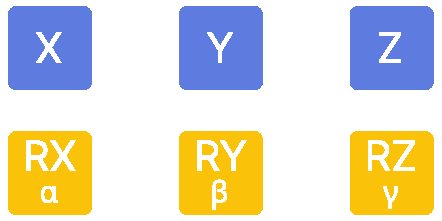
\includegraphics[scale=0.4]{images/1_1_1.pdf}};
        \node at (11.07285, 20.78305) {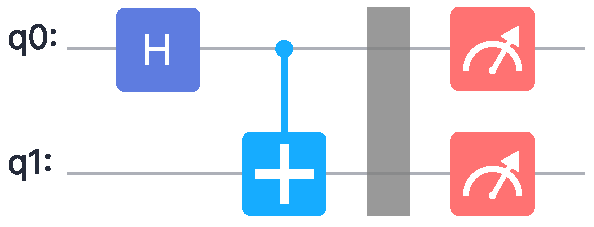
\includegraphics[scale=0.35]{images/1_1_2.pdf}};
        \node at (18.21665, 21.18305){
            \begin{minipage}{0.22\textwidth}
                \ttfamily\scriptsize
                a, b = np.pi, 0.5\\
                ParameterResolver(\{\\
                \hspace*{1em}'a': a, 'b': b\\
                \})
            \end{minipage}
        };

        \node[align=center] at (18.21665, 19.68305) {\textcolor{blue}{$\pi * a+ 1 / 2 * b$}};
        \node at (25.36045, 21.18305-0.2){
            \begin{minipage}{0.22\textwidth}
                \ttfamily\scriptsize
                o = QubitOperator(\\
                \hspace*{1em}'X0 Y1', 'a'\\
                ) + QubitOperator(\\
                \hspace*{1em}'Z2', np.sqrt(2)\\
                )
            \end{minipage}
        };
        \node[align=center] at (25.36045, 19.68305-0.2) {\textcolor{blue}{$aX_0Y_1 + \sqrt{2}Z_2$}};

        % NISQ
        \path[draw=black,line width=0.0794cm] (0.0397, 17.608) rectangle (14.4595, 10.2791);
        \node[align=center, font=\bfseries] at (7.2496, 17.008) {NISQ 算法};

        \path[fill=cffc46d,draw] (0.5159, 16.047) rectangle (6.9453, 14.7505);
        \node[align=center] at (3.7306, 15.39875) {Ansatz 库};

        \path[draw=black] (0.5159, 14.7241) rectangle (6.9453, 10.5436);

        \path[fill=cffc46d,draw] (7.62, 16.0602) rectangle (14.0758, 14.7373);
        \node[align=center] at (10.8479, 15.39875) {VQE};

        \path[fill=cffc46d, draw] (7.62, 13.9435) rectangle (14.0758, 12.6206);
        \node[align=center] at (10.8479, 13.28205) {QAOA};

        \path[fill=cffc46d, draw] (7.62, 11.8269) rectangle (14.0758, 10.504);
        \node[align=center] at (10.8479, 11.16545) {QNN};
        \node at (3.7306, 12.58205) {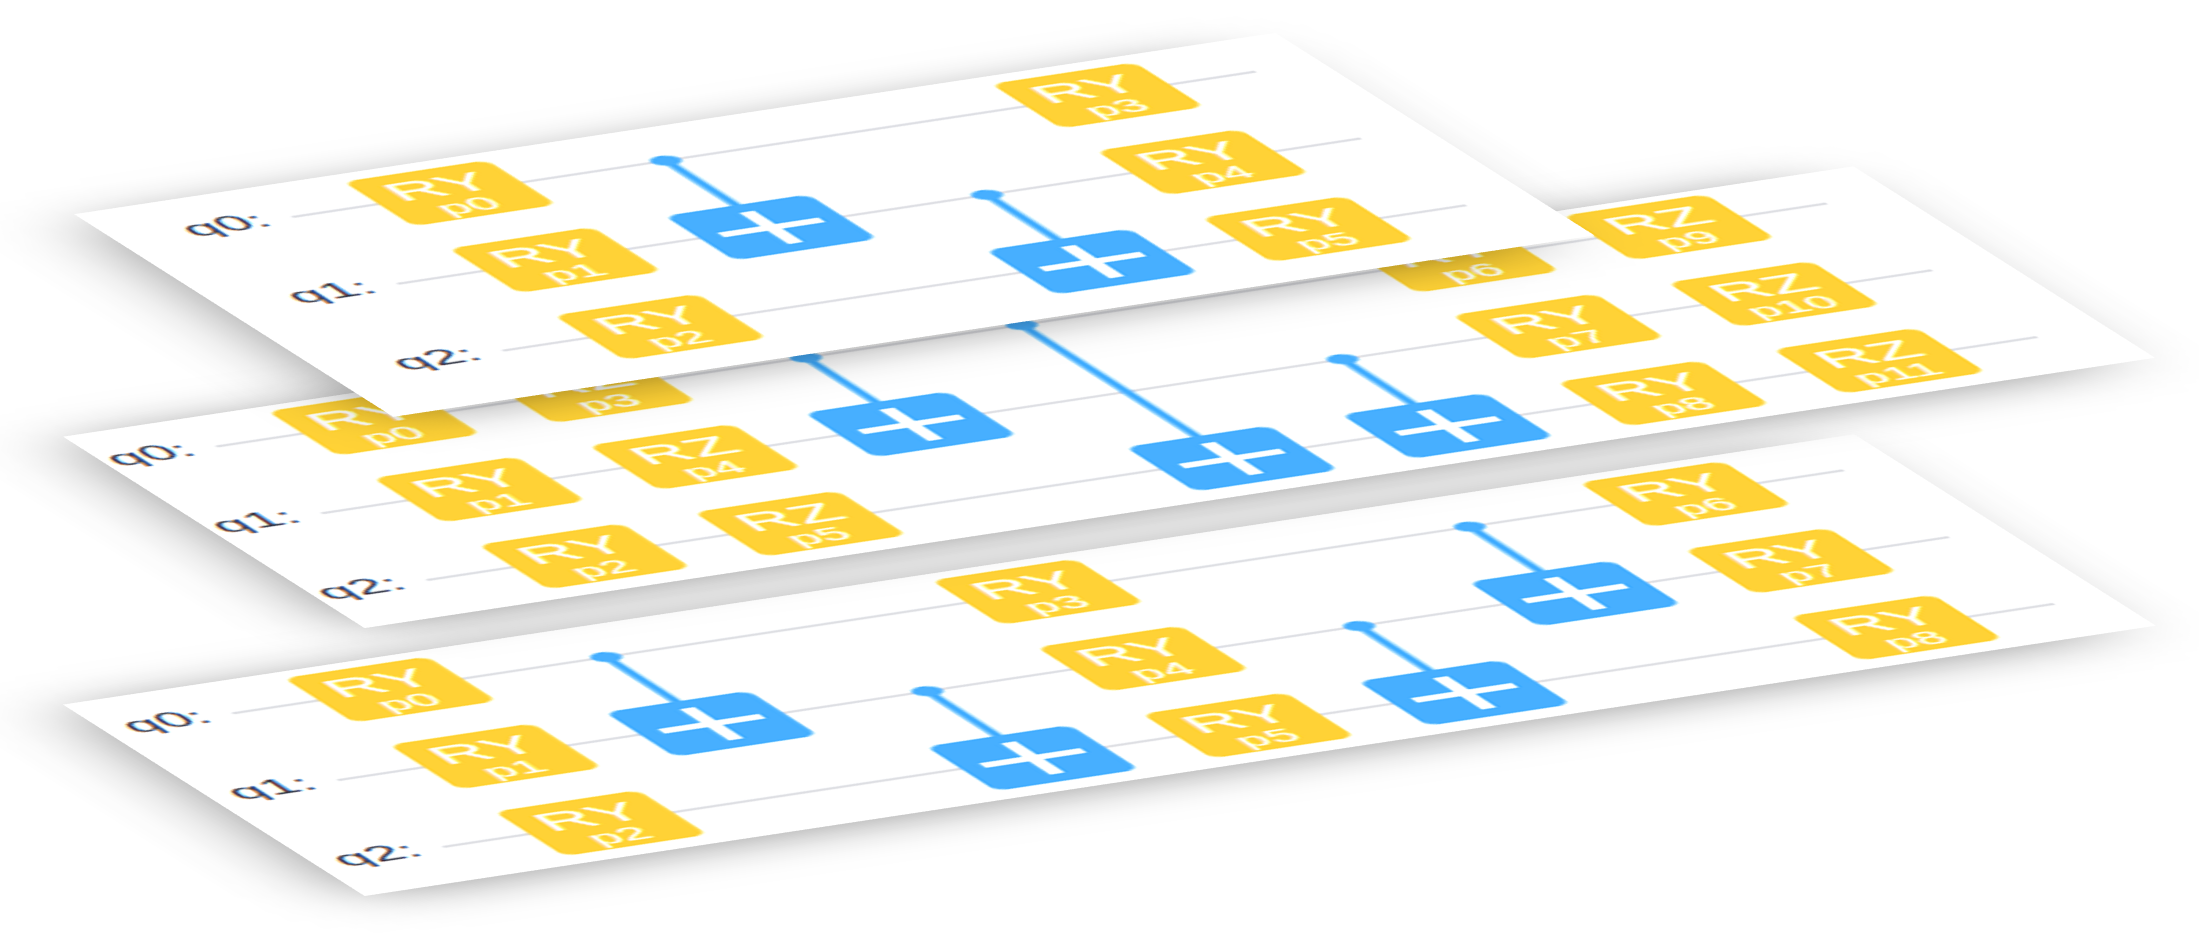
\includegraphics[scale=0.065]{images/1_1_4.jpeg}};


        % Compiler
        \path[draw=black,line width=0.0794cm] (14.8034, 17.608) rectangle (29.2232, 10.2791);
        \node[align=center, font=\bfseries] at (22.0133, 17.008) {编译算法};

        \path[fill=cffc46d,draw] (19.7379, 15.2929) rectangle (28.3633, 13.97);
        \node[align=center] at (24.0506, 14.63145) {基于 DAG 的线路编译器};

        \path[fill=cffc46d,draw] (19.7379, 12.4883) rectangle (28.3633, 11.1654);
        \node[align=center] at (24.0506, 11.82685) {量子比特映射};
        \node at (17.2506, 13.22915) {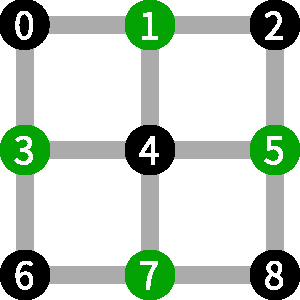
\includegraphics[scale=0.5]{images/1_1_3.pdf}};

        % simulator
        \path[draw=black,line width=0.0794cm] (0.0397, 9.8822) rectangle (14.4595, 3.2941);
        \node[align=center, font=\bfseries] at (7.2496, 9.2822) {量子模拟器};

        \path[fill=c6de1ff] (0.4895, 8.5328) rectangle (14.0626, 7.2364);
        \node[align=center] at (7.2496, 7.8846) {核心模拟算法};

        \path[fill=caffaeb] (0.4763, 6.9585) rectangle (14.0758, 3.5719);
        \node[draw=none] at (5.7, 5.2415) {
            \begin{minipage}{0.4\textwidth}
                \begin{itemize}
                    \item 线路演化
                    \item 采样测量
                    \item 可观测量期望值
                    \item 批模式梯度计算
                \end{itemize}
            \end{minipage}
        };

        % cpu_gpu
        \path[draw=black,line width=0.0794cm] (0.0661, 2.8972) rectangle (14.4859, 0.0397);
        \node[align=center, font=\bfseries] at (7.276,2.2972) {策略细节};

        \path[fill=c0157b4] (0.2646, 1.7992) rectangle (4.6038, 0.2117);
        \node[align=center,text=white] at (2.4342,1.00545) {X86(AVX)};

        \path[fill=c0157b4] (5.0271, 1.7992) rectangle (9.3663, 0.2117);
        \node[align=center,text=white] at (7.1967,1.00545) {GPU(CUDA)};

        \path[fill=c0157b4] (9.7896, 1.7992) rectangle (14.1288, 0.2117);
        \node[align=center,text=white] at (11.9592,1.00545) {Ascend(NENO)};


        % provider
        \path[fill=cf2f2f2] (14.8034, 9.8822) rectangle (29.2232, 3.2941);
        \path[draw=black,line width=0.0794cm,dash pattern=on 0.1588cm off 0.1588cm] (14.8034, 9.8822) rectangle (29.2232, 3.2941);
        \node[align=center, font=\bfseries] at (22.0133, 6.58815) {后端提供者};

        % QPU
        \path[fill=cf2f2f2] (14.8034, 2.8972) rectangle (29.2232, 0.0397);
        \path[draw=black,line width=0.0794cm,dash pattern=on 0.1588cm off 0.1588cm] (14.8034, 2.8972) rectangle (29.2232, 0.0397);
        \node[align=center, font=\bfseries] at (22.0133, 1.46845) {QPU};

    \end{tikzpicture}
    \caption{\MindQuantum\ 的框架}
    \label{fig:framework}
\end{figure*}


\begin{description}
    \item[第一层] 这一层表示框架的基础构件。我们提供多种量子门，以及构造量子线路的便捷方式。为支持变分量子算法，我们还提供参数解析器，用于将部分量子门转换为变分量子门。此外，我们还提供描述各类可观测量的能力。
    \item[第二层] 这一层是算法层，包含通用量子算法和变分量子算法。此外，该层还包括量子编译算法，用于将量子线路编译并映射到量子芯片。
    \item[第三层] 这一层是执行层，会根据执行所使用的硬件划分为量子模拟器和量子芯片后端提供者。在量子模拟器中，我们针对 CPU、GPU 和昇腾架构设计了高性能模拟逻辑，并支持在单精度和双精度模拟模式之间灵活切换。
\end{description}

本白皮书的结构安排如下：第 \hyperref[sec:elements]{\ref*{sec:elements}} 章将介绍 \MindQuantum\ 中用于构造量子线路和可观测量的基本元素；第 \hyperref[sec:backend]{\ref*{sec:backend}} 章将全面展示量子模拟器的使用方法，包括通用状态矢量模拟、密度矩阵模拟、量子化学 CI 子空间模拟和含噪模拟；第 \hyperref[sec:toolbox]{\ref*{sec:toolbox}} 章将讨论 \MindQuantum\ 中与变分量子算法相关的模块，包括各种类型的变分量子线路，以及求解变分量子线路梯度的方法；第 \hyperref[sec:applications]{\ref*{sec:applications}} 章将展示当前学术界近期研究成果中使用 \MindQuantum\ 的示例；第 \hyperref[sec:benchmark]{\ref*{sec:benchmark}} 章将在不同场景中对 \MindQuantum\ 与若干其他量子计算框架进行性能基准比较；第 \hyperref[sec:chip]{\ref*{sec:chip}} 章将说明如何利用 \MindQuantum\ 在真实量子芯片上运行量子算法；第 \hyperref[sec:summary]{\ref*{sec:summary}} 章将对全文进行总结。最后，在第 \hyperref[sec:acknowledgement]{\ref*{sec:acknowledgement}} 章中，我们将感谢所有为 \MindQuantum\ 作出贡献的人，以及在研究中使用 \MindQuantum\ 的用户。


\section{MindSpore Quantum 的基本元素}
\label{sec:elements}

查看本章演示代码：\demonotebook{02}{chapt02} \ \demonotebookgithub{02}{chapt02}

\subsection{数据类型}
% (Zhou Junyuan) The following content is not highly relevant to the main text, so it will not be included in the body.

% In this section, we will introduce the basic data types supported by \MindQuantum. When we run quantum evolution in \MindQuantum, different data types require different sizes of computer memory and lead to different simulation accuracy.
% Before we discuss the supported data types in \MindQuantum, we first briefly review the definition of the floating-point number in modern computers which helps us understand the difference among these data types.
% The first unified technical standard of floating-point arithmetic (IEEE 754) \cite{8766229} was established in 1985 and is widely supported by various hardware today by the Institute of Electrical and Electronics Engineers (IEEE).

% In IEEE 754, a floating-point format is specified by three parts, sign, exponent, and fraction, all of which consist of a ${0,1}$ bit string as shown in Fig.~\ref{fig:ieee}.

% \begin{figure}[h]
%     \centering
%     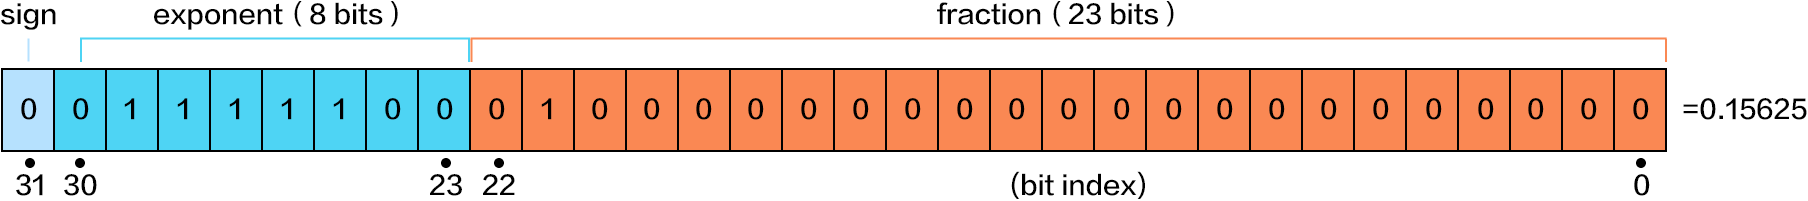
\includegraphics[width=\linewidth]{2.1_figures/Float_example.png}
%     \caption{Floating-point format}
%     \label{fig:ieee}
% \end{figure}

% The sign bit $s$ determines the sign of the number, $s=0$ is positive and $s=1$ is negative.
% The exponent part $e$ is an m-bit unsigned integer, which determines the Maximum and minimum values, and the fraction part $\vec{b}$ with $n$ bits is the true significance that appears in the memory format which determines the precision of the number.

% The real value assumed by a given sign $s$, biased exponent $e$ and fraction $\vec{b}$ as
% \begin{equation}
%     \mathrm{value} = (-1)^{s}\times 2^{e}\times (1+\sum_{i=1}^nb_{23-i}2^{-i}).
% \label[equation]{float-format}
% \end{equation}

% Based on the different numbers of bits, IEEE 754 defined three types of floating-point formats single-, double- and quadruple-precision with 32, 64, and 128 bits, respectively.
% Among them, single- and double-precision are widely used in classical computers.
% In single-precision floating-point format (for short, denoted as Single as follows), there are $1$ bit in the sign part $s$, $8$ bits in the exponent part $e$, and $23$ bits in the fraction part $\vec{b}$.
% In double-precision floating-point format (Double), there are still $1$ bit in the sign part $s$, $11$ bits in the exponent part $e$, and $52$ bits in the fraction part $\vec{b}$.

% The value precision is determined by the number of bits in the fraction part.
% In Single, the fraction part is $\vec{b}=0.b_{22}b_{21}\cdots b{0}$.
% In fact, the first $0$ is default as $1$, so the true fraction part is $1.b_{22}b_{21}\cdots b{0}$, that can explain the Eq.~\eqref{float-format} where $\vec{b}$ plus $1$.
% Then the total precision of Single is 24 bits which approximates $7.22$ decimal digits as $\log_{10}(2^{24}) \approx 7.225$.
% As similar, the total precision of Double is $53$ which can approximate $\log_{10}(2^{53}) \approx 15.95$ decimal digits.
% There is an interesting example showing the difference in the precision of Single and Double,
% \begin{lstlisting}
% z_32=0.1f0+0.2f0
% print(z_32)
% 0.30000001192092896
% z_64=0.1+0.2
% print(z_64)
% 0.30000000000000004
% \end{lstlisting}
% which shows that Single can get $7$ significant digits and Double get $16$ significant digits.


在量子计算中，复数是刻画量子信息的基本工具。复数属于一种在实数基础上引入特定元素 $i$ 后得到的数系，其中 $i$ 称为虚数单位，并满足方程 $i^2=-1$。
复数可以表示为 $c=a+bi$ 的形式，其中 $a$ 和 $b$ 均为实数，$a$ 称为实部，$b$ 称为虚部。

在计算机数字格式中，复数 $c$ 的数据类型由 $a$ 和 $b$ 的类型决定。
通常，如果 $a$ 和 $b$ 均为单精度（Single），则 $c$ 的类型为 complex64（使用 64 位存储 $c$）；如果 $a$ 和 $b$ 均为双精度（Double），则 $c$ 的类型为 complex128（使用 128 位存储 $c$）。

在不同编程语言中，虚数单位的符号可能有所不同。
例如，在 C 语言中，$i$ 表示为 $I$；在 Python 中，则表示为 $1j$。
\MindQuantum\ 支持单精度和双精度浮点格式，同时也支持它们对应的复数格式；这些复数格式对于模拟量子演化不可或缺。
这些数据类型可以与 NumPy \cite{harris2020array} 包中的对应数据类型便捷转换。它们具有相同的数学性质，但在 \MindQuantum\ 中使用时，相比直接声明为 NumPy 数据类型更便于框架内部处理。

\begin{lstlisting}
import numpy as np
import mindquantum as mq

# 支持不同类型
all_types = [mq.float32, mq.float64, mq.complex64, mq.complex128]

# 与 numpy 类型相互转换
mq_float64 = mq.to_mq_type(np.float64)
numpy_float64 = mq.to_np_type(mq.float64)
\end{lstlisting}

指数墙是在经典计算机上模拟量子系统面临的主要障碍。
随着量子系统规模增大，所需经典资源会呈指数增长。
一个包含 $N$ 个量子比特的量子态可以由 $2^N$ 个振幅描述，而所有振幅都是复数。

如果要存储一个 $N=20$ 的量子态，其中包含 $2^{20}$ 个振幅，且所有振幅均以单精度（Complex64）表示，则所需经典内存为
\begin{equation}
    G=2^{20}\times 64 \mathrm{bits} = 8 \mathrm{MB}.
\end{equation}

如果使用双精度复数表示振幅，则内存需求为 $G=2^{20}\times 128 \mathrm{bits}=16 \mathrm{MB}$。下面的表格展示了在不同数据精度下存储全振幅量子态所需的内存消耗。

\begin{table}[ht]
    \begin{tabular}{ccc}
        \toprule
        量子比特数 & Complex128 & Complex64 \\
        \midrule
        6            & 1kB        & 0.5kB     \\
        16           & 1MB        & 0.5MB     \\
        26           & 1GB        & 0.5GB     \\
        30           & 16GB       & 8GB       \\
        36           & 1TB        & 0.5TB     \\
        40           & 16TB       & 8TB       \\
        \bottomrule
    \end{tabular}
    \caption{存储全振幅量子态的内存消耗。}
    \label{tab:mem_consume}
\end{table}

不难看出，双精度所需存储空间是单精度的两倍，因为每个双精度振幅占用 $128$ 位，而每个单精度振幅占用 $64$ 位。
虽然双精度需要更多空间，通常也需要更多计算时间（这取决于具体处理单元），但它能够提供更高精度；这对于量子计算中的一些任务非常重要，例如求解量子哈密顿量的本征值。
事实上，在相同内存资源下，使用单精度表示振幅相比双精度最多只能多模拟一个量子比特。
因此，如果内存资源充足，我们强烈建议优先使用双精度复数。


\subsection{参数解析器}
\subsubsection{MindQuantum 中的参数}
参数化量子门或量子线路是量子计算的重要组成部分，尤其对于量子-经典混合算法而言更是如此。
在 \MindQuantum\ 中，我们提供了 Python 类 \code{mindquantum.core.ParameterResolver}，用于高效管理这些经典参数。
假设我们希望初始化一个参数化量子门，而该参数的值可能会在优化过程中发生变化。
\ParameterResolver\ 通过将每个参数表示为唯一符号来解决这一问题，例如 $\theta=0.1$，其中 $\theta$ 是参数符号，$0.1$ 是对应数值。
这样，在 \MindQuantum\ 中编写代码时，我们就可以使用符号而非实际数值来表示参数。
声明 \ParameterResolver\ 实例时，只需以 Python dict 的形式给出符号与数值，其中符号作为 dict 的键，数值作为 dict 的值：

\begin{lstlisting}
import numpy as np
from mindquantum.core.parameterresolver import ParameterResolver

# 使用 dict 构造 ParameterResolver
pr1 = ParameterResolver({'theta': np.pi})

# 使用符号 'a' 构造 ParameterResolver
pr2 = ParameterResolver('a')

# 这等价于
pr3 = ParameterResolver({'a': 1.0})

# 声明一个常数
pr4 = ParameterResolver(3)

# 也支持算术运算符
pr5 = pr1 + pr2 * np.sqrt(2)
print(pr5.expression())
\end{lstlisting}

\code{pr5} 的表达式将显示为 $\sqrt{2}*a + \pi*\text{theta}$。

当 \MindQuantum\ 模拟参数化线路时，\ParameterResolver\ 会将线路中的符号替换为 \ParameterResolver\ 中声明的对应实际数值。

在量子-经典混合算法中，参数通常由 SGD、ADAM 和 BFGS 等梯度下降方法进行优化。声明 \ParameterResolver\ 实例时，默认情况下所有参数都需要参与求导。
不过，我们也可以按照如下方式显式声明某个参数是否需要求导：

\begin{lstlisting}
params.no_grad_part('theta')
\end{lstlisting}

这里，\code{params} 是一个 \ParameterResolver\ 实例。调用 \code{no_grad_part('theta')} 方法用于指定名为 \code{theta} 的参数不可求导。这意味着在后续任何优化步骤或梯度计算中，\code{theta} 参数都将被排除在外。

在混合算法中，参数化量子门或量子线路通常分为两部分：编码器（encoder）和 ansatz。编码器将经典数据编码到量子态中；ansatz 则是对未知函数形式所作的假设，我们可以通过优化 ansatz 来近似问题的解。默认情况下，\ParameterResolver\ 中的所有参数都会初始化为 ansatz 参数。我们可以通过以下方式在编码器参数和 ansatz 参数之间转换：

\begin{lstlisting}
# 将所有参数声明为编码器参数
params.as_encoder()

# 将所有参数声明为 ansatz 参数
params.as_ansatz()

# 将给定符号声明为编码器参数
params.encoder_part('theta')

# 将给定符号声明为 ansatz 参数
params.ansatz_part('theta')
\end{lstlisting}

更具体的示例请参见第 \ref{sec:rotate_three_states} 节。

也可以按照如下方式修改 \ParameterResolver\ 实例中参数的数据类型：
\begin{lstlisting}
# 将 params 的数据类型重置为 mq.complex128
params.astype(mq.complex128)
\end{lstlisting}

\subsubsection{参数生成器}

此外，\MindQuantum\ 还提供了一个用于快速生成参数的强大工具：\PRGenerator。
\begin{lstlisting}
from mindquantum.core.parameterresolver import PRGenerator

prg = PRGenerator(suffix='a')
a = prg.new()
b = prg.new()
print(a)
print(b)
print(len(prg.all_pr))
\end{lstlisting}
输出为：
\begin{lstlisting}
p0_a
p1_a
2
\end{lstlisting}


\subsection{量子门}
本节介绍量子门，并展示其在 \MindQuantum\ 中的使用方式。我们将量子门分为三类：固定量子门、参数化量子门和自定义量子门。此外，我们使用 \code{on()} 方法设置目标量子比特和控制量子比特，并使用 \code{controlled()} 函数为多个量子门添加控制量子比特。

\subsubsection{量子门概述}

在量子计算中，量子门是操控量子比特的基本操作，而量子比特是量子信息的基本单位。类似于作用在比特上的经典逻辑门，量子门作用在量子比特上，并在数学上由酉矩阵表示，从而保持量子态的归一性和可逆性。

量子门通过执行旋转、翻转和生成纠缠等操作，成为构造量子线路和实现量子算法的核心。这些操作赋予量子计算机区别于经典计算机的独特计算能力。

量子门可以根据其作用的量子比特数量进行分类：单量子比特门修改单个量子比特的状态，多量子比特门则促成量子比特之间的相互作用，从而实现复杂量子操作和纠缠。量子门也可以分为非参数化门（例如 \X、\Y、\Z、\H）和参数化门（例如 \RX、\RY、\RZ），后者提供了额外的计算灵活性。在 \MindQuantum\ 中，这些量子门都可以便捷构造，其中也包括使用 \ParameterResolver\ 的参数化量子门。

\subsubsection{固定量子门}
固定量子门对量子态执行特定操作，并由酉矩阵表示。以下给出量子比特态 $\ket{\phi}=a\ket{0}+b\ket{1}$ 上的一些示例：

\begin{align*}
    I\ket{\phi} & =
    \begin{bmatrix}
        1 &  & 0 \\
        0 &  & 1
    \end{bmatrix}
    \begin{bmatrix}
        a \\
        b
    \end{bmatrix}=
    \begin{bmatrix}
        a \\
        b
    \end{bmatrix},  \\
    X\ket{\phi} & =
    \begin{bmatrix}
        0 &  & 1 \\
        1 &  & 0
    \end{bmatrix}
    \begin{bmatrix}
        a \\
        b
    \end{bmatrix}=
    \begin{bmatrix}
        b \\
        a
    \end{bmatrix},  \\
    Y\ket{\phi} & =
    \begin{bmatrix}
        0 & -i \\
        i & 0
    \end{bmatrix}
    \begin{bmatrix}
        a \\
        b
    \end{bmatrix}=
    \begin{bmatrix}
        -bi \\
        ai
    \end{bmatrix},  \\
    Z\ket{\phi} & =
    \begin{bmatrix}
        1 & 0 \\
        0 & -1
    \end{bmatrix}
    \begin{bmatrix}
        a \\
        b
    \end{bmatrix}=
    \begin{bmatrix}
        a \\
        -b
    \end{bmatrix}, \\
    H\ket{\phi} & =
    \frac{1}{\sqrt{2}}
    \begin{bmatrix}
        1 & 1  \\
        1 & -1
    \end{bmatrix}
    \begin{bmatrix}
        a \\
        b
    \end{bmatrix}=
    \frac{1}{\sqrt{2}}
    \begin{bmatrix}
        a+b \\
        a-b
    \end{bmatrix}.
\end{align*}

\MindQuantum\ 中的示例用法如下：
\begin{lstlisting}
from mindquantum.core.gates import H, SWAP

h = H.on(0)
swap = SWAP.on([0, 1])
print(swap)
\end{lstlisting}
输出为：
\begin{lstlisting}
SWAP(0 1)
\end{lstlisting}

\subsubsection{参数化量子门}
Pauli 矩阵是一类非常重要的矩阵，它们构成了算符空间的一组基。当 Pauli 矩阵出现在指数中时，可以得到三类有用的酉算符，即分别对应 $\hat{x}, \hat{y}, \hat{z}$ 方向的旋转算符，定义如下：

\begin{align*}
    Rx(\theta) & =
    e^{-\frac{i\theta X}{2}}=
    \cos{\frac{\theta}{2}}I-i\sin{\frac{\theta}{2}}X \\
               & =\begin{bmatrix}
        \cos{\frac{\theta}{2}}   &  & -i\sin{\frac{\theta}{2}} \\
        -i\sin{\frac{\theta}{2}} &  & \cos{\frac{\theta}{2}}
    \end{bmatrix},        \\
    Ry(\theta) & =
    e^{-\frac{i\theta Y}{2}}=
    \cos{\frac{\theta}{2}}I-i\sin{\frac{\theta}{2}}Y \\
               & =    \begin{bmatrix}
        \cos{\frac{\theta}{2}} &  & -\sin{\frac{\theta}{2}} \\
        \sin{\frac{\theta}{2}} &  & \cos{\frac{\theta}{2}}
    \end{bmatrix},    \\
    Rz(\theta) & =
    e^{-\frac{i\theta Z}{2}}=
    \cos{\frac{\theta}{2}}I-i\sin{\frac{\theta}{2}}Z \\
               & =    \begin{bmatrix}
        e^{\frac{-i\theta}{2}} &  & 0                     \\
        0                      &  & e^{\frac{i\theta}{2}}
    \end{bmatrix}.
\end{align*}


由于 $2\times2$ 矩阵的数量是无限的，量子门的数量也同样是无限的。根据 Z-Y 分解，任意单量子比特酉矩阵 $U$ 都可以表示为 $U=e^{i\alpha}Rz(\beta)Ry(\gamma)Rz(\delta)$。因此，为了构造通用量子门，需要使用参数来构造旋转门。由于 \ParameterResolver\ 支持三种初始化方式，\MindQuantum\ 也提供了三种初始化方法。以 RX 门为例：

\begin{lstlisting}
from mindquantum.core.gates import RX
from mindquantum.core.parameterresolver import ParameterResolver as PR
import numpy as np

rx1 = RX(0.5)
rx2 = RX('a')
rx3 = RX({'a': 0.2, 'b': 0.5})

a, b = PR('a'), PR('b')
rx4 = RX(0.2 * a + 0.5 * b)

mat_rx1 = rx1.matrix()
mat_rx4 = rx4.matrix(pr={'a': 1, 'b': 2})
\end{lstlisting}

请注意，在上述示例中，\code{rx1} 实际上是一个非参数化量子门，因为我们已经设置了旋转角 $\theta = 0.5$。

\subsubsection{自定义量子门}
在某些具体应用中，有时需要创建任意量子门。在 \MindQuantum\ 中，可以通过两种方法构造自定义量子门：

\textit{通用矩阵门} -- 如果已知某个量子门的矩阵表示，就可以在 \MindQuantum\ 中方便地构造该门。初始化 \UnivMathGate\ 需要两个参数，即量子门名称和矩阵值。如果矩阵不是酉矩阵，状态矢量将无法保持归一化。
示例：
\begin{lstlisting}
from mindquantum.core.gates import UnivMathGate
import numpy as np

x_mat = np.array([[0,1],[1,0]])
custom_X_gate = UnivMathGate('custom_X', x_mat).on(0, 1)
print(custom_X_gate)
\end{lstlisting}

输出：
\begin{lstlisting}
custom_X(0 <-: 1)
\end{lstlisting}

\textit{通用参数化门} -- 在某些应用中，我们需要构造参数会发生变化的参数化量子门。在 \MindQuantum\ 中，可以通过 \geneunivparameterizedgate\ 方便地构造自定义参数化量子门，其用法与 \RX\ 门基本一致。初始化这类量子门需要两个参数：其一是一个仅使用一个参数（类似 \RX\ 中的 theta）来生成酉矩阵的函数或方法，需要注意的是，即使生成的矩阵不是酉矩阵，也不会报错；其二是生成该矩阵导数的函数或方法，用于计算梯度。该方法支持生成任意量子比特算符，并可以通过 numba.JIT 加速性能。

示例：
\begin{lstlisting}
from mindquantum.core.gates import gene_univ_parameterized_gate

def matrix(theta):
    return np.array([[np.exp(1j * theta), 0],
                     [0, np.exp(-1j * theta)]])

def diff_matrix(theta):
    return 1j * np.array([[np.exp(1j * theta), 0],
                          [0, -np.exp(-1j * theta)]])

TestGate = gene_univ_parameterized_gate('Test', matrix, diff_matrix)

# 非参数化用法
test1 = TestGate(0.5).on(0)

# 参数化用法
test2 = TestGate('a').on(0)
\end{lstlisting}

\subsubsection{\texttt{on()} 方法}
对于某些受控量子门，我们需要指定量子门的目标量子比特和控制量子比特。在 \MindQuantum\ 中，可以通过 \code{on()} 方法实现该功能。此方法接收两个参数：一个是目标量子比特，另一个是控制量子比特；二者都可以是单个量子比特或多个量子比特。值得强调的是，任意量子门都可以添加任意控制操作。

示例：
\begin{lstlisting}
from mindquantum.core.gates import X

x = X.on(0, [1, 2])
print('Target qubit:{}, Control qubits:{}'.format(x.obj_qubits, x.ctrl_qubits))
\end{lstlisting}

输出：
\begin{lstlisting}
Target qubit:[0], Control qubits:[1, 2]
\end{lstlisting}

\subsubsection{\texttt{controlled()} 函数}
除 \code{on()} 方法外，我们还可以通过 \code{controlled()} 函数添加控制量子比特。\code{controlled()} 函数用于为任意量子线路或量子算符添加控制量子比特（可以有多个）。例如，我们构造一个仅包含两个量子比特的量子线路，并通过 \code{controlled()} 方法为其添加一个控制量子比特 q2：
\begin{lstlisting}
from mindquantum.algorithm.library import qft
from mindquantum.core.circuit import controlled

u1 = qft(range(2))
u2 = controlled(u1)
u2 = u2(2)
u2.svg()
\end{lstlisting}

如图~\ref{fig:controlled-method} 所示，此时 QFT 线路由 q2 控制。

\begin{figure}[h]
    \centering
    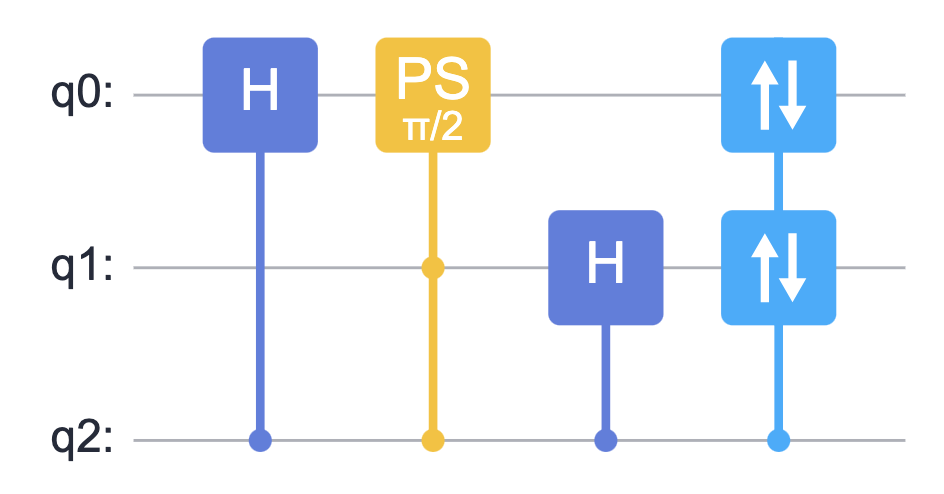
\includegraphics[width=0.9\linewidth]{2.3_figures/control.png}
    \caption{添加控制量子比特}
    \label{fig:controlled-method}
\end{figure}

此外，我们还可以批量为量子线路添加控制量子比特。在下面的示例中，目标量子比特分别为 q0 和 q1，对应的控制量子比特分别为 q2 和 q3：
\begin{lstlisting}
u = controlled(qft)
u = u([2, 3], [0, 1])
u.svg()
\end{lstlisting}

结果如图~\ref{fig:batch-control} 所示。
\begin{figure}[h]
    \centering
    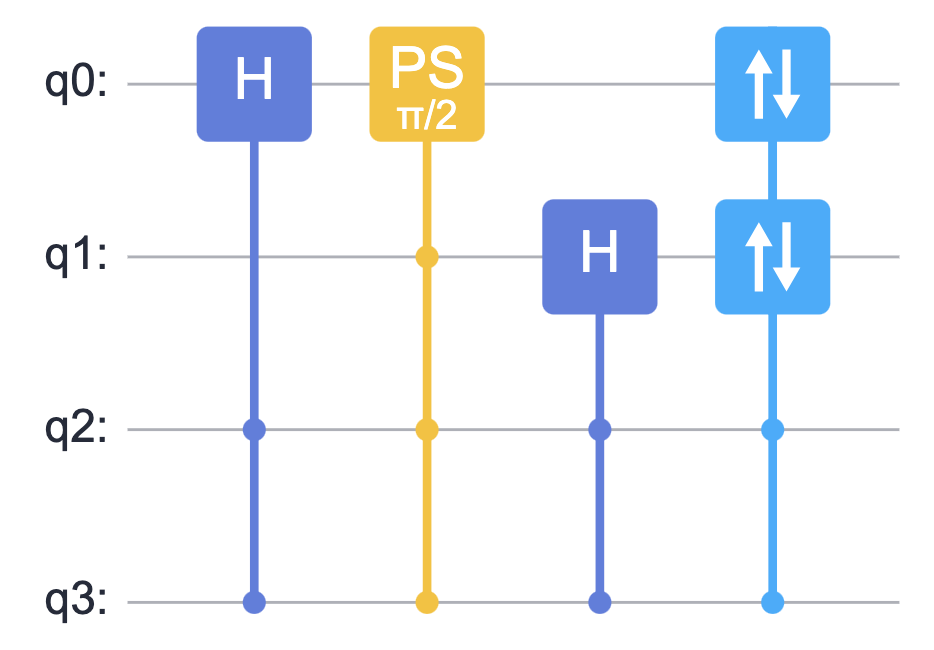
\includegraphics[width=0.9\linewidth]{2.3_figures/batch_control.png}
    \caption{批量添加控制量子比特}
    \label{fig:batch-control}
\end{figure}


\subsection{量子线路}
量子线路是量子计算或量子算法中施加在量子比特上的量子门序列的图形化表示。类似于由逻辑门组成并操控经典比特的经典数字电路，量子线路由操控量子比特的量子门组成。

\subsubsection{构造量子线路}
在 \MindQuantum\ 中，我们使用 \Circuit\ 表示量子线路：

\begin{lstlisting}
from mindquantum.core.circuit import Circuit
circ = Circuit()
\end{lstlisting}

向 \Circuit\ 中添加量子门有几种基本操作：
\begin{itemize}
    \item list：使用量子门列表直接构造量子线路。
    \item \code{+=}：使用 \code{+=} 将量子门添加到线路中。
    \item \code{Circuit.x}：向线路中添加 X 门。
\end{itemize}
\begin{lstlisting}
from mindquantum.core.gates import H, Y, X, Z
circ = Circuit([X.on(0), Y.on(1)])
circ += H.on(0)
circ += Y.on(1, 0)
circ.x(1, 0)
circ.z(2, [0, 1])
\end{lstlisting}

结果如图~\ref{fig:Quantum-Circuit} 所示。

\subsubsection{展示量子线路}
SVG（Scalable Vector Graphics，可缩放矢量图形）基于 XML 标记语言，用于描述二维矢量图形。\MindQuantum\ 提供了将量子线路导出为 SVG 格式的函数。
\begin{lstlisting}
circ.svg().to_file(filename='circuit.svg')
\end{lstlisting}
\begin{figure}[h]
    \begin{center}
        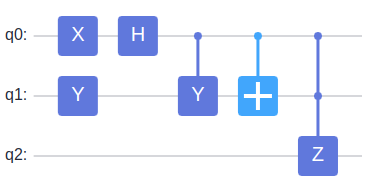
\includegraphics[width=0.9\linewidth]{images/2_4_circuit.png}
    \end{center}
    \caption{量子线路。}
    \label{fig:Quantum-Circuit}
\end{figure}
请注意，如果处于 Jupyter Notebook 环境中，可以直接通过 \code{circ.svg()} 获取 SVG 图像。


\subsubsection{常用接口}

量子线路是量子算法的基本元素，\MindQuantum\ 为 \Circuit\ 提供了许多实用方法。

\begin{itemize}
    \item \propnqubits：获取量子线路的量子比特数量。
    \item \propparamsname：获取线路中的参数名称。
    \item \prophasmeasuregate：获取线路是否包含测量门。
    \item \methodmatrix：获取线路矩阵。
    \item \methodgetqs：获取最终量子态。
    \item \methodsummary：获取当前线路的信息，包括模块数量、量子门数量、非参数化量子门数量、参数化量子门数量以及参数数量。
\end{itemize}

\subsubsection{量子线路上的高级操作}

构造大规模量子线路并不总是直接明了。为此，\MindQuantum\ 提供了一些预定义方法，使 \Circuit\ 更加易用。例如，设原始量子线路为：

\begin{lstlisting}
from mindquantum.core.circuit import *

circ = Circuit().h(0).rx('a', 2, 0)
\end{lstlisting}

\begin{figure}[H]
    \begin{center}
        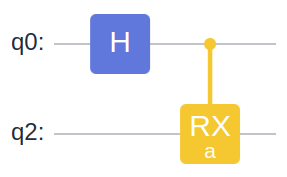
\includegraphics[width=0.4\linewidth]{images/2_4_ori_circ.png}
    \end{center}
    \caption{待操作的量子线路。}
\end{figure}
下面展示如何对该量子线路进行操作：


\begin{enumerate}
    \item \methodcompress{circ}：将所有量子比特压缩到前 $n$ 个量子比特上。\par
          \begin{minipage}{\linewidth}
              \centering
              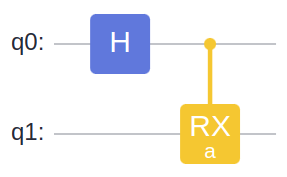
\includegraphics[width=0.4\linewidth]{images/2_4_compress_circ.png}
          \end{minipage}
    \item \methodcontrol{circ}{1}：为该线路添加控制量子比特。\par
          \begin{minipage}{\linewidth}
              \centering
              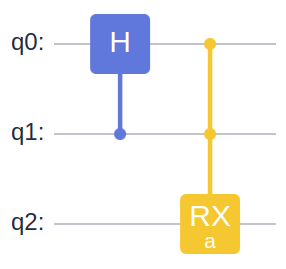
\includegraphics[width=0.4\linewidth]{images/2_4_ctrl_circ.png}
          \end{minipage}
    \item \methoddagger{circ}：获取厄米共轭版本。\par
          \begin{minipage}{\linewidth}
              \centering
              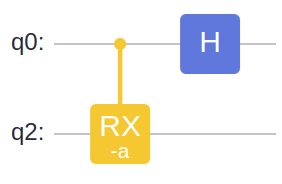
\includegraphics[width=0.4\linewidth]{images/2_4_dagger_circ.png}
          \end{minipage}
    \item \methodapply{circ}{[2, 1]}：将线路应用到其他量子比特上。\par
          \begin{minipage}{\linewidth}
              \centering
              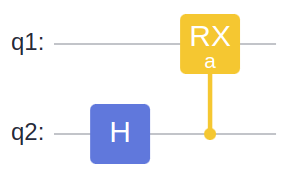
\includegraphics[width=0.4\linewidth]{images/2_4_apply_circ.png}
          \end{minipage}
    \item \methodreverse{circ}：反转线路中的量子比特顺序。\par
          \begin{minipage}{\linewidth}
              \centering
              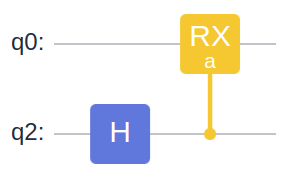
\includegraphics[width=0.4\linewidth]{images/2_4_reverse_circ.png}
          \end{minipage}
    \item \methodshift{circ}{2}：按给定步长平移量子比特范围。\par
          \begin{minipage}{\linewidth}
              \centering
              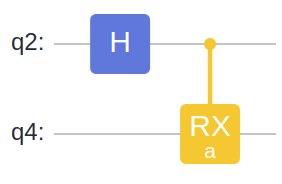
\includegraphics[width=0.4\linewidth]{images/2_4_shift_circ.png}
          \end{minipage}
\end{enumerate}


\subsection{可观测量与哈密顿量}
Richard Feynman 曾提出，多体物理系统模拟是量子计算的主要应用之一。在众多多体物理模型中，我们重点关注 Heisenberg 模型和 Fermi-Hubbard 模型。这些模型的哈密顿量可以表示如下：

\begin{align*}
    H_\text{Heisenberg}    & = -J\sum_{<i,j>}\sigma_i\otimes \sigma_j-h\sum_i\sigma_i,                                            \\
    H_\text{Fermi-Hubbard} & = -\sum_{<i,j>,\sigma}\left(a_{i\sigma}^\dagger a_{j\sigma} + a_{j\sigma}^\dagger a_{i\sigma}\right) \\
                           & + U\sum_i n_{i\uparrow}n_{i\downarrow}.
\end{align*}

在 \MindQuantum\ 中，借助 \QubitOperator\ 和 \FermionOperator\ 可以方便地构造这些哈密顿量。

\subsubsection{量子比特算符}

在 Heisenberg 模型中，$\sigma_i$ 表示 Pauli 算符。Pauli 算符的矩阵形式为：

\begin{align*}
    \sigma_X & = \begin{pmatrix}
        0 & 1 \\
        1 & 0
    \end{pmatrix}, \sigma_Y = \begin{pmatrix}
        0 & -i \\
        i & 0
    \end{pmatrix}, \\
    \sigma_I & =\begin{pmatrix}
        1 & 0 \\
        0 & 1
    \end{pmatrix}, \sigma_Z = \begin{pmatrix}
        1 & 0  \\
        0 & -1
    \end{pmatrix}.
\end{align*}
在 \MindQuantum\ 中，\QubitOperator\ 用于构造这类算符。给定 Pauli 字符串 $\sigma_{X,3}\otimes \sigma_{Y,1}\otimes \sigma_{Z,0}=X_3 Y_1 Z_0$，即在第 3、1、0 号量子比特上分别作用 Pauli $X$、Pauli $Y$ 和 Pauli $Z$，可以通过如下方式方便地构造：

\begin{lstlisting}
from mindquantum.core.operators import QubitOperator

ops = QubitOperator('Z0 Y1 X3')
\end{lstlisting}
请注意，由于 $[Z_0, Y_1]= [Z_0,X_3] = [Y_1, X_3]=0$，Pauli 字符串中各 Pauli 项的顺序并不影响结果。

\QubitOperator\ 也支持算术运算，以便构造更复杂的算符：

\begin{lstlisting}
from mindquantum.core.operators import QubitOperator
from mindquantum.core.parameterresolver import ParameterResolver as PR

op1 = QubitOperator('X0')
op2 = QubitOperator('Z1', 'a')
op3 = QubitOperator('Y1')
op4 = 2 * op1 * op2 + op3 * PR('b')
print(op4)
print(op4.subs({'a':1, 'b':2}).matrix().toarray())
\end{lstlisting}
输出为：
\begin{lstlisting}
2*a [X0 Z1] +
  b [Y1]

[[ 0.+0.j  2.+0.j  0.-2.j  0.+0.j]
 [ 2.+0.j  0.+0.j  0.+0.j  0.-2.j]
 [ 0.+2.j  0.+0.j  0.+0.j -2.+0.j]
 [ 0.+0.j  0.+2.j -2.+0.j  0.+0.j]]
\end{lstlisting}
在最后一行中，我们使用 \code{.subs} 设置参数值，并使用 \code{.matrix} 得到 CSR 格式的稀疏矩阵。

\subsubsection{费米子算符}

在 Fermi-Hubbard 模型中，$a_i^\dagger$ 和 $a_i$ 是费米子粒子的产生算符和湮灭算符。不同于 Pauli 算符，费米子算符满足反对易关系：
\begin{align*}
    \{a_i, a_j^\dagger\} & = a_ia_j^\dagger + a_j^\dagger a_i = \delta_{ij}, \\
    \{a_i, a_j\}         & = \{a_i^\dagger, a_j^\dagger\}=0.
\end{align*}
在量子比特系统中，作用在态 $\ket{0}$ 和 $\ket{1}$ 上的产生算符与湮灭算符满足如下规则：
\begin{align*}
    a\ket{0}          & =0,        & a\ket{1}          & =\ket{0}, \\
    a^\dagger \ket{0} & = \ket{1}, & a^\dagger \ket{1} & =0.
\end{align*}

产生算符与湮灭算符的矩阵形式为：

\begin{align*}
    a=\begin{pmatrix}
        0 & 1 \\
        0 & 0
    \end{pmatrix},
    a^\dagger=\begin{pmatrix}
        0 & 0 \\
        1 & 0
    \end{pmatrix}.
\end{align*}
在 \MindQuantum\ 中，可以使用 \FermionOperator\ 构造费米子算符。假设我们先在第 1 号量子比特上产生一个态，再在第 0 号量子比特上湮灭一个态，即 $a_1^\dagger\otimes a_0$，则可以通过如下方式构造：
\begin{lstlisting}
from mindquantum.core.operators import FermionOperator
op1 = FermionOperator('1^ 0')
\end{lstlisting}
在费米子字符串中，我们使用 \verb|^| 表示 $\dagger$，并使用数字标记对应量子比特。\FermionOperator\ 的算术运算与 \QubitOperator\ 非常相似。


\subsubsection{算符函数}

\MindQuantum\ 还为算符提供了许多高级函数。以下是一些示例：

- \methodcommutator{op1}{op2}：输出两个算符的对易子。

\begin{lstlisting}
from mindquantum.core.operators import QubitOperator, FermionOperator, commutator
qub_op1 = QubitOperator("X1 Y2")
qub_op2 = QubitOperator("X1 Z2")
commutator(qub_op1, qub_op1)  # 0
commutator(qub_op1, qub_op2)  # (2j) [X2]
\end{lstlisting}

- \methodcountqubits{op1}：在删除未使用量子比特前统计量子比特数量。

\begin{lstlisting}
from mindquantum.core.operators import QubitOperator,FermionOperator, count_qubits
qubit_op = QubitOperator("X1 Y2")
count_qubits(qubit_op)  # 3
fer_op = FermionOperator("1^")
count_qubits(fer_op)  # 2
\end{lstlisting}


- \methodhermitianconj{op1}：获取给定算符的厄米共轭。

\begin{lstlisting}
from mindquantum.core.operators import FermionOperator, hermitian_conjugated
fer_op = FermionOperator("1^ 3")
hermitian_conjugated(fer_op)
\end{lstlisting}

\subsubsection{变换}
费米子系统的量子模拟具有挑战性。为了有效降低在量子硬件上模拟费米子哈密顿量所需的资源，可以使用量子比特模拟费米子，这涉及费米子哈密顿量与量子比特哈密顿量之间的转换。\MindQuantum\ 提供了 \code{mindquantum.algorithm.nisq.Transform} 模块，用于在费米子算符（\FermionOperator）和量子比特算符（\QubitOperator）之间进行变换。该模块提供如下函数：
\begin{itemize}
    \item \methodjordanwigner：应用 Jordan-Wigner 变换，该变换通过如下方式将费米子湮灭算符（费米子）映射到量子比特算符：
          \begin{equation}
              \begin{split}
                  a_j^{\dagger} \to {\sigma}_j^{-} X \prod_{i=0}^{j-1} {\sigma}^Z_i \\
                  a_j \to {\sigma}_j^{+} X \prod_{i=0}^{j-1} {\sigma}^Z_i,
              \end{split}
          \end{equation}
          其中 ${\sigma}_j^{+} = {\sigma}_j^X+i{\sigma}_j^Y$、${\sigma}_j^{-} = {\sigma}_j^X-i{\sigma}_j^Y$ 分别为升自旋算符和降自旋算符。算符 $\prod_{i=0}^{p-1} {{\sigma}^Z_i}$ 称为“奇偶算符”，其本征值为 $\pm 1$，因为它用于测量从索引 0 到 $p-1$ 的量子比特中处于向下态（或“$-1$”态）的数量是偶数还是奇数。如果该数量为偶数，算符给出 $+1$；如果为奇数，则给出 $-1$。该变换保持了初始占据数的局域性。该方法的问题在于，由于奇偶算符具有非局域性，模拟单个费米子算符所需的额外量子比特操作数量会按 $O(n)$ 缩放。
    \item \methodparity：应用奇偶变换，该变换使用量子比特 $j$ 存储截至轨道 $j$ 的所有占据轨道的奇偶性。也就是说，可以令量子比特 $j$ 存储 $p_j = (\sum_{i=0}^j f_i) mod 2$。其中，$f_i$ 表示第 $i$ 个轨道的占据数，可以为 0（未占据）或 1（已占据）。这种在量子比特态中编码费米子态的方式称为 $parity$ 基。占据数基态可以表示为向量（例如 $(j_7,...,j_1,j_0)^T$），并可以按如下方式映射到奇偶基：
          \begin{equation}
              p_i = \sum_j {[\pi_n]_{ij} f_j},
          \end{equation}
          其中 $n$ 是轨道数量，$\pi_n$ 是如下定义的 ($n \times n$) 矩阵：
          \begin{equation}
              [\pi_n]_{ij} =
              \begin{cases}
                  1 & i<j     \\
                  0 & i\geq j \\
              \end{cases}.
          \end{equation}
          因而，产生算符和湮灭算符在奇偶基中的表示为：
          \begin{equation}
              \begin{split}
                  a_j^{\dagger} \to \frac{1}{2} (\prod_{i=j+1}^n ({\sigma}^X_i X))({\sigma}^X_j - i{\sigma}^Y_j) X {\sigma}^Z_{j-1} \\
                  a_j \to \frac{1}{2} (\prod_{i=j+1}^n ({\sigma}^X_i X))({\sigma}^X_j + i{\sigma}^Y_j) X {\sigma}^Z_{j-1}.
              \end{split}
          \end{equation}
    \item \methodbravyikitaev \cite{bravyi2002fermionic, fenwick1994new}：前两种方法在用量子比特编码表示费米子算符所需信息的意义上是对偶的。对于占据数基及其对应的 Jordan-Wigner 变换，占据信息是局域存储的，但奇偶信息是非局域的；而在奇偶基方法及其相应算符变换中，奇偶信息是局域存储的，但占据信息是非局域的。
          Bravyi-Kitaev 变换是一种折中方案，它平衡了占据信息和奇偶信息的局域性，从而提高模拟效率。在该方案中，量子比特存储一组 $2^x$ 个轨道的奇偶性，其中 $x \geq 0$。索引为 $j$ 的量子比特始终存储轨道 $j$。当 $j$ 为偶数时，这是它唯一存储的轨道；当 $j$ 为奇数时，它还会存储索引小于 $j$ 的某组相邻轨道。从占据数基到 Bravyi-Kitaev 基的映射为：
          \begin{equation}
              b_i = \sum_j {[\beta_n]_{ij} f_j},
          \end{equation}
          其中 $n$ 是轨道数量，$\beta_n$ 是一个 ($n \times n$) 方阵。详细解释见 \cite{seeley2012bravyi}。
    \item \methodbravyikitaevsuperfast：$bravyi\_kitaev()$ 的快速版本，能够以更快速度执行 Bravyi-Kitaev 变换 \cite{setia2018bravyi}。需要注意的是，只有如下形式的厄米算符可以被变换：
          \begin{equation}
              C + \sum_{p,q} h_{p,q} a_p^{\dagger} a_q + \sum_{p,q,r,s} h_{p,q,r,s} a_p^{\dagger} a_q^{\dagger} a_r a_s,
          \end{equation}
          其中 $C$ 为常数。
    \item \methodreversedjordanwigner：应用 Jordan-Wigner 逆变换，将 $QubitOperator$ 转换为 $FermionOperator$。
    \item \methodternarytree：应用三叉树变换。该函数基于 \cite{jiang2020optimal}。
\end{itemize}
在下面的代码中，我们使用 $Transform()$ 函数将 $FermionOperator$ 转换为 $QubitOperator$。
\begin{lstlisting}
from mindquantum.core.operators import FermionOperator
from mindquantum.algorithm.nisq import Transform
op1 = FermionOperator('1^')
op_transform = Transform(op1)
op_transform.jordan_wigner()
# 0.5 [Z0 X1] +
# -0.5j [Z0 Y1]
op_transform.parity()
# 0.5 [Z0 X1] +
# -0.5j [Y1]
op_transform.bravyi_kitaev()
# 0.5 [Z0 X1] +
# -0.5j [Y1]
op2 = FermionOperator('1^', 'a')
Transform(op2).jordan_wigner()
# 0.5*a [Z0 X1] +
# -0.5*I*a [Z0 Y1]
\end{lstlisting}


\subsection{模拟器的基本用法}
\label{sec:sim_basic_usage}
模拟量子系统有多种方法。例如，可以使用全状态矢量模拟纯态量子系统，也可以使用密度矩阵模拟混态量子系统。\MindQuantum\ 同时支持这两种方法。

\begin{lstlisting}
from mindquantum.core.gates import H
from mindquantum.simulator import Simulator

sim = Simulator('mqvector', 2)
sim.apply_gate(H.on(0))
print(sim)
\end{lstlisting}
输出为：

\begin{lstlisting}[escapeinside={\[}{\]}]
mqvector simulator with 2 qubits (little endian), dtype: mindquantum.complex128.
Current quantum state:
[$\surd{}$]2/2|00>
[$\surd{}$]2/2|01>
\end{lstlisting}

在上述示例中，我们初始化了一个名为 \code{"mqvector"} 的全状态矢量模拟器，它是一个全态量子模拟器。截至 0.9.0 版本，\MindQuantum\ 支持的所有模拟器如下表所示：
\begin{table}[ht]
    \begin{tabular}{ccccc}
        \toprule
        名称          & CPU & GPU & Complex64 & Complex128 \\
        \midrule
        mqvector      & 是  & 否  & 是        & 是         \\
        mqvector\_gpu & 否  & 是  & 是        & 是         \\
        mqmatrix      & 是  & 否  & 是        & 是         \\
        \bottomrule
    \end{tabular}
    \caption{支持的量子模拟器。}
    \label{tab:simulator_supported}
\end{table}
施加 Hadamard 门后，我们得到量子态 $\left(\ket{00}+\ket{01}\right)/\sqrt{2}$。需要强调的是，在整个框架中，我们使用小端序表示法；也就是说，对于基态 $\ket{01}$，第一个量子比特处于 $\ket{1}$ 态，第二个量子比特处于 $\ket{0}$ 态。

\MindQuantum\ 中的每个模拟器都维护一个量子态。我们可以使用以 \code{apply} 开头的方法改变量子态，也可以使用以 \code{get} 开头的方法从量子态中提取信息。

\subsubsection{\texttt{apply} 方法}

\code{apply} 方法会将某个算符施加到模拟器维护的量子态上，并改变该量子态。我们可以施加单个量子门、量子线路，也可以施加哈密顿量来操控量子态。需要注意的是，施加哈密顿量后，量子态不一定仍是规范归一的量子态。

\begin{lstlisting}
from mindquantum.core.circuit import Circuit
from mindquantum.core.operators import Hamiltonian, QubitOperator
from mindquantum.simulator import Simulator

circ = Circuit().h(0).x(1, 0)
ham = Hamiltonian(QubitOperator('X0 Y1'))
sim = Simulator('mqvector', 2)
sim.apply_hamiltonian(ham)
sim.apply_circuit(circ)
\end{lstlisting}
输出为：
\begin{lstlisting}[escapeinside={\[}{\]}]
mqvector simulator with 2 qubits (little endian), dtype: mindquantum.complex128.
Current quantum state:
-[$\surd{}$]2/2j|01[$\rangle$]
[$\surd{}$]2/2j|10[$\rangle$]
\end{lstlisting}

\subsubsection{\texttt{get} 方法}

\code{get} 方法不会改变模拟器维护的量子态，而是从中提取有用信息。

- \getqs：可以通过该方法从模拟器中获取量子态向量，或在传入参数 \code{ket=True} 时获取 ket 字符串表达式。
\begin{lstlisting}
from mindquantum.algorithm.library import qft
from mindquantum.simulator import Simulator

sim = Simulator('mqvector', 3)
sim.apply_circuit(qft(range(3)))
qs = sim.get_qs()
print(sim.get_qs(ket=True))
\end{lstlisting}

- \getexpectation：计算给定可观测量的期望值是非常常见的需求。在 \MindQuantum\ 中，我们将可观测量的定义扩展为如下形式：

\begin{equation}
    E = \bra{\varphi}U_l^\dagger H U_r \ket{\psi}.
\end{equation}

根据该定义，如果设置 $\ket{\varphi}=\ket{\psi}$ 且 $U_l = U_r$，就可以方便地得到物理可观测量；如果设置 $H=I$，也可以计算两个量子态之间的内积。

\begin{lstlisting}
from mindquantum.core.circuit import Circuit
from mindquantum.core.operators import Hamiltonian, QubitOperator

# 获取期望值
psi = Simulator('mqvector', 2)
H = Hamiltonian(QubitOperator("Z0 Z1"))
U_r = Circuit().rx(2.5, 0)
print("Expectation:", psi.get_expectation(H, U_r))

# 获取内积
phi = Simulator("mqvector", 2)
H = Hamiltonian(QubitOperator(""))
U_l = Circuit().ry(1.5, 0)
print("Inner product:")
print(psi.get_expectation(H, U_r, U_l, phi))
\end{lstlisting}
输出为：

\begin{lstlisting}
Expectation: (-0.8011436155469336+0j)
Inner product:
(0.23071786267161518-0.6468646992187576j)
\end{lstlisting}

\subsubsection{采样}

量子采样是量子计算的基础内容之一，在高效求解某些复杂问题时发挥着关键作用。它利用量子叠加和纠缠原理同时探索多种可能性，使量子计算机能够在特定场景下超越经典计算机。

在 \MindQuantum\ 中，可以使用模拟器对量子线路的测量结果进行采样。
\begin{lstlisting}
from mindquantum.utils import random_circuit
from mindquantum.simulator import Simulator

circ = random_circuit(3, 5, seed=42)
circ.barrier().measure_all()
sim = Simulator('mqvector', circ.n_qubits)
res = sim.sampling(circ, shots=1000, seed=42)
\end{lstlisting}

\begin{figure}[h]
    \begin{center}
        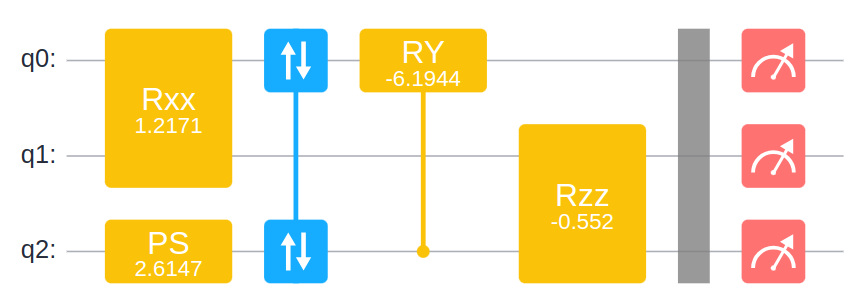
\includegraphics[width=0.9\linewidth]{images/2_6_sampling_circ.png}
    \end{center}
    \caption{采样线路}
\end{figure}

\begin{figure}[h]
    \begin{center}
        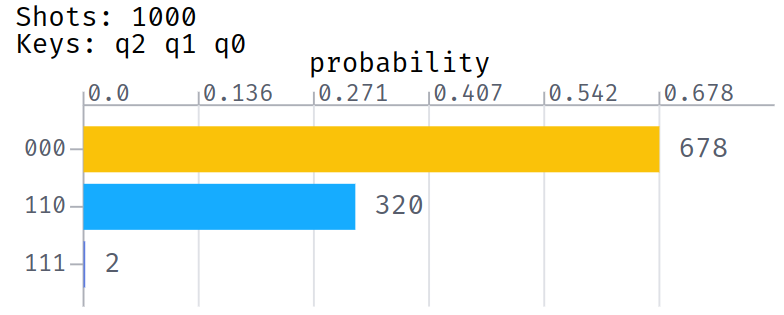
\includegraphics[width=0.9\linewidth]{images/2_6_sampling_res.png}
    \end{center}
    \caption{采样结果}
\end{figure}



\section{量子线路模拟后端}
\label{sec:backend}

\subsection{状态矢量模拟器}
\label{sec_state_vec}
\subsubsection{基于策略的设计模式}
在 \MindQuantum\ 中，我们使用 \Simulator\ 模拟量子态。\Simulator\ 会维护一个量子态；如第 \ref{sec:sim_basic_usage} 节所述，以 \code{apply} 开头的方法会改变该量子态，而以 \code{get} 开头的方法不会改变任何内容，只会从量子态中提取信息。

量子系统模拟对模拟器提出了很高的性能要求。在 \MindQuantum\ 中，我们使用 C++ 或 CUDA 作为底层模拟器实现语言，并基于不同硬件指令集加速量子模拟。我们采用基于策略的开发方式，针对不同指令集优化基础模拟器接口，并将其封装为策略类型。在统一量子模拟框架之上，我们使用不同模拟器策略生成不同量子模拟器，例如支持 AVX 的模拟器、支持 NEON 的模拟器以及支持 GPU 的模拟器。

\begin{figure}[ht]
    \centering
    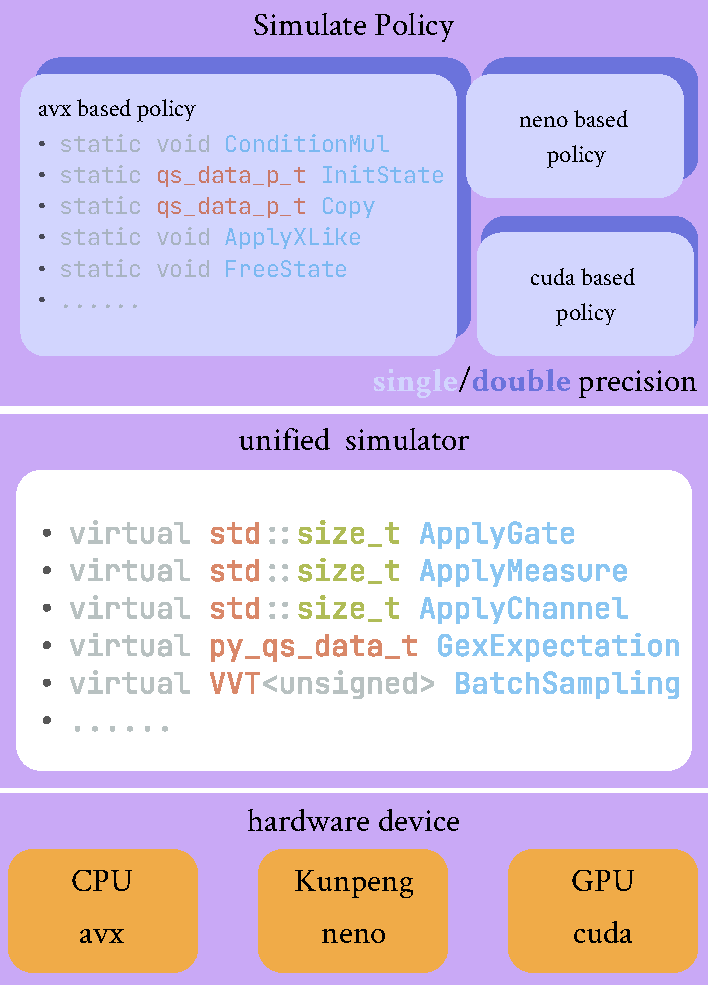
\includegraphics[scale=0.6]{./images/3_1_simulator_structure.pdf}
    \captionsetup{justification=raggedright,singlelinecheck=false}
    \caption{\label{3_1_sim_str} 模拟器的层级结构。\textit{simulate policy} 层根据当前模拟硬件将量子门作用到量子态上。\textit{unified simulator} 层使用不同策略完成线路模拟、期望值计算和梯度计算。\textit{hardware device} 层展示了我们对 CPU、GPU 和鲲鹏平台的支持。}
\end{figure}

根据所模拟的具体量子系统，可以选择全振幅量子模拟器或密度矩阵模拟器。在 \MindQuantum\ 中，这两种模拟器分别称为 \code{"mqvector"} 和 \code{"mqmatrix"}。在当前 \version\ 版本中，\code{"mqvector"} 模拟器也支持 GPU 加速，并命名为 \code{"mqvector_gpu"}。\code{"mqvector"} 和 \code{"mqmatrix"} 都采用图~\ref{3_1_sim_str} 所示的相同设计模式。基于这些模拟器，还可以借助量子信道支持噪声模拟，这将在第~\ref{sec:noise_simulation} 节中讨论。

\subsubsection{基于 SIMD 的量子门优化}
SIMD（Single Instruction Multiple Data，单指令多数据）是一种计算机架构和并行处理技术，旨在通过同时对多个数据元素施加同一操作，加速可并行化任务的执行。量子模拟器的基本构件是量子门与量子态之间的相互作用，其中涉及大量并行操作，因此可以利用 SIMD 提升量子模拟速度。本节将展示如何在 \code{complex128} 数据类型下，基于 AVX 指令优化量子门演化。

AVX 指令提供 256 位宽的向量寄存器，可存储 4 个双精度实数或 2 个双精度复数。在图~\ref{fig:avx} 中，我们以二量子比特全状态矢量为例，概率振幅 $a$ 和 $b$ 可以同时加载到一个 256 位寄存器中，$c$ 和 $d$ 也可以同样处理。
\begin{figure}
    \begin{tikzpicture}[scale=0.5]
        \node[left] at (0,0.5) {256 位寄存器};
        \draw[line width=1.2] (0,0) rectangle (1, 1);
        \draw[line width=1.2] (1,0) rectangle (2, 1);
        \draw[line width=1.2] (2,0) rectangle (3, 1);
        \draw[fill=black] (3.6, 0.5) circle (0.1);
        \draw[fill=black] (4.0, 0.5) circle (0.1);
        \draw[fill=black] (4.4, 0.5) circle (0.1);
        \draw[line width=1.2] (5,0) rectangle (6, 1);
        \draw[line width=1.2] (6,0) rectangle (7, 1);
        \draw[line width=1.2] (7,0) rectangle (8, 1);
        \node[left] at (0,-1) {寄存器 a};
        \draw[line width=1.2] (0,-1.5) rectangle (2, -0.5);
        \draw[line width=1.2] (2,-1.5) rectangle (4, -0.5);
        \draw[line width=1.2] (4,-1.5) rectangle (6, -0.5);
        \draw[line width=1.2] (6,-1.5) rectangle (8, -0.5);
        \node at (1,-1) {$b_i$};
        \node at (3,-1) {$b_r$};
        \node at (5,-1) {$a_i$};
        \node at (7,-1) {$a_r$};
        \node[left] at (0,-2.5) {寄存器 b};
        \draw[line width=1.2] (0,-3) rectangle (2, -2);
        \draw[line width=1.2] (2,-3) rectangle (4, -2);
        \draw[line width=1.2] (4,-3) rectangle (6, -2);
        \draw[line width=1.2] (6,-3) rectangle (8, -2);
        \node at (1,-2.5) {$d_i$};
        \node at (3,-2.5) {$d_r$};
        \node at (5,-2.5) {$c_i$};
        \node at (7,-2.5) {$c_r$};
        \draw[dashed, line width=1.2, fill=red!50] (8, -0.5) -- (8, -1.5) -- (10, -1.4) -- (12, -1.4) -- (12, 0.5) -- (10, 0.5) -- cycle;
        \draw[dashed, line width=1.2, fill=blue!50] (8, -2) -- (8, -3) -- (10, -3.4) -- (12, -3.4) -- (12, -1.6) -- (10, -1.6) -- cycle;
        \node[right] at (9, 1) {$\ket{\psi}=$};
        \node[right] at (9.5, -0) {$a\ket{00}+$};
        \node[right] at (9.5, -1) {$b\ket{01}+$};
        \node[right] at (9.5, -2) {$c\ket{10}+$};
        \node[right] at (9.5, -3) {$d\ket{11}$};
    \end{tikzpicture}
    \caption{将二量子比特量子态存储到两个 256 位寄存器中。}
    \label{fig:avx}
\end{figure}

我们将基本量子门划分为不同类型，例如类 X 门、类 Z 门或矩阵门。对于类 X 门，矩阵元素仅位于反对角线上：
\begin{equation}
    \begin{pmatrix}
        0 & a \\
        b & 0
    \end{pmatrix}.
\end{equation}
当类 X 门作用在第一个量子比特上时，需要在单个 AVX 寄存器中交换 $(b*a_r, b*a_i)$ 和 $(a*b_r, a*b_i)$。如果该门作用在其他量子比特上，则需要交换 $b*\text{reg\_a}$ 和 $a*\text{reg\_b}$。对于类 Z 门，矩阵元素仅位于对角线上：
\begin{equation}
    \begin{pmatrix}
        a & 0 \\
        0 & b
    \end{pmatrix}.
\end{equation}
在这种情况下，如果量子门作用在第一个量子比特上，只需将 $(a_r, a_i)$ 改为 $(a*a_r, a*a_i)$，并将 $(b_r, b_i)$ 改为 $(b*b_r, b*b_i)$；如果作用在其他量子比特上，则只需让寄存器 a 乘以 $a$，寄存器 b 乘以 $b$。

\subsection{密度矩阵模拟器}
不同于状态矢量模拟器，密度矩阵模拟器更适合混态或开放量子系统模拟，但内存消耗也大得多。量子系统的密度算符描述为：
\begin{equation}
    \rho=\sum_ip_i\ket{\psi_i}\bra{\psi_i},
\end{equation}
其中，$p_i$ 是系统处于纯态 $\ket{\psi_i}$ 的概率。量子门 $U$ 对密度算符的演化为：
\begin{equation}
    \rho'=U\rho U^\dagger.
\end{equation}
可观测量 $H$ 在 $\rho$ 下的期望值为：
\begin{equation}
    \left<H\right> = \sum_ip_i\bra{\psi_i}H\ket{\psi_i}=\tr(\rho H).
\end{equation}

其使用方法、开发策略和优化流程都与状态矢量模拟器非常相似，请参见第~\ref{sec_state_vec} 节。


\subsection{量子化学 CI 子空间模拟器}
\label{sec:mqchem}
\texttt{mqchem} 是 \MindQuantum\ 中面向量子化学问题的专用模拟模块。与通用状态矢量模拟器不同，它不在完整的 $2^{n_q}$ 维计算基上保存量子态，而是在固定电子数的配置相互作用（Configuration Interaction, CI）子空间中演化波函数。这里 $n_q$ 表示自旋轨道数，也对应量子比特数；若体系含有 $n_e$ 个电子，则 CI 空间维度为
\begin{equation}
    \dim \mathcal{H}_{\mathrm{CI}}(n_q,n_e)=\binom{n_q}{n_e}.
\end{equation}
对于电子数远小于完整 Fock 空间的分子体系，这一表示通常比全振幅状态矢量更加紧凑。若 ansatz 进一步采用保持自旋的 singlet UCCSD 激发，演化还会停留在由这些激发确定的物理扇区内；这一约束来自激发算符和 ansatz 的选择，而 \texttt{mqchem} 后端本身以固定电子数 CI 基为核心索引。

\texttt{mqchem} 的底层状态可理解为 Slater 行列式振幅组成的 CI 向量。实现中，每个行列式由一个整数 bitmask 表示，置位的自旋轨道表示被电子占据；后端通过组合数索引在 bitmask 与紧凑数组下标之间转换，并按 $(n_q,n_e)$ 缓存索引器。模拟器默认从 Hartree-Fock 参考态开始，即最低的 $n_e$ 个自旋轨道被占据。用户也可以用稀疏表示设置态矢量，其中每一项给出一个占据 bitmask 及其振幅；不满足固定电子数条件的基态会被拒绝。

该模块围绕三类对象组织。首先，\texttt{MQChemSimulator} 负责保存 CI 向量、施加 UCC 激发线路、计算期望值和生成梯度函数。其次，\texttt{CIHamiltonian} 将实系数费米子哈密顿量封装成适用于 CI 空间的哈密顿量对象，并在内部预处理产生湮灭掩码、产生掩码、翻转掩码和费米子奇偶相位信息。最后，\texttt{UCCExcitationGate} 将单项 \texttt{FermionOperator} 表示的激发算符 $\hat{T}$ 封装为
\begin{equation}
    \hat{U}(\theta)=\exp\left[\theta\left(\hat{T}-\hat{T}^{\dagger}\right)\right],
\end{equation}
用于构造 UCC 类型的变分线路。该门专门配合 \texttt{MQChemSimulator} 使用，并不等价于通用状态矢量模拟器中的普通量子门。

对于常见的单激发和双激发，\texttt{mqchem} 不需要显式构造完整矩阵。给定一组满足激发条件的行列式对 $\{\ket{i},\ket{j}\}$，激发门只在这二维子空间中做旋转。若 $s_{ij}=\pm1$ 表示费米子反对易关系带来的奇偶相位，则振幅更新可写为
\begin{equation}
    \begin{pmatrix}
        c_i' \\
        c_j'
    \end{pmatrix}
    =
    \begin{pmatrix}
        \cos\theta       & -s_{ij}\sin\theta \\
        s_{ij}\sin\theta & \cos\theta
    \end{pmatrix}
    \begin{pmatrix}
        c_i \\
        c_j
    \end{pmatrix}.
\end{equation}
实现会为激发门预先计算活跃轨道掩码、态对识别掩码、翻转掩码和每个费米子算符对应的奇偶掩码。实际演化时，只需扫描 CI 向量中的基态并更新被同一激发连接的振幅对。哈密顿量作用也采用类似思路：逐项检查湮灭算符要求的占据条件和产生算符要求的空占条件，计算费米子相位，再把输入行列式映射到输出行列式。由此，期望值 $\langle\psi|\hat{H}|\psi\rangle$ 可直接在 CI 向量上求得。

面向 VQE 训练时，\texttt{MQChemSimulator} 的梯度接口会返回一个可调用对象，一次前向计算即可给出能量期望值及其关于 UCC 参数的梯度。底层采用伴随反传思路：先正向施加参数化激发线路，再通过反向线路和哈密顿量作用计算各个参数的贡献；对单个 UCC 激发门的导数，后端仍利用上述二维耦合结构直接求值，避免构造大矩阵或进行有限差分。

下面的代码展示了 \texttt{mqchem} 在 UCCSD-VQE 中的典型使用方式。与前文使用 \texttt{Simulator("mqvector", ...)} 的流程相比，这里不需要先把 UCC 激发全部展开成 Pauli 字符串演化线路，而是直接在费米子占据基中构造 ansatz、哈密顿量和初始参数。
\begin{lstlisting}
from mindquantum.simulator import mqchem

ham, circ, init_amp = mqchem.prepare_uccsd_vqe(
    molecule,
    threshold=1e-6,
)

sim = mqchem.MQChemSimulator(
    molecule.n_qubits,
    molecule.n_electrons,
    dtype="double",
)
grad_ops = sim.get_expectation_with_grad(ham, circ)

energy, gradient = grad_ops(init_amp)
\end{lstlisting}

\texttt{prepare\_uccsd\_vqe} 是该模块提供的高层辅助接口。它会从分子对象中读取二次量子化哈密顿量并生成 \texttt{CIHamiltonian}，调用 \texttt{uccsd\_singlet\_generator} 产生 singlet UCCSD 激发，读取已计算的 CCSD 单、双激发振幅作为初始猜测，并根据给定阈值过滤幅度很小的激发项。若用户需要构造分层或 Trotter 化的 UCC ansatz，\texttt{SequentialUCCAnsatz} 还允许按照插入顺序逐项追加激发算符，即使同一激发在不同层中以不同参数重复出现也会被保留。

\texttt{mqchem} 因而更适合作为量子化学算法研究和 VQE 数值实验的专用后端：它保留了费米子占据数和 UCC 激发结构中的物理信息，减少了中间 Pauli 展开带来的模拟开销；而当目标是在真实量子芯片上执行线路时，仍应使用前文介绍的费米子到量子比特映射、量子线路 ansatz 和编译流程。


\subsection{基于信道的噪声模拟器}
\label{sec:noise_simulation}

查看本节演示代码：\demonotebook{03}{chapt03} \ \demonotebookgithub{03}{chapt03}

\subsubsection{量子信道}
由于量子退相干以及与环境的耦合，当前量子计算机在计算过程中经常发生误差。这些误差会出现在态制备、量子门操作和测量等阶段，通常称为量子噪声。量子噪声可以由量子信道刻画。在量子信息理论中，量子信道是指算符空间中的完全正定保迹（CPTP）映射，也可视为一种量子操作。所有量子信道都可以由 Kraus 算符表示：

\begin{equation}
    \Psi(\rho) = \sum_i K_i \rho K_i^\dagger,
\end{equation}

其中，$\Psi$ 为量子信道，$\rho$ 为密度矩阵，$\{K_i\}$ 为 $\Psi$ 的 Kraus 算符。Kraus 算符满足完备性条件：

\begin{equation}
    \sum_i K_i^\dagger K_i = I.
\end{equation}

在密度矩阵模拟器 \code{"mqmatrix"} 中，我们支持基于上述数学形式模拟量子信道。除密度矩阵方法外，在 \MindQuantum\ 的状态矢量模拟器 \code{"mqvector"} 中，我们也支持使用 Monte Carlo 方法模拟量子信道。噪声门会以一定概率影响量子比特。通过对线路进行多次采样，可以得到包含噪声的量子线路模拟结果。这个过程更加接近真实量子计算机的工作方式。

\MindQuantum\ 中实现了以下量子信道。

\PauliChannel：Pauli 信道可以看作 Pauli 算符按照某一概率分布随机作用于量子态 $\rho$。
\begin{equation}
    \Psi(\rho) = (1-p_x-p_y-p_z) \rho + p_x X \rho X + p_y Y \rho Y + p_z Z \rho Z.
\end{equation}
如果只有 $p_x$ 非零，它就成为 \BitFlipChannel。类似地，\PhaseFlipChannel\ 只有 $p_z$ 一个非零值，而 \BitPhaseFlipChannel\ 中非零的是 $p_y$。一个特殊情形是所有 Pauli 算符具有相同概率，这称为 \DepolarizingChannel。退极化信道广泛用于描述量子噪声。以下是一量子比特情形下的公式：
\begin{equation}
    \Psi(\rho) =  (1-p) \rho + \frac{p}{4}(I\rho I+X\rho X+Y\rho Y+Z\rho Z).
\end{equation}
\MindQuantum\ 中的退极化信道也支持多量子比特情形。
\begin{lstlisting}
from mindquantum.core.gates import DepolarizingChannel
from mindquantum.core.circuit import Circuit
circ = Circuit()
circ += DepolarizingChannel(0.02).on(0)
circ += DepolarizingChannel(0.01, 2).on([0, 1])
\end{lstlisting}

阻尼信道：常见的阻尼信道包括 \AmplitudeDampingChannel\ 和 \PhaseDampingChannel。振幅阻尼信道可以描述系统能量耗散，而相位阻尼信道描述的是不与环境交换能量时量子信息的损失。
振幅阻尼信道施加噪声的形式为：
\begin{gather*}
    \epsilon(\rho) = E_0 \rho E_0^\dagger + E_1 \rho E_1^\dagger
    \\
    \text{其中}\ {E_0}=\begin{bmatrix}1 & 0               \\
        0 & \sqrt{1-\gamma}\end{bmatrix},
    \ {E_1}=\begin{bmatrix}0 & \sqrt{\gamma} \\
        0 & 0\end{bmatrix}.
\end{gather*}
相位阻尼信道施加噪声的形式为：
\begin{gather*}
    \epsilon(\rho) = E_0 \rho E_0^\dagger + E_1 \rho E_1^\dagger
    \\
    \text{其中}\ {E_0}=\begin{bmatrix}1 & 0               \\
        0 & \sqrt{1-\gamma}\end{bmatrix},
    \ {E_1}=\begin{bmatrix}0 & 0             \\
        0 & \sqrt{\gamma}\end{bmatrix}.
\end{gather*}

\KrausChannel：这是 \MindQuantum\ 中的自定义单量子比特量子信道，可以通过传入 Kraus 算符构造。
\begin{lstlisting}
from mindquantum.core.gates import KrausChannel
from mindquantum.core.circuit import Circuit
from cmath import sqrt
gamma = 0.5
kmat0 = [[1, 0], [0, sqrt(1 - gamma)]]
kmat1 = [[0, sqrt(gamma)], [0, 0]]
amplitude_damping = KrausChannel('damping', [kmat0, kmat1])
circ = Circuit()
circ += amplitude_damping.on(0)
\end{lstlisting}

\subsubsection{Channel Adder}
真实量子芯片由多个量子比特组成。由于制造过程中的固有差异，每个量子比特都会表现出不同误差来源。此外，即使是同一个量子比特，在施加不同量子门时对应误差也会发生变化。为了忠实复现量子芯片中的固有误差，需要精心设计精确的误差模型。在 \MindQuantum\ 中，我们开发了一组名为 Channel Adder（信道添加器）的工具，用于快速构建噪声模型。通过 Channel Adder，可以方便地在不同量子门之后引入不同量子信道，并针对特定量子比特进行定制，再利用含噪模拟器模拟这些噪声模型。

\ChannelAdder\ 类主要由三个函数组成：\code{_accepter()}、\code{_excluder()} 和 \code{_handler(BasicGate)}。它们的功能如下：
\begin{itemize}
    \item \code{_accepter()}：返回一个函数列表，称为接受规则集；其中每个接受规则函数都以量子门作为输入。当函数返回 True 时，表示可以在该量子门之后添加信道。
    \item \code{_excluder()}：返回一个函数列表，称为拒绝规则集；其中每个拒绝规则函数都以量子门作为输入。当函数返回 True 时，表示拒绝在该量子门之后添加信道。
    \item \code{_handler(BasicGate)}：以量子门作为输入，并返回一个量子线路，用于表示添加在输入量子门之后的自定义信道。
\end{itemize}

以 \BitFlipAdder\ 为例。该添加器会在每个量子门之后添加一个比特翻转信道。
\begin{lstlisting}
from mindquantum.core.circuit import Circuit, BitFlipAdder

circ = Circuit().h(0).rx('a', 1).z(1, 0)
noise_model = BitFlipAdder(0.3, with_ctrl=False)
noise_circ = noise_model(circ)
print(noise_model)
\end{lstlisting}
输出为：
\begin{lstlisting}
BitFlipAdder<flip_rate=0.3, with_ctrl=False>
\end{lstlisting}
将该噪声模型应用到线路后，每个量子门之后都会添加一个比特翻转信道，如图~\ref{fig:bit_flip_adder} 所示。
\begin{figure}
    \centering
    \begin{subfigure}{0.2\textwidth}
        \centering
        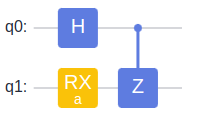
\includegraphics[width=\textwidth]{images/3_3_no_bit_fip.png}
        \caption{无噪声线路。}
    \end{subfigure}
    \begin{subfigure}{0.4\textwidth}
        \centering
        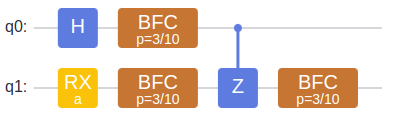
\includegraphics[width=0.9\textwidth]{images/3_3_bit_fip.png}
        \caption{经过 \texttt{BitFlipAdder} 处理后的线路。}
    \end{subfigure}
    \caption{将 BitFlipAdder 应用于量子线路的示例。}
    \label{fig:bit_flip_adder}
\end{figure}

下面给出一个更复杂的示例，以展示 Channel Adder 的能力。假设量子芯片上不同量子比特的单量子比特门操作噪声可以忽略不计，并考虑两量子比特门在不同量子比特上表现出不同的退极化信道。此外，线路测量会受到比特翻转误差影响，翻转概率为 0.01。假设不同量子比特上的退极化信道为：
\begin{lstlisting}
from mindquantum.core import *
dc0 = DepolarizingChannel(0.01)
dc1 = DepolarizingChannel(0.02)
dc2 = DepolarizingChannel(0.03)
\end{lstlisting}
接下来按如下方式构建完整噪声模型：
\begin{lstlisting}
adder1 = MixerAdder([
    NoiseExcluder(),
    ReverseAdder(MeasureAccepter()),
    QubitNumberConstrain(2),
    NoiseChannelAdder(dc0, focus_on=0),
])
adder2 = MixerAdder([
    NoiseExcluder(),
    ReverseAdder(MeasureAccepter()),
    QubitNumberConstrain(2),
    NoiseChannelAdder(dc1, focus_on=1),
])
adder3 = MixerAdder([
    NoiseExcluder(),
    ReverseAdder(MeasureAccepter()),
    QubitNumberConstrain(2),
    NoiseChannelAdder(dc2, focus_on=2),
])
adder4 = MixerAdder([
    NoiseExcluder(),
    MeasureAccepter(),
    BitFlipAdder(0.01)
], add_after=False)

noise_model = SequentialAdder([
    adder1,
    adder2,
    adder3,
    adder4
])
print(noise_model)
\end{lstlisting}
输出为：
\begin{lstlisting}
SequentialAdder<
  MixerAdder<
    NoiseExcluder<>
    ReverseAdder<
      MeasureAccepter<>
    >
    QubitNumberConstrain<n_qubits=2, with_ctrl=True>
    NoiseChannelAdder<channel=DC(p=1/100), with_ctrl=True>
  >
  MixerAdder<
    NoiseExcluder<>
    ReverseAdder<
      MeasureAccepter<>
    >
    QubitNumberConstrain<n_qubits=2, with_ctrl=True>
    NoiseChannelAdder<channel=DC(p=1/50), with_ctrl=True>
  >
  MixerAdder<
    NoiseExcluder<>
    ReverseAdder<
      MeasureAccepter<>
    >
    QubitNumberConstrain<n_qubits=2, with_ctrl=True>
    NoiseChannelAdder<channel=DC(p=0.03), with_ctrl=True>
  >
  MixerAdder<
    NoiseExcluder<>
    MeasureAccepter<>
    BitFlipAdder<flip_rate=0.01, with_ctrl=True>
  >
>
\end{lstlisting}
\MixerAdder\ 是一组添加器，只有满足所有 \code{_accepter()} 和 \code{_excluder()} 规则时才会生效。\SequentialAdder\ 中的所有 Channel Adder 会逐一执行。从图~\ref{fig:complex_adder} 可以看出，该噪声模型满足我们的需求。

% \begin{lstlisting}
% circ = Circuit().rx('a', 0).rx('b', 1).x(1, 0).rz('c', 1).x(1, 0).measure_all()
% \end{lstlisting}
\begin{figure}
    \centering
    \begin{subfigure}{0.32\textwidth}
        \centering
        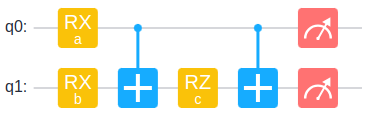
\includegraphics[width=\textwidth]{images/3_3_no_complex.png}
        \caption{无噪声线路。}
    \end{subfigure}
    \begin{subfigure}{0.5\textwidth}
        \centering
        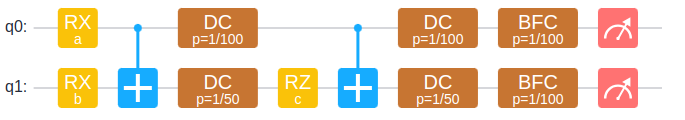
\includegraphics[width=\textwidth]{images/3_3_complex.png}
        \caption{经过复合 Channel Adder 处理后的线路。}
    \end{subfigure}
    \caption{将复合 Channel Adder 应用于量子线路的示例。}
    \label{fig:complex_adder}
\end{figure}

构建噪声模型后，可以在 \MindQuantum\ 中很方便地使用该噪声模型模拟量子线路。
\begin{lstlisting}
circ = Circuit().rx('a', 0).rx('b', 1).x(1, 0).rz('c', 1).x(1, 0).measure_all()
noise_sim = Simulator(NoiseBackend('mqvector', 2, noise_model))
noise_sim.sampling(circ, pr={'a': 1, 'b': 2, 'c':3}, shots=10000)
\end{lstlisting}
这里，我们使用基于 \code{"mqvector"} 的 \NoiseBackend\ 和此前构建的噪声模型，构造了一个噪声模拟器。


\section{MindSpore Quantum 工具箱}
\label{sec:toolbox}

查看本章演示代码：\demonotebook{04}{chapt04} \ \demonotebookgithub{04}{chapt04}

\subsection{变分量子算法的梯度}
得益于量子叠加、量子纠缠和量子并行性等原理，量子算法能够高效处理某些计算问题，例如 Shor 算法 \cite{shor1994algorithms}、Grover 算法 \cite{grover1996fast,long2001grover} 和 Harrow-Hassidim-Lloyd 算法 \cite{harrow2009quantum}，并相较经典算法实现指数级或多项式级加速。然而，当前阶段的量子设备仍受限于量子比特数量有限和显著噪声，通常称为含噪中等规模量子（NISQ）设备 \cite{preskill2018quantum}。需要注意的是，上述量子算法在 NISQ 时代并不表现出量子优势。

变分量子算法（Variational Quantum Algorithms, VQA）\cite{cerezo2021variational,yuan2019theory,xu2021variational} 被认为是 NISQ 时代实现量子优势最有希望的候选方案。VQA 利用经典机器学习中的优化算法，对参数化量子线路（Parameterized Quantum Circuit, PQC）进行调优。因此，VQA 是一种量子-经典混合算法。VQA 已广泛应用于多个领域，包括量子多体模拟 \cite{Peruzzo2014Peruzzo2014,kandala2017hardware,kokail2019self,lyu2023variational,Lyu2023symmetryenhanced,cao2022progress}、量子近似优化算法 \cite{farhi2014quantum,patti2022variational,chandarana2023digitized}、量子机器学习 \cite{benedetti2019parameterized,wei2022quantum,lloyd2018quantum,biamonte2017quantum,abbas2021power} 和纠缠纯化 \cite{zhang2023variational}。本节将简要概述 VQA 算法的工作流程，以及如何在 \MindQuantum\ 中高效实现该流程。更多 VQA 算法应用示例将在第 \ref{sec:applications} 章中展示。

\begin{figure}[h]
  \begin{center}
    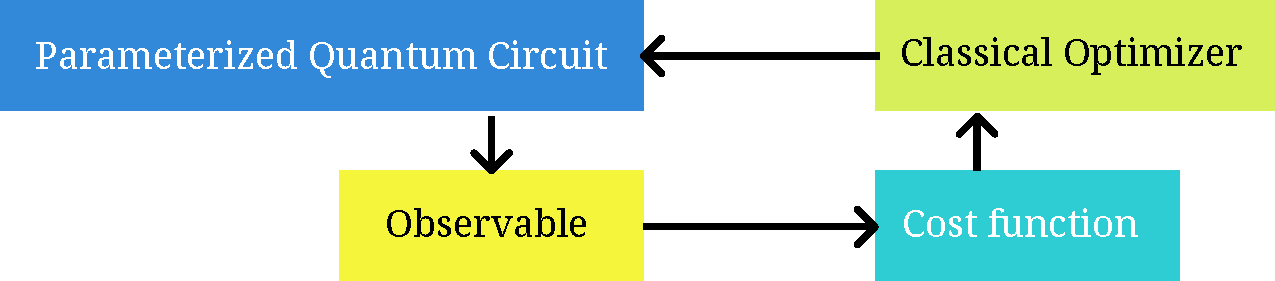
\includegraphics[width=0.9\linewidth]{images/4_1_vqa.pdf}
  \end{center}
  \caption{VQA 的工作流程。}
  \label{fig:vqa_work_flow}
\end{figure}

图~\ref{fig:vqa_work_flow} 展示了 VQA 的主要工作流程。VQA 的核心组成部分是 PQC，其中既包含 Hadamard 门和 Pauli 门等非参数化量子门，也包含绕 Bloch 球 $x$、$y$ 或 $z$ 轴旋转的参数化量子门。根据具体任务，PQC 可以分为两部分：编码器线路负责将经典数据编码为量子态，记为 $U_e(\alpha)$；ansatz 线路则作为 VQA 中可训练的部分，记为 $U_a(\theta)$。

在 VQA 中，还需要一个记为 $H$ 的可观测算符。该可观测量的期望值计算如下：

\begin{equation}
  E(\alpha, \theta) = \bra{0}U_e^\dagger(\alpha)U_a^\dagger(\theta)HU_a(\theta)U_e(\alpha)\ket{0}.
\end{equation}
在量子多体模拟和量子近似优化算法中，需要将问题转换为可观测量，并优化参数 $\theta$ 以寻找该可观测量的基态（在这类问题中，编码器线路 $U_e$ 通常为恒等）。该任务可描述为：

\begin{equation}
  \min_\theta E(\theta).
\end{equation}
另一方面，当将 VQA 作为机器学习模型的一部分时，需要定义代价函数：

\begin{equation}
  \min_\theta L(E(\alpha, \theta), E_\text{target}),
\end{equation}
其中，$E_\text{target}$ 是训练模型的目标值，$L$ 是代价函数，例如平均绝对误差损失或均方误差损失。

VQA 中的优化算法可以根据是否依赖梯度分为两类。第一类是基于梯度的优化算法，例如 Adam 和 BFGS。这类算法非常适合在量子模拟器中实现。第二类是不基于梯度的优化算法，例如 SPSA 和 Nelder-Mead。这类算法在真实量子实验中更具实用性。在 \MindQuantum\ 中，我们主要关注基于梯度的优化器，并将在第 \ref{sec:benchmark} 节中进一步说明如何加速 PQC 梯度计算。

\subsubsection{学习一个旋转}

本小节将通过一个学习旋转量子门的任务，深入介绍如何在 \MindQuantum\ 中实现变分量子算法。

假设初始量子态为 $\ket{\psi_0}=\ket{0}$，我们的目标是寻找一个单量子比特酉算符 $U(\theta)$，将 $\ket{\psi_0}$ 旋转到 $\ket{\psi_f}$，并使 $E_X(\theta) = \bra{\psi_f}X\ket{\psi_f}$ 最小：

\begin{equation}
  \min_\theta(\bra{0}U^\dagger(\theta)XU(\theta)\ket{0}).
\end{equation}

VQA 的第一步是构建 ansatz。在该任务中，我们选择任意单量子比特旋转门 \Uthree\ 作为 ansatz；\Uthree\ 也可以分解为：

\begin{equation}
  U_3(a, b, c) = RZ(b)RX(-\pi/2)RZ(a)RX(\pi/2)RZ(c).
\end{equation}

\begin{lstlisting}
import numpy as np
from mindquantum.core.circuit import Circuit

ansatz = Circuit().rz('c', 0).rx(np.pi/2, 0)
ansatz.rz('a', 0).rx(-np.pi/2, 0).rz('b', 0)
ansatz.svg()
\end{lstlisting}

\begin{figure}[h]
  \begin{center}
    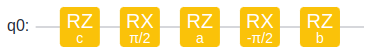
\includegraphics[width=0.9\linewidth]{images/4_1_ansatz.png}
  \end{center}
  \caption{可作为任意单量子比特旋转的 ansatz 线路。}
  \label{fig:u3_ansatz}
\end{figure}

可观测量实现如下：

\begin{lstlisting}
from mindquantum.core.operators import QubitOperator
from mindquantum.core.operators import Hamiltonian

obs = QubitOperator('X0')
ham = Hamiltonian(obs)
\end{lstlisting}

在 \MindQuantum\ 中，模拟器提供了 \getexpectationwithgrad\ 方法，可方便地计算 $E_X(\theta)$ 的梯度。

\begin{lstlisting}
import numpy as np
from mindquantum.simulator import Simulator

sim = Simulator('mqvector', ansatz.n_qubits)
grad_ops = sim.get_expectation_with_grad(ham, ansatz)

p0 = np.random.uniform(-np.pi, np.pi, len(ansatz.params_name))
f, g = grad_ops(p0)
print(f, g)
\end{lstlisting}
输出为：
\begin{lstlisting}
[[-0.04602095+0.j]] [[[-1.17340357e-17+0.j -3.47310364e-02+0.j -7.96875999e-01+0.j]]]
\end{lstlisting}

\getexpectationwithgrad\ 接收可观测量哈密顿量和 ansatz 线路，并返回一个梯度算符。可以使用该算符在任意 ansatz 参数处计算梯度。梯度算符的输出包含期望值及其关于 ansatz 参数的梯度。期望值的形状为 $[n_\text{batch}, n_\text{ham}]$，其中 $n_\text{batch}$ 是编码器数据的批大小，$n_\text{ham}$ 是哈密顿量数量。在该任务中，我们没有编码器，且只有一个可观测量，因此 $n_\text{batch}=1, n_\text{ham}=1$。ansatz 梯度的形状为 $[n_\text{batch}, n_\text{ham}, n_\text{ansatz}]$，其中 $n_\text{ansatz} = 3$ 是 ansatz 线路中的参数数量。

下一步是借助梯度算符优化 PQC。
\begin{lstlisting}
from scipy.optimize import minimize

def fun(p0, grad):
  f, g = grad(p0)
  f = np.real(f)[0, 0]
  g = np.real(g)[0, 0]
  return f, g

res = minimize(fun, p0, method='bfgs', jac=True, args=(grad_ops, ))
print('min E:', res.fun)
print('Best p:', res.x)
\end{lstlisting}
可以得到最小化后的可观测量取值以及对应的 ansatz 参数：
\begin{lstlisting}
min E: -0.9999999999994561
Best p: [-2.51566965 -4.71238798 -3.14159296]
\end{lstlisting}
因此，学习得到的旋转为：
\begin{lstlisting}
ansatz.matrix(pr=dict(zip(ansatz.params_name, res.x)))
\end{lstlisting}
\begin{align*}
  U_a=\frac{1}{\sqrt{2}}\begin{pmatrix}
    e^{-0.313i}  & e^{0.313i} \\
    -e^{-0.313i} & e^{0.313i}
  \end{pmatrix}.
\end{align*}

\subsubsection{旋转三个态}
\label{sec:rotate_three_states}

在前一个示例中，PQC 只包含 ansatz 线路；在本示例中，我们将展示如何在 \MindQuantum\ 中向 PQC 加入编码器线路。问题描述如下：寻找一个单量子比特旋转门 $U_a(\theta)$，使以下三个态的 $Z$ 期望值之和最大：$\ket{\psi_0}=\ket{0},\ket{\psi_1}=(\ket{0}+\ket{1})/\sqrt{2}$ 和 $\ket{\psi_2}=(\ket{0}+i\ket{1})/\sqrt{2}$。

\begin{equation}
  \max_{\theta}\sum_i{\bra{\psi_i}U^\dagger(\theta)ZU(\theta)\ket{\psi_i}}.
\end{equation}

这里，我们使用编码器线路 $U_e(a, b) = RX(a)RY(b)$ 制备态 $\ket{\psi_i}=U_e(a, b)\ket{0}$：
\begin{lstlisting}
import numpy as np
from mindquantum.core.circuit import Circuit

encoder = Circuit().rx('a', 0).ry('b', 0)
encoder = encoder.as_encoder()

e_data = np.array([[0.0, 0.0],      # psi_0
                   [0.0, np.pi/2],  # psi_1
                   [-np.pi/2, 0.0], # psi_2
                  ])
\end{lstlisting}
在上述代码中，我们调用 \asencoder\ 将量子线路转换为编码器线路。在本示例中，我们将展示如何借助 MindSpore 机器学习框架训练 PQC。

\begin{lstlisting}
# 构建任意单量子比特旋转 ansatz
from mindquantum.framework import MQLayer
import mindspore.nn as nn
import mindspore as ms

ansatz = Circuit().rz('a2', 0).rx(np.pi/2, 0)
ansatz.rz('a0', 0).rx(-np.pi/2, 0).rz('a1', 0)

obs = QubitOperator('Z0')
ham = Hamiltonian(-obs)

sim = Simulator('mqvector', 1)
total_circ = encoder + ansatz
grad_ops = sim.get_expectation_with_grad(ham, total_circ)

e_tensor = ms.Tensor(e_data, ms.float32)

quantum_net = MQLayer(grad_ops)

class Hybrid(nn.Cell):
    def __init__(self, quantum_net):
        super(Hybrid, self).__init__()
        self.quantum_net = quantum_net
    def construct(self, e):
        x = self.quantum_net(e)
        x = x.sum()
        return x

hybrid = Hybrid(quantum_net)
opti = nn.Adam(quantum_net.trainable_params(), learning_rate=0.1)
train_net = nn.TrainOneStepCell(hybrid, opti)
for step in range(100):
    print(-train_net(e_tensor))
\end{lstlisting}
最终学习得到的期望值之和为 1.732。此外，我们还可以在 \MindQuantum\ 中方便地展示这些量子态：

\begin{lstlisting}
import matplotlib.pyplot as plt
from mindquantum.io import BlochScene
from mindquantum.core.parameterresolver import ParameterResolver as PR

e_name = encoder.params_name
a_name = ansatz.params_name
a_data = np.array(quantum_net.weight)

init_states = [encoder.get_qs(pr=dict(zip(e_name, i))) for i in e_data]
final_states = []
for i, data in enumerate(e_data):
    pr = PR(dict(zip(e_name, data)))
    pr += PR(dict(zip(a_name, a_data)))
    final_states.append(total_circ.get_qs(pr=pr))

scene = BlochScene()
fig, ax = scene.create_scene()

for i in init_states:
    scene.add_state(ax,
        i,
        linecolor='r',
        with_proj=False)

for i in final_states:
    scene.add_state(ax,
        i,
        linecolor='g',
        with_proj=False)

plt.show()
\end{lstlisting}

\begin{figure}[ht]
  \centering
  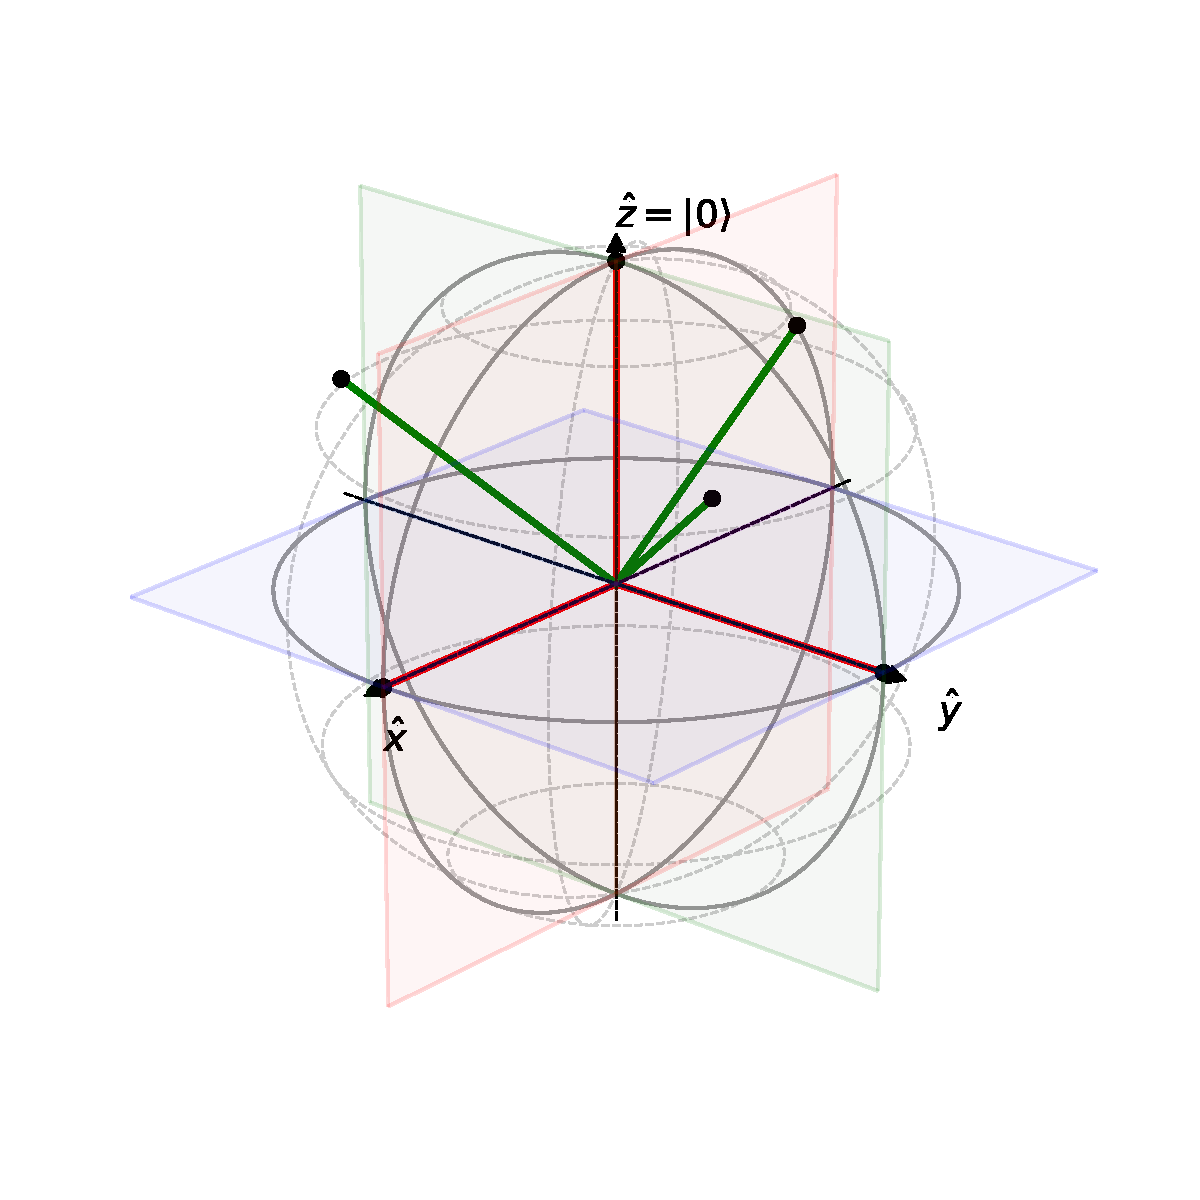
\includegraphics[scale=0.48]{./images/4_1_result.pdf}
  \caption{\label{4_1_vqa} 初始态的旋转。红色表示初始量子态，绿色表示最终量子态。}
\end{figure}

\subsubsection{更多用法}
在 \MindQuantum\ 中，除上述两种基本用法外，\getexpectationwithgrad\ 还提供了更广泛的应用场景。实际计算梯度的表达式定义为：
\begin{equation}
  E = \left<\varphi\right|U_l^\dagger H U_r \left|\psi\right>.
\end{equation}
可以将 $U_l$ 设置为空线路，并将 $H$ 设置为恒等 \QubitOperator，从而得到新态在 $\ket{\varphi}$ 上的投影。也可以设置 $\ket{\varphi}=\ket{\psi}$、$U_l = U_r$，并将 $H$ 设置为密度矩阵，例如 $H = \ket{0}\bra{0}$，此时结果为
\begin{equation}
  E=\left|\bra{0}U_r\ket{\psi}\right|^2.
\end{equation}
还可以将可观测量设置为哈密顿量列表，使 \MindQuantum\ 能够并行计算期望值和梯度。


\subsection{量子线路 Ansatz 库}
Ansatz 是 VQA 中的一个重要术语，本质上是对适合当前问题的量子态形式所作的猜测或假设。例如，在变分量子本征求解器（VQE）中，ansatz 被选择用于表示量子系统的基态或低能态。根据线路结构是预先确定还是在优化过程中动态更新，ansatz 可以是固定的，也可以是自适应的。ansatz 的选择会影响 VQA 的性能和鲁棒性，也会影响量子计算和经典计算所需的资源。因此，选择或设计合适的 ansatz 是 VQA 成功的重要环节。

\MindQuantum\ 的 \nisq\ 模块包含许多常用 ansatz，如下所示。

\begin{itemize}
    \item \IQPEncoding：IQP Encoding 是一种将经典数据编码为量子态的方法 \cite{Havlíček2019}。它使用旋转门和受控门构造量子线路，使输入数据能够由旋转门参数调节，并使输出量子态反映输入数据的特征。IQP Encoding 的一个优势是能够生成高维量子特征空间，从而提升机器学习性能。

    \item \HardwareEfficientAnsatz：这是一类容易在量子芯片上实现的 ansatz \cite{Kandala2017,doi:10.1021/acs.jctc.3c00966}。硬件高效 ansatz 由一层单量子比特旋转门和一层双量子比特纠缠门构造而成。单量子比特旋转门层由作用于每个量子比特的一个或多个旋转门构成；双量子比特纠缠门层则由作用在纠缠映射上的 CNOT、CZ、Rxx、Ryy、Rzz 等量子门构成。

    \item \StronglyEntangling：它通常用于量子机器学习。其优势在于可以到达“希尔伯特空间的广阔区域”\cite{Schuld_2020}，因此被认为非常适合作为分类器的 ansatz。

    \item \MaxCutAnsatz：\MaxCutAnsatz\ 是 QAOA 的一种 ansatz 线路 \cite{farhi2014quantum}，用于求解正则图上的最大割问题。最大割问题是图论中的 NP 完全问题，要求将图的顶点划分为两部分，并最大化被切割边的数量。\MaxCutAnsatz\ 的数学表示如下：
          $$U(\beta, \gamma) = e^{-i\beta_pH_b}e^{-i\frac{\gamma_p}{2}H_c}
              \cdots e^{-i\beta_0H_b}e^{-i\frac{\gamma_0}{2}H_c}H^{\otimes n}$$,
          其中 $H_b = \sum_{i\in n}X_{i}, H_c = \sum_{(i,j)\in C}Z_iZ_j$。

    \item \MaxToSATAnsatz：\MaxToSATAnsatz\ 是 QAOA 的一种 ansatz 线路 \cite{Akshay_2020}，用于求解 Max-2-SAT 问题。Max-2-SAT 是一个组合优化问题，目标是为给定布尔公式寻找一个真值赋值，使满足的子句数量最大化。Max-2-SAT 是布尔可满足性问题（SAT）的特殊情形，其中只考虑包含两个文字的子句。Max-2-SAT 是 NP-hard 问题，这意味着目前没有已知的多项式时间算法能够求解它。它有许多应用，例如数据聚类、几何问题和可视化问题。\MaxToSATAnsatz\ 的数学表示如下：
          $$U(\beta, \gamma) = e^{-i\beta_pH_b}e^{-i\frac{\gamma_p}{2}H_c}
              \cdots e^{-i\beta_0H_b}e^{-i\frac{\gamma_0}{2}H_c}H^{\otimes n}$$,
          其中 $H_b = \sum_{i\in n}X_{i}, H_c = \sum_{l\in m}P(l)$。

    \item \QubitUCCAnsatz：量子比特酉耦合簇（Qubit Unitary Coupled-Cluster, qUCC）ansatz 是酉耦合簇 ansatz 的一种变体，它使用量子比特激发算符而不是费米子激发算符 \cite{PhysRevA.102.062612}。由量子比特激发算符张成的 Fock 空间与费米子算符等价，因此可以使用量子比特激发算符近似精确波函数，代价是需要更高阶的 Trotter 分解。

          qUCC 的最大优势在于，即使使用三阶或四阶 Trotter 分解，其 CNOT 门数量也远少于原始 UCC 版本。此外，尽管变分参数数量有所增加，精度也会显著提升。

    \item \UCCAnsatz：用于分子模拟的酉耦合簇 ansatz，其数学表示如下：
          $$U(\vec{\theta}) = \prod_{j=1}^{N(N\ge1)}{\prod_{i=0}^{N_{j}}{\exp{(\theta_{i}\hat{\tau}_{i})}}}$$,
          其中 $\hat{\tau}$ 为反厄米算符。
\end{itemize}

\MindQuantum\ 还实现了 19 种用于量子-经典混合算法的 ansatz，它们均基于文献 \cite{Sim_2019} 中对各类参数化线路表达能力和纠缠能力的分析。

\subsubsection{量子化学 Ansatz}

此外，\MindQuantum\ 中还包含一些与量子化学相关的生成器，可以生成对应的 VQE ansatz。

\begin{itemize}
    \item \generateuccsd：基于 \textit{Openfermion} \cite{mcclean2020openfermion} 生成的分子数据生成 UCCSD 量子线路。UCCSD ansatz 的基本思想是使用酉耦合簇（UCC）理论，将量子态表示为参考态与耦合簇算符指数形式的乘积，即：
          $$
              |\Psi(\vec{\theta})\rangle = \exp(\hat{T} - \hat{T}^\dagger)|\Psi_0\rangle.
          $$
          其中，$\hat{T}$ 是耦合簇算符，包含单激发和双激发，即：
          $$
              \hat{T} = \sum_{pq}\theta_{pq}a_p^\dagger a_q + \sum_{pqrs}\theta_{pqrs}a_p^\dagger a_q^\dagger a_r a_s.
          $$
          其中，$a_p^\dagger$ 和 $a_q$ 是费米子的产生算符和湮灭算符，$\theta_{pq}$ 和 $\theta_{pqrs}$ 是变分参数，可通过优化目标函数确定。

    \item \quccsdgenerator：使用量子比特激发算符生成 qubit-UCCSD（qUCCSD）ansatz。
    \item \uccsdzerosingletgenerator：为分子系统使用 CCD0 ansatz 生成 UCCSD 算符。
    \item \uccsdsingletgenerator：为具有 n 个电子的系统创建单重态 UCCSD 生成器。
\end{itemize}

用户也可以通过继承 Ansatz 基类并实现 \code{implement()} 方法来设计自己的 ansatz。

\begin{lstlisting}
from mindquantum.core.gates import RX, RY
from mindquantum.algorithm.nisq import Ansatz

class MyAnsatz(Ansatz):
    def __init__(self, n_qubits, depth):
        """初始化自定义 ansatz。"""
        Ansatz.__init__(self, 'MyAnsatz', n_qubits, depth)

    def _implement(self, depth):
        """实现自定义 ansatz。"""
        for i in range(depth):
            for j in range(self.n_qubits):
                self._circuit += RX(f'a_{i}').on(j)
                self._circuit += RY(f'b_{i}').on(j)

ansatz_circuit = MyAnsatz(3, 2).circuit
\end{lstlisting}


\subsection{量子算法子程序}
在 \MindQuantum\ 的 \library\ 模块中，我们实现了一些量子算法常用组件。

\begin{itemize}

    \item \amplitudeencoder：用于振幅编码的量子线路。

    \item \bitphaseflipoperator：生成一个能够翻转任意计算基符号的线路。

    \item \generalghzstate：基于零态制备一般 GHZ 态的线路。GHZ 态定义为三个零态和三个一态的等权叠加：

          \begin{equation}
              \left|\text{GHZ}\right> = (\left|000\right> + \left|111\right>)/\sqrt{2}.
          \end{equation}

          在该 API 中，可以在任意总量子比特数的任意子量子比特上创建一般 GHZ 态。

    \item \generalwstate：一般 W 态。W 态定义为仅有一个量子比特处于 $|1\rangle$、其余量子比特处于 $|0\rangle$ 的各基态的等权叠加。例如，三量子比特 W 态定义为：

          \begin{equation}
              \left|\rm W\right> = (\left|001\right> + \left|010\right> + \left|100\right>)/\sqrt{3}.
          \end{equation}

          在该 API 中，可以在任意总量子比特数的任意子 Hilbert 空间上定义 W 态。

    \item \qft：量子傅里叶变换（QFT）。量子傅里叶变换的功能类似于经典傅里叶变换。
\end{itemize}

以 \amplitudeencoder\ 为例，在构建量子算法时可以这样使用它：
\begin{lstlisting}
from mindquantum.algorithm.library import amplitude_encoder
from mindquantum.simulator import Simulator
sim = Simulator('mqvector', 8)
encoder, parameterResolver = amplitude_encoder([0.5, -0.5, 0.5, 0.5], 8)
sim.apply_circuit(encoder, parameterResolver)
\end{lstlisting}
其返回值就是一个线路，因此可以在算法中按需添加它。



\section{应用}
\label{sec:applications}
\subsection{量子神经网络}

% [1] School of Physics and Astronomy, Sun Yat-sen University, Zhuhai 519082, China\\

% [2] QUDOOR Co, Ltd., Beijing 100089, China\\

% Email: \url{zhouxu@qudoor.cn}



查看本节演示代码：\democode{05}{5.1_Quantum_Neural_Network} \ \democodegithub{05}{5.1_Quantum_Neural_Network}
\subsubsection{背景}
本小节将介绍如何创建量子神经网络，用于解决监督学习中的鸢尾花分类问题；这是经典机器学习中的一个典型任务。

鸢尾花数据集是经典机器学习中常用的数据集。该数据集包含 150 个样本（分为 setosa、versicolor 和 virginica 三类，每类 50 个样本），每个样本具有四个特征：萼片长度、萼片宽度、花瓣长度和花瓣宽度。

我们选取前 100 个样本（setosa 和 versicolor），并从中随机选择 80 个样本作为训练集。随后构建量子神经网络来训练量子分类器（ansatz）。剩余 20 个样本在训练后用于分类测试，目标是尽可能获得最高预测准确率。

首先，将 100 个样本划分为 80 个训练样本和 20 个测试样本。其次，基于训练样本的经典数据计算构建编码器所需的参数。第三，创建编码器，将训练样本的经典数据编码为量子态。第四，设计 ansatz，并使用提出的量子神经网络层和 MindSpore 算子训练其参数，从而得到最终分类器。最后，对剩余 20 个测试样本进行分类，并得到预测准确率。

\subsubsection{数据初始化}
首先，需要导入鸢尾花数据集。

\begin{lstlisting}
from sklearn import datasets

iris_dataset = datasets.load_iris()
\end{lstlisting}

由于只需要选取前 100 个样本，因此执行以下命令。

\begin{lstlisting}
import numpy as np

x = iris_dataset.data[:100, :].astype(np.float32)
x_feature_names = iris_dataset.feature_names
y = iris_dataset.target[:100].astype(int)
y_target_names = iris_dataset.target_names[:2]
\end{lstlisting}

为了更直观地理解由这 100 个样本组成的数据集，可以执行以下命令，绘制所有样本不同特征之间组合关系的散点图。

\begin{lstlisting}
import matplotlib.pyplot as plt

feature_name = {0: 'sepal length', 1: 'sepal width', 2: 'petal length', 3: 'petal width'}
axes = plt.figure(figsize=(23, 23)).subplots(4, 4)

colormap = {0: 'r', 1: 'g'}
cvalue = [colormap[i] for i in y]

for i in range(4):
    for j in range(4):
        if i != j:
            ax = axes[i][j]
            ax.scatter(x[:, i], x[:, j], c=cvalue)
            ax.set_xlabel(feature_name[i], fontsize=22)
            ax.set_ylabel(feature_name[j], fontsize=22)

plt.show()
\end{lstlisting}

%\begin{figure*}[t]
%\centering
%\label{irisdatasetfigure}
%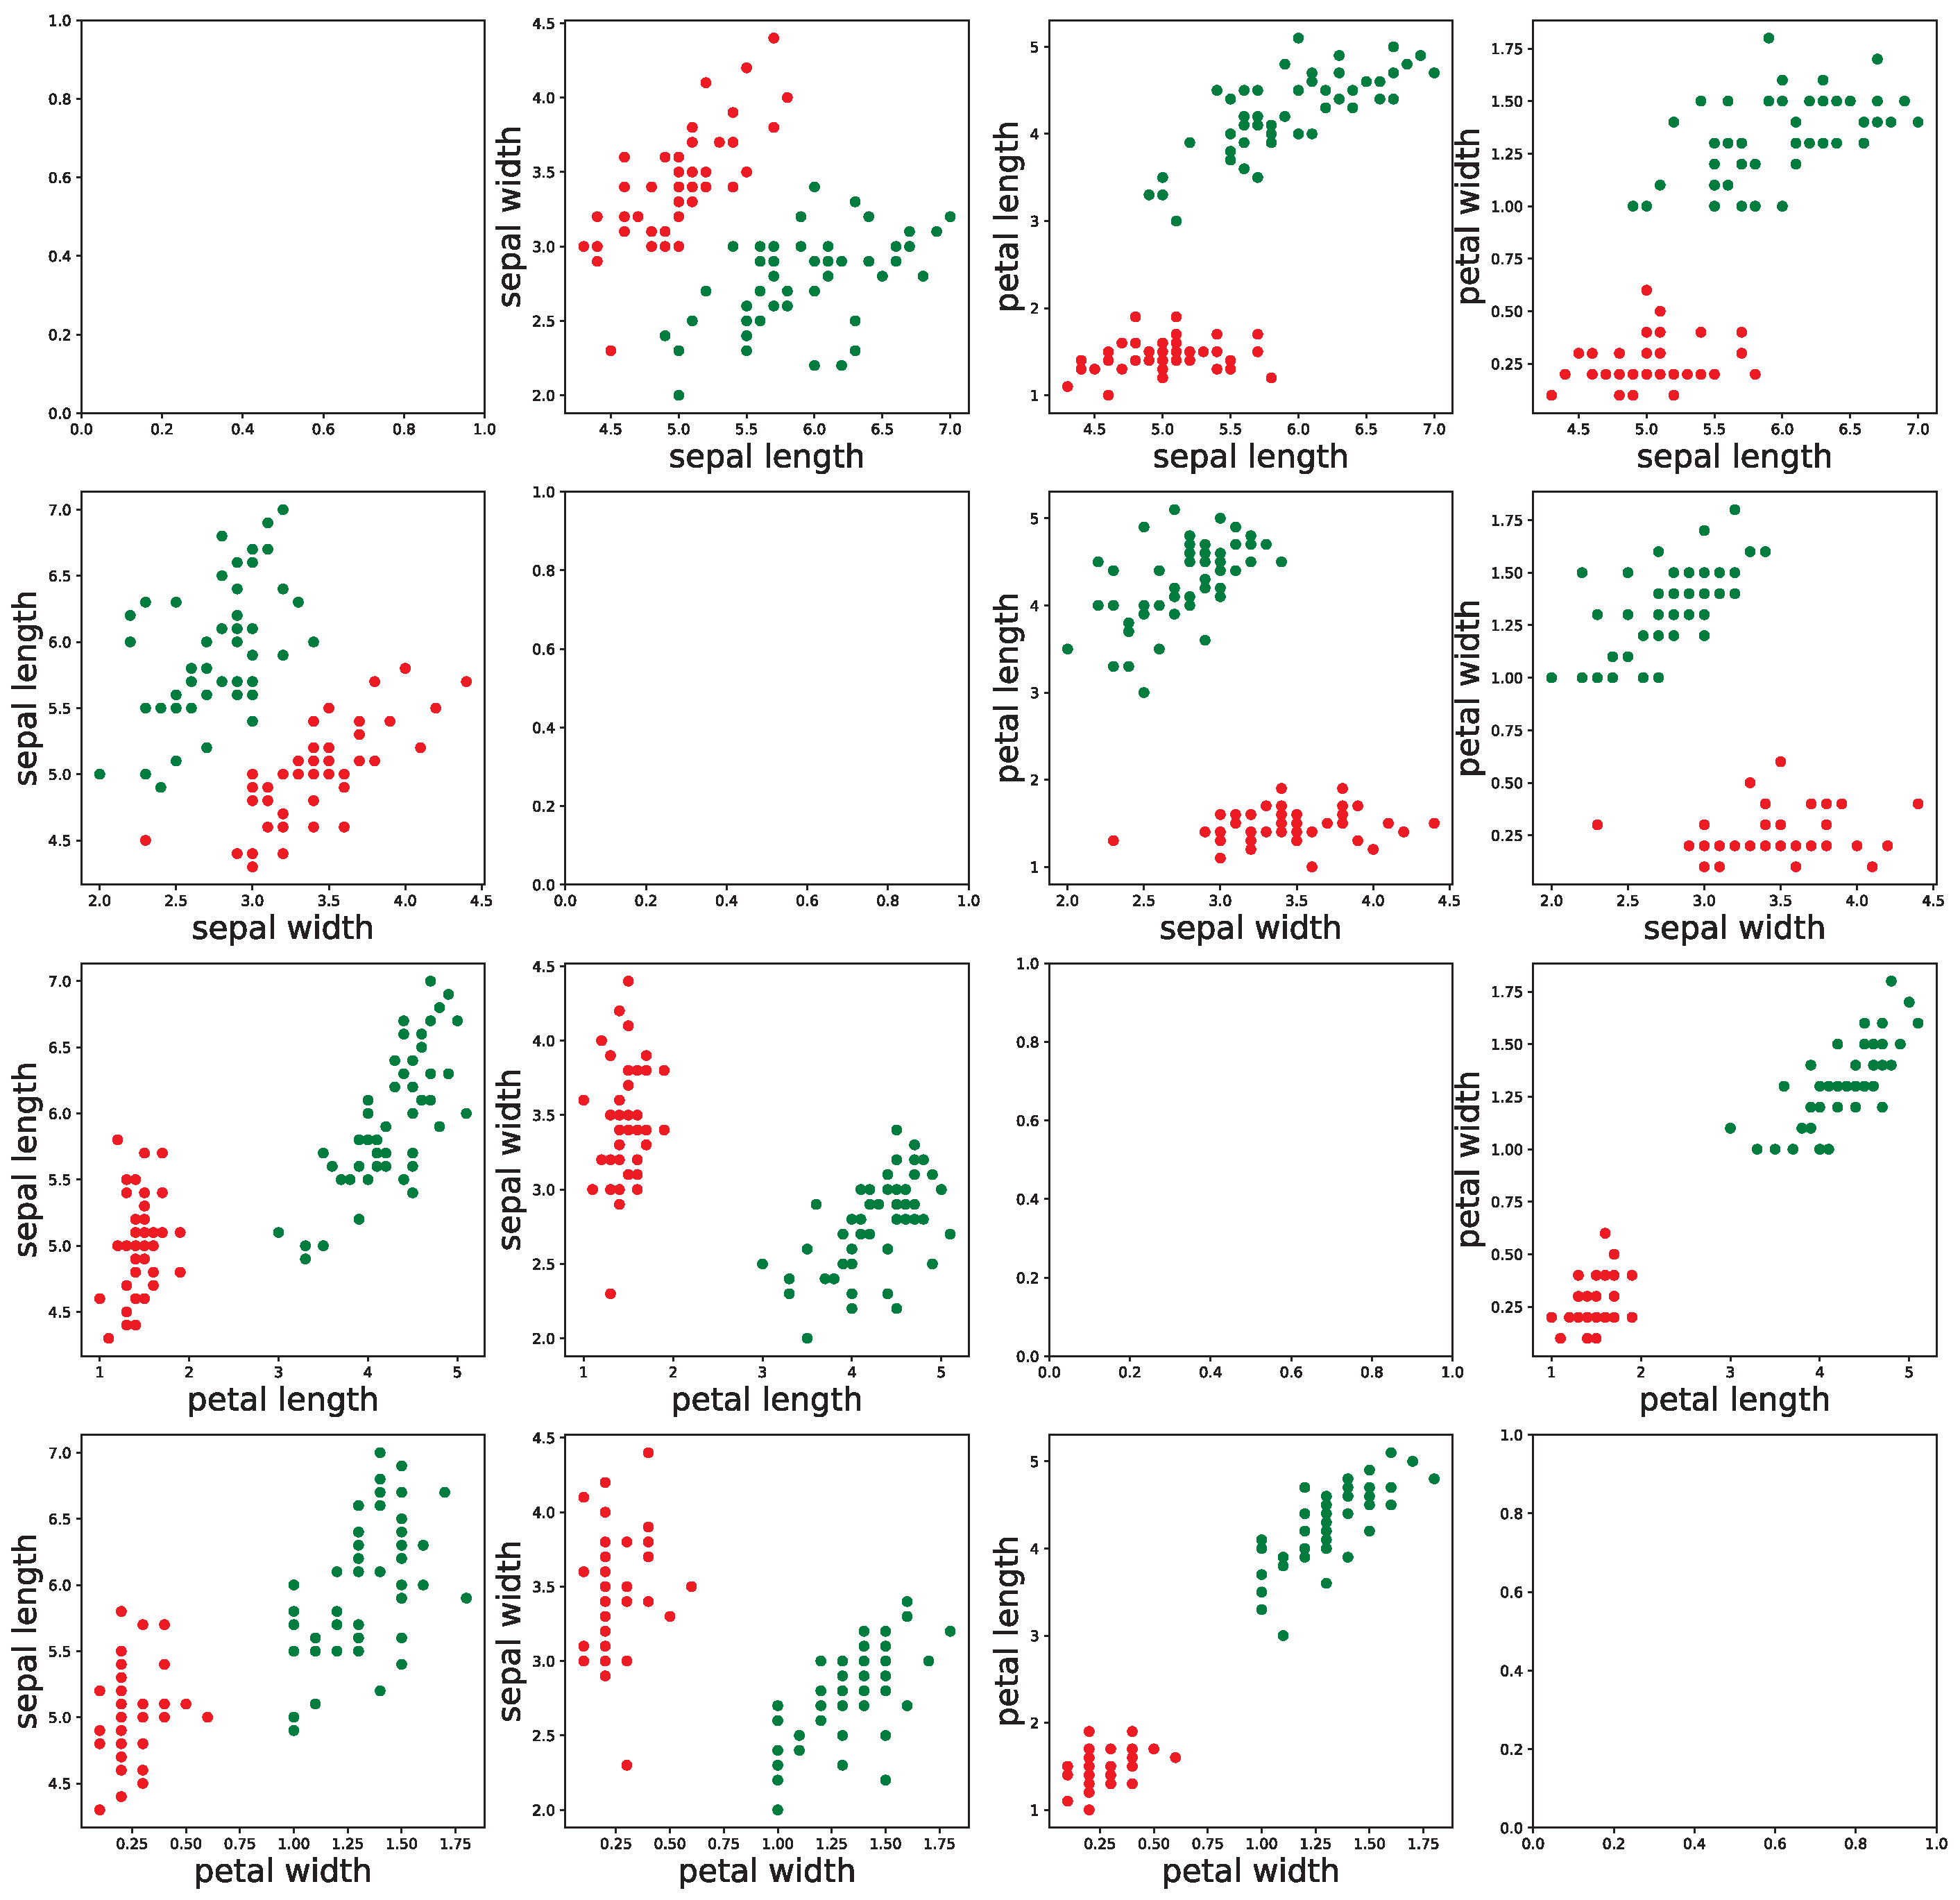
\includegraphics[width=0.8\textwidth]{5.1_figures/irisdataset_figure.eps}
%\caption{Visualization of iris dataset}
%\end{figure*}

%As seen in the images above, the red dots indicate samples with the label ``0'', while the green dots represent samples with the label ``1''.

\subsubsection{编码器与 Ansatz}
接下来，计算构建编码器所需的参数。执行以下命令。

\begin{lstlisting}
alpha = x[:, :3] * x[:, 1:]
x = np.append(x, alpha, axis=1)
\end{lstlisting}

构造特征是数据预处理中常用的技术。因此，此时每个样本具有 7 个特征：前四个特征值为原始特征值，后三个特征值由上述预处理计算得到。具体计算公式如下：

\begin{eqnarray}\label{5.1dataprocessing}
    X_{i+4}^{j} = X_{i}^{j} * X_{i+1}^{j},
\end{eqnarray}
其中 $i = 0, 1, 2$，$j = 1, 2, \cdots, 100$。

最后，通过运行下面的命令，将当前数据集划分为训练集和测试集。

\begin{lstlisting}
from sklearn.model_selection import train_test_split

x_train, x_test, y_train, y_test = train_test_split(x, y, test_size=0.2, random_state=0, shuffle=True)
\end{lstlisting}

此时训练集中有 80 个样本，测试集中有 20 个样本，每个样本都有 7 个特征。

接下来，需要在 MindSpore Quantum 中构建编码器，将经典数据编码为量子态。

这里采用的编码方法是 IQP 编码（Instantaneous Quantum Polynomial encoding）。一般而言，编码器的构建方式并非固定不变；可以根据当前问题的需求使用多种编码技术，有时还可以修改编码器以提升性能。

编码器中参数 $\alpha_0$, $\alpha_1$, $\cdots$,$\alpha_6$ 的取值由式~\eqref{5.1dataprocessing} 数据处理中得到的 7 个特征值代入。

现在，可以通过以下代码在 \MindQuantum\ 中构建编码器量子线路（见图~\ref{5.1encoder-circuit}）。

\begin{lstlisting}
from mindquantum import *

encoder = Circuit()

encoder += UN(H, 4)
for i in range(4):
    encoder += RZ(f'alpha{i}').on(i)
for j in range(3):
    encoder += X.on(j+1, j)
    encoder += RZ(f'alpha{j+4}').on(j+1)
    encoder += X.on(j+1, j)

encoder = encoder.no_grad()
encoder.svg()
\end{lstlisting}

\begin{figure}[H]
    \centering
    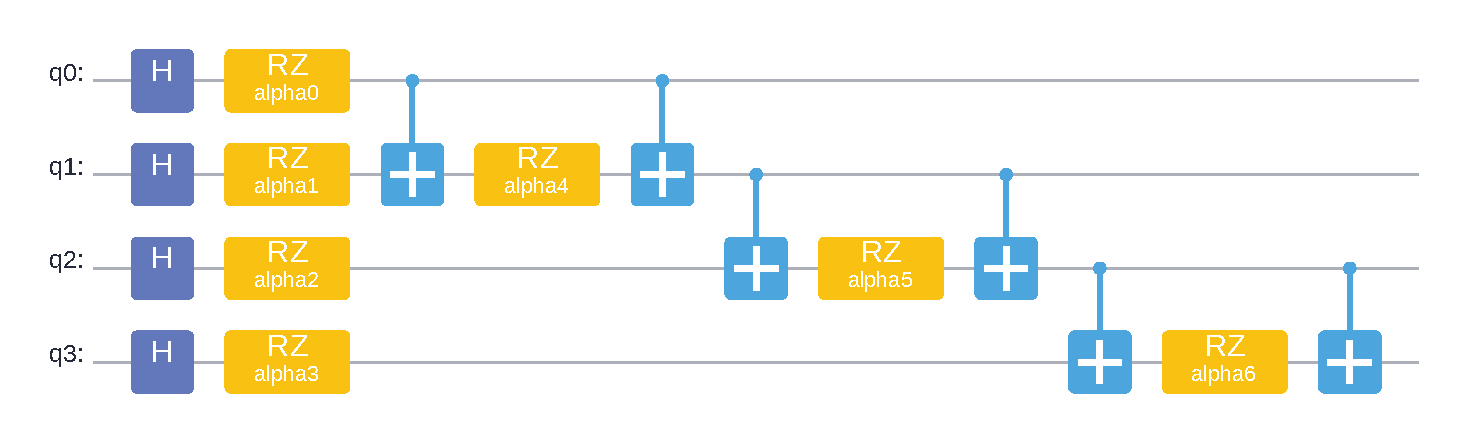
\includegraphics[width=0.49\textwidth]{5.1_figures/encoder-circuit.eps}
    \caption{IQP 编码器}
    \label{5.1encoder-circuit}
\end{figure}

从编码器线路可以看出，该量子线路由 17 个量子门组成，其中 7 个为参数化量子门，参数分别为 $\alpha_0$, $\alpha_1$, $\cdots$,$\alpha_6$。编码器线路调控的量子比特数量为 4。

此外，还需要在 MindSpore Quantum 中构建 ansatz。

与编码器类似，ansatz 的构建策略也很灵活，可以用于考察不同策略的有效性。

在本例中，我们使用 \HardwareEfficientAnsatz。通过以下代码得到的量子线路如图~\ref{5.1ansatz-circuit} 所示。

\begin{lstlisting}
ansatz = HardwareEfficientAnsatz(4, single_rot_gate_seq=[RY], entangle_gate=X, depth=3).circuit
ansatz.svg()
\end{lstlisting}

\begin{figure}[H]
    \centering
    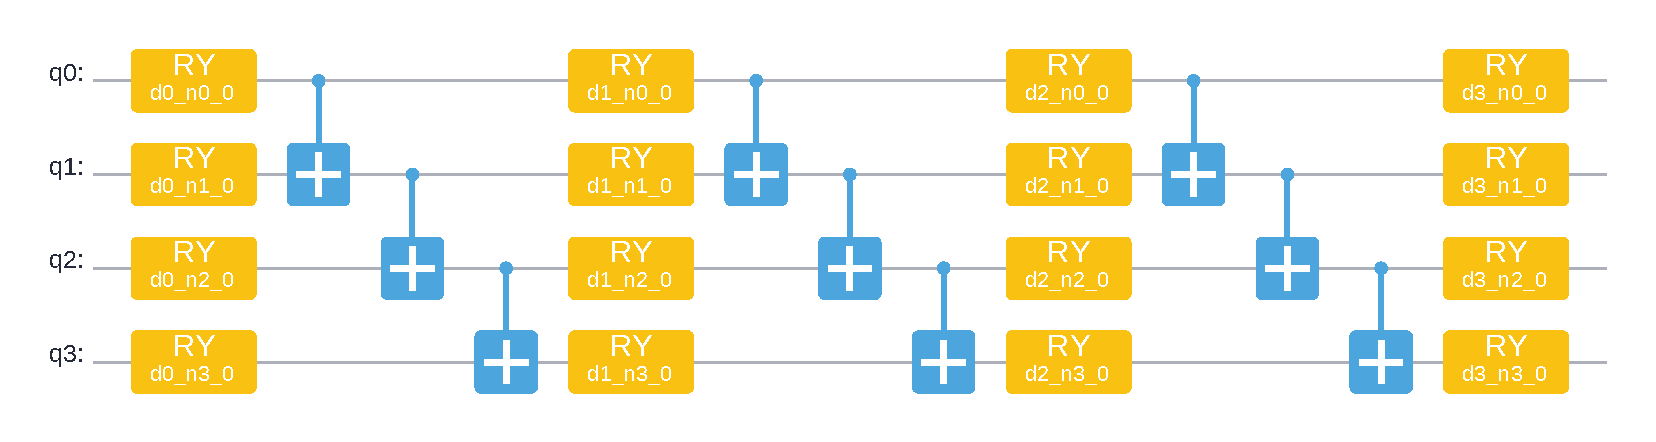
\includegraphics[width=0.49\textwidth]{5.1_figures/ansatz-circuit.eps}
    \caption{硬件高效 Ansatz}
    \label{5.1ansatz-circuit}
\end{figure}

从 ansatz 线路可以看出，该量子线路由 25 个量子门组成，其中 16 个为参数化量子门，参数分别为 $d0\_n0\_0$, $d0\_n1\_0$, $d0\_n2\_0$, $\cdots$。ansatz 线路调控的量子比特数量为 4。

在这种情况下，可以通过以下代码将编码器和 ansatz 组合成完整量子线路（见图~\ref{5.1total-circuit}）。

\begin{lstlisting}
circuit = encoder.as_encoder() + ansatz.as_ansatz()
circuit.svg()
\end{lstlisting}

\begin{figure}[H]
    \centering
    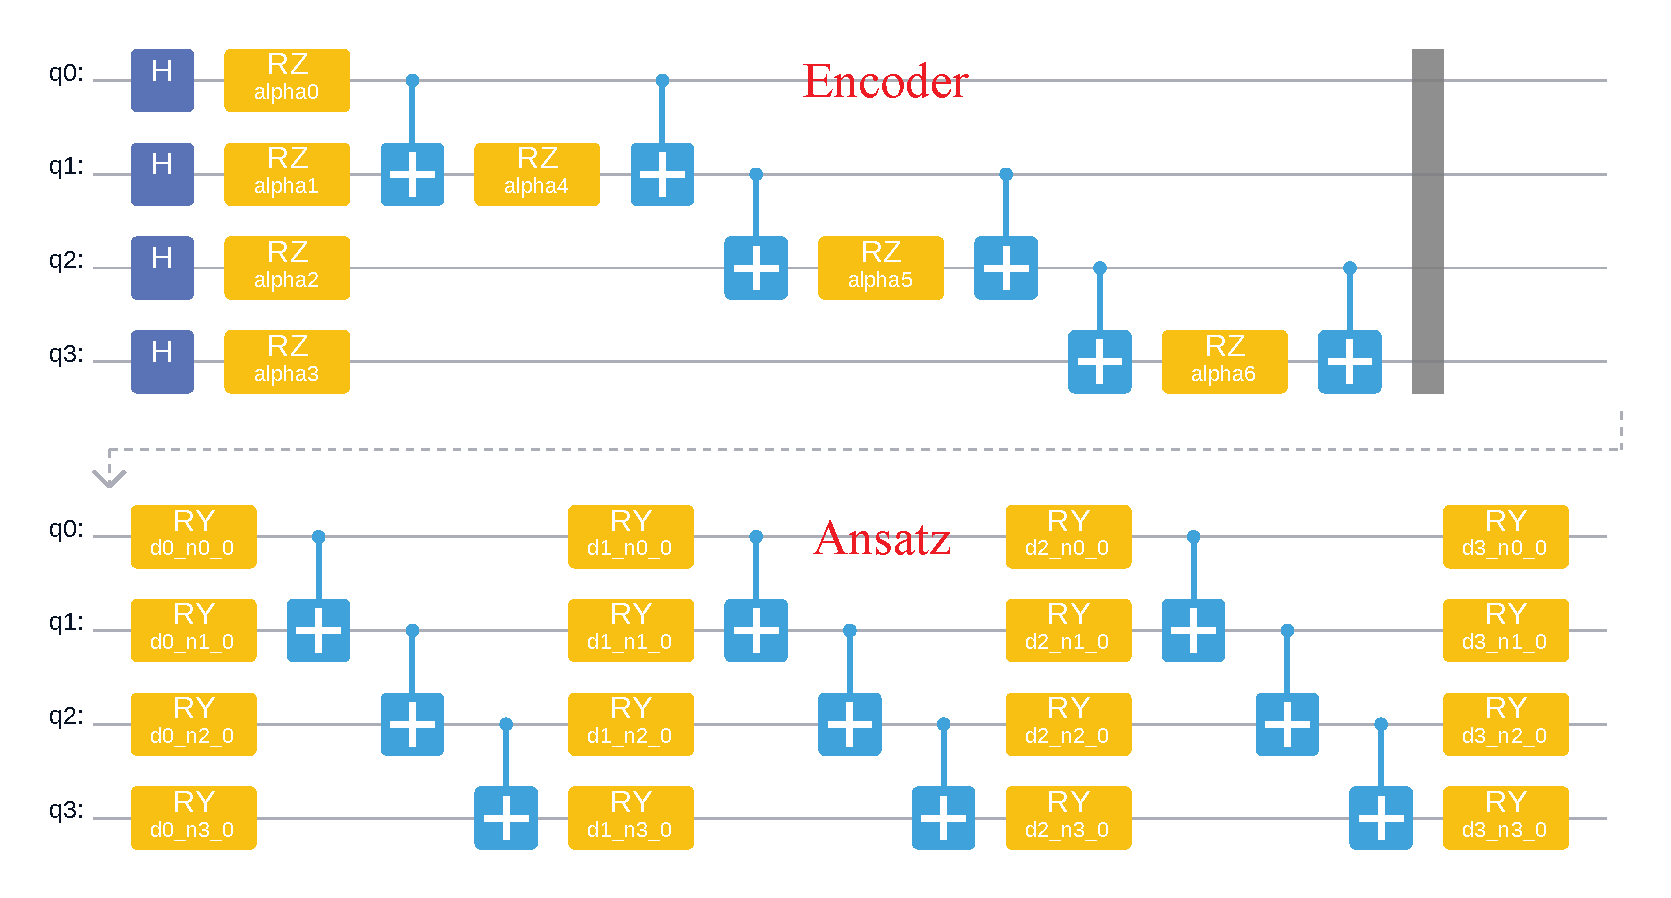
\includegraphics[width=0.49\textwidth]{5.1_figures/total-circuit.eps}
    \caption{完整量子线路}
    \label{5.1total-circuit}
\end{figure}

\subsubsection{哈密顿量}
我们分别在第二个和第三个量子比特上执行 Pauli $Z$ 算符测量，以创建对应的哈密顿量。执行以下代码。

\begin{lstlisting}
hams = [Hamiltonian(QubitOperator(f'Z{i}')) for i in [2, 3]]
for h in hams:
    print(h)
\end{lstlisting}

\begin{lstlisting}
1 [Z2]
1 [Z3]
\end{lstlisting}

从上述打印结果可以看出，此时构建了两个哈密顿量，分别是在第二个和第三个量子比特上作用 Pauli $Z$ 算符，并将系数设为 1。通过 Pauli $Z$ 算符测量，我们将得到两个哈密顿量测量值。

如果第一个测量值较大，则样本会被分类为标签为 ``0'' 的类别。类似地，如果第二个测量值较大，则样本会被分类为标签为 ``1'' 的类别。通过训练量子神经网络，我们期望训练样本中标签为 ``0'' 的样本具有更大的第一个测量值，标签为 ``1'' 的样本具有更大的第二个测量值。最后，将训练好的模型用于预测新样本的类别。

\subsubsection{训练}
通过以下命令构建量子神经网络。

\begin{lstlisting}
import mindspore as ms
from mindquantum.framework import MQLayer
from mindquantum.simulator import Simulator

ms.set_context(mode=ms.PYNATIVE_MODE, device_target="CPU")
ms.set_seed(1)
sim = Simulator('mqvector', circuit.n_qubits)
grad_ops = sim.get_expectation_with_grad(hams,
                                         circuit,
                                         parallel_worker=5)
QuantumNet = MQLayer(grad_ops)
QuantumNet
\end{lstlisting}

\begin{lstlisting}
MQLayer<
  (evolution): MQOps<4 qubits mqvector VQA Operator>
  >
\end{lstlisting}

从上述打印结果可以看出，我们已经成功构建了一个量子机器学习层，它可以与 MindSpore 中的其他算子无缝组成更大的机器学习网络。

接下来，需要定义损失函数并设置待优化参数。随后，将构建好的量子机器学习层与 MindSpore 算子组合成更大的机器学习网络。最后，对模型进行训练。%Follow the command below.

\begin{lstlisting}
from mindspore import LossMonitor, Model
from mindspore.nn import SoftmaxCrossEntropyWithLogits, Adam, Accuracy
from mindspore.dataset import NumpySlicesDataset
from mindspore.train import Callback

loss = SoftmaxCrossEntropyWithLogits(sparse=True, reduction='mean')
opti = Adam(QuantumNet.trainable_params(), learning_rate=0.1)

model = Model(QuantumNet, loss, opti, metrics={'Acc': Accuracy()})

train_loader = NumpySlicesDataset({'features': x_train, 'labels': y_train}, shuffle=False).batch(5)
test_loader = NumpySlicesDataset({'features': x_test, 'labels': y_test}).batch(5)

class StepAcc(ms.Callback):
    def __init__(self, model, test_loader):
        self.model = model
        self.test_loader = test_loader
        self.acc = []

    def step_end(self, run_context):
        self.acc.append(self.model.eval(self.test_loader, dataset_sink_mode=False)['Acc'])

monitor = LossMonitor(16)

acc = StepAcc(model, test_loader)

model.train(20, train_loader, callbacks=[monitor, acc], dataset_sink_mode=False)
\end{lstlisting}

\begin{lstlisting}
epoch: 1 step: 16, loss is 0.6140301823616028
epoch: 2 step: 16, loss is 0.48262983560562134
epoch: 3 step: 16, loss is 0.43457236886024475
epoch: 4 step: 16, loss is 0.4101267457008362
epoch: 5 step: 16, loss is 0.4027639925479889
epoch: 6 step: 16, loss is 0.39859312772750854
epoch: 7 step: 16, loss is 0.39496558904647827
epoch: 8 step: 16, loss is 0.3970319926738739
epoch: 9 step: 16, loss is 0.3954522907733917
epoch: 10 step: 16, loss is 0.39520972967147827
epoch: 11 step: 16, loss is 0.3955090641975403
epoch: 12 step: 16, loss is 0.3953099250793457
epoch: 13 step: 16, loss is 0.39525243639945984
epoch: 14 step: 16, loss is 0.3952508568763733
epoch: 15 step: 16, loss is 0.39521533250808716
epoch: 16 step: 16, loss is 0.39519912004470825
epoch: 17 step: 16, loss is 0.39518338441848755
epoch: 18 step: 16, loss is 0.395169198513031
epoch: 19 step: 16, loss is 0.39515653252601624
epoch: 20 step: 16, loss is 0.3951443135738373
\end{lstlisting}

训练过程中损失值持续下降，并在约 20 次迭代后趋于稳定，最终收敛在约 0.395。

根据上述收敛情况，可以展示训练过程中模型预测准确率的变化。%Run the following code.

\begin{lstlisting}
plt.plot(acc.acc)
plt.title('Statistics of accuracy', fontsize=20)
plt.xlabel('Steps', fontsize=20)
plt.ylabel('Accuracy', fontsize=20)

plt.show()
\end{lstlisting}

\begin{figure}[H]
    \centering
    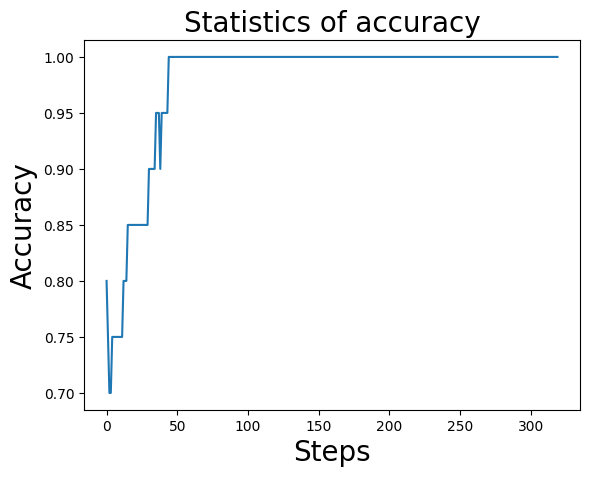
\includegraphics[width=0.4\textwidth]{5.1_figures/Statistics_of_accuracy.png}
    \caption{准确率统计}
    \label{5.1Statistics_of_accuracy}
\end{figure}

从图~\ref{5.1Statistics_of_accuracy} 可以看出，预测准确率在约 50 步后收敛到 1.00。

\subsubsection{预测}
最后，将训练好的模型应用到测试集上。
\begin{lstlisting}
from mindspore import ops

predict = np.argmax(ops.Softmax()(model.predict(ms.Tensor(x_test))), axis=1)
correct = model.eval(test_loader, dataset_sink_mode=False)

print("Predicted classification result:", predict)
print("Actual classification result:", y_test)

print(correct)
\end{lstlisting}

\begin{lstlisting}
Predicted classification result: [0 1 0 1 1 1 0 1 1 1 1 1 1 0 0 0 0 0 0 0]
Actual classification result: [0 1 0 1 1 1 0 1 1 1 1 1 1 0 0 0 0 0 0 0]
{'Acc': 1.0}
\end{lstlisting}

从上述打印结果可以看出，模型预测准确率达到 $100\%$，这意味着预测分类结果与实际分类结果完全一致。


\subsection{量子近似优化算法}


%To run this example in the browser through MindQuantum, follow the link:

%\href{https://blog.csdn.net/fisherish/article/details/105115272}{https://blog.csdn.net/fisherish/article/details/105115272}
%\cite{PhysRevLett.131.030402}
查看本节演示代码：\democode{05}{5.2_Quantum_Approximate_Optimization_Algorithm} \ \democodegithub{05}{5.2_Quantum_Approximate_Optimization_Algorithm}

\subsubsection{背景}

本节介绍量子近似优化算法（Quantum Approximate Optimization Algorithm, QAOA），并展示如何使用 \MindQuantum\ 实现该算法。此外，我们将在 D 节探索高级应用，在那里会应用 STA 技术实现收敛性更好的 ansatz DC-QAOA \cite{PhysRevResearch.4.013141}。


QAOA 是一种强大的量子算法，旨在利用量子计算机能力处理组合优化问题。该算法最早由 Farhi 等人在 2014 年提出 \cite{farhi2014quantum}；此后，人们发展出大量变体，用于克服原始算法的局限。

受量子绝热算法 Trotter 化版本的启发，QAOA 被归类为变分量子算法。传统 QAOA 由两个主要部分组成：量子部分涉及一个参数化线路 ansatz，经典部分负责优化这些参数。为了有效使用 QAOA 算法，我们将问题定义为寻找问题哈密顿量的基态。ansatz 由两个基本构件构成，即混合层和问题层：

\begin{equation}
    U(\gamma, \beta) = \prod_{l=1}^p e^{-i\beta_l \hat{H}_{m}}e^{-i\gamma_l\hat{H}{{p}}},
\end{equation}
其中，$\hat{H}_{{m}} = \sum_i \hat{\sigma}^x_i$ 表示混合哈密顿量，$\hat{\sigma}^x$ 对应 Pauli $x$ 算符；另一方面，$\hat{H}_{{p}}$ 表示问题哈密顿量。

量子态从 $\hat{H}_{\text{mixer}}$ 的基态开始，即 $|\psi_0\rangle=|+\rangle^{\otimes n}$。随后，QAOA ansatz 的量子态表示为：
\begin{equation}
    |\psi_p(\gamma, \beta)\rangle = e^{-i\beta_p\hat{H}_m}e^{-i\gamma_p\hat{H}_p}\cdots e^{-i\beta_1\hat{H}_{m}}e^{-i\gamma_1\hat{H}_{p}}|\psi_0\rangle.
\end{equation}
为了确定代价函数或目标函数，需要计算问题哈密顿量 $\hat{H}_{\text{prob}}$ 在 ansatz 态 $|\psi_p(\gamma, \beta)\rangle$ 上的期望值。这涉及在计算基下对最终态进行重复测量：
\begin{equation}
    F_p(\gamma, \beta) =\langle\psi_p(\gamma, \beta)|\hat{H}_{p} |\psi_p(\gamma,\beta)\rangle.
\end{equation}
QAOA 的主要目标是找到使期望值 $F_p(\gamma, \beta)$ 最小的最优参数 $(\gamma^*, \beta^*)$。实现这一目标需要使用经典优化算法迭代更新参数 $\gamma$ 和 $\beta$：
\begin{equation}
    (\gamma^*, \beta^*) = \text{arg}\min_{\gamma, \beta} F_p(\gamma, \beta).
\end{equation}

通过寻找这些最优参数，QAOA 使量子计算机能够高效应对复杂优化挑战，并为多种实际应用提供了有前景的途径。




\subsubsection{实现}

在本教程中，我们使用 QAOA 算法处理最大割问题，这是图论中的一个 NP 完全问题。如图 \ref{5.1_QAOA} 所示，该问题需要将图的顶点划分为两部分，并使被切割的边数量最大化。但当图中顶点数量增加时，很难找到有效的经典算法来求解最大割问题，因为这类 NP 完全问题很可能不存在多项式时间算法。

\begin{figure}[H]
    \centering
    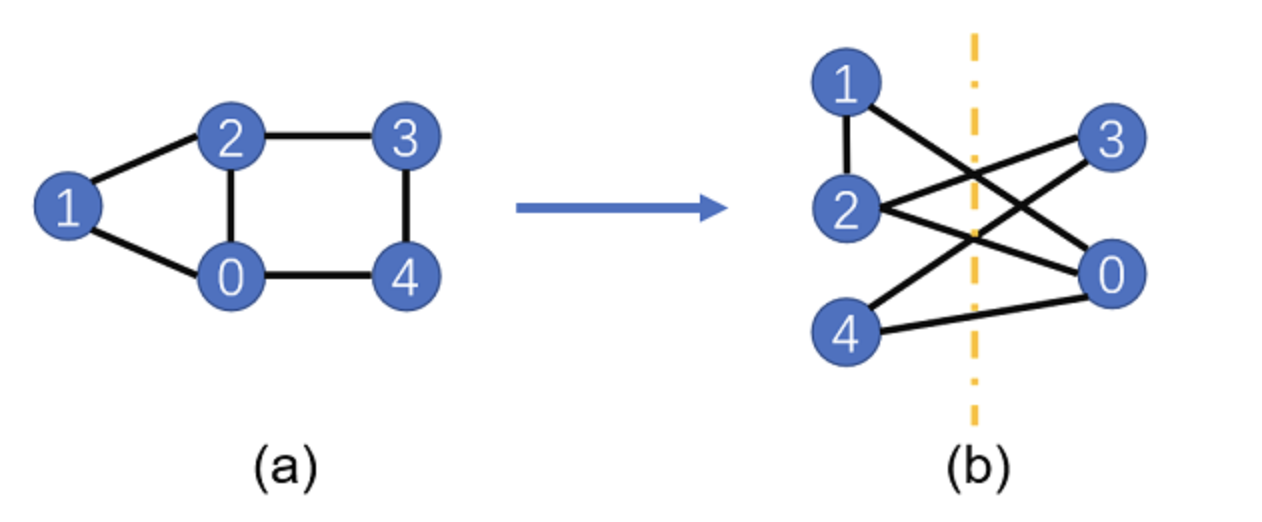
\includegraphics[width=0.49\textwidth]{5.2_figures/5.2_QAOA}
    \caption{最大割图}
    \label{5.1_QAOA}
\end{figure}

首先使用 \textit{NetworkX} \cite{SciPyProceedings_11} 生成一个由五个顶点和六条边组成的图结构。
\begin{lstlisting}
g = nx.Graph()
nx.add_path(g, [0,1])
nx.add_path(g, [1,2])
nx.add_path(g, [2,3])
nx.add_path(g, [3,4])
nx.add_path(g, [0,4])
nx.add_path(g, [0,2])
nx.draw(g,with_labels=True, font_weight='bold')
\end{lstlisting}

对于 QAOA 算法，首先需要将最大割问题转换为哈密顿量，其基态能量对应问题的解。最大割问题的问题哈密顿量可以构造为
\begin{equation}
    \hat{H} = \sum_{(i,j)\in C}(\hat{Z}_i\hat{Z}_j-1)/2,
\end{equation}
其中 $C$ 是所有边的集合。在下面的函数 \code{build\_ham} 中，可以通过输入图来构造对应哈密顿量。
\begin{lstlisting}
def build_ham(g):
    hc = QubitOperator()
    for i in g.edges:
        hc += QubitOperator(f'Z{i[0]} Z{i[1]}')
    return hc
\end{lstlisting}
接下来构造 QAOA ansatz，其中函数 \code{build\_hc} 和 \code{build\_hb} 分别根据问题哈密顿量和混合哈密顿量构造量子线路。通过向函数 \code{build\_ansatz} 输入图，可以直接构建 ansatz。

\begin{lstlisting}
def build_hc(g,para):
    hc = Circuit()
    for i in g.edges:
        hc += Rzz(para).on(i)
    return hc
def build_hb(g, para):
    hc = Circuit()
    for i in g.nodes:
        hc += RX(para).on(i)
    return hc
def build_ansatz(g, p):
    c = Circuit()
    for i in range(p):
        c += build_hc(g,f'g{i}')
        c += build_hb(g,f'b{i}')
    return c
\end{lstlisting}

在本例中选择 $p=4$，表示使用四层 QAOA 量子线路。\code{init\_state\_circ} 是用于将初态制备为均匀叠加态的量子线路。
\begin{lstlisting}
p = 4
ham = Hamiltonian(build_ham(g))
ansatz = build_ansatz(g, p)
init_state_circ = UN(H, g.nodes)
\end{lstlisting}

QAOA 的目标是找到最优参数，使代价函数或哈密顿量期望值 $\mathcal{E}=\langle \psi(\gamma, \beta)|\hat{H}|\psi(\gamma, \beta)\rangle$ 最小。
该问题不需要编码层量子线路，因此我们使用 \MQAnsatzOnlyLayer\ 作为待训练的量子神经网络，并使用 Adam 作为优化器。
\begin{lstlisting}
import mindspore as ms
ms.set_context(mode=ms.PYNATIVE_MODE, device_target="CPU")

total_circuit = init_state_circ + ansatz
sim = Simulator('mqvector', total_circuit.n_qubits)
grad_ops = sim.get_expectation_with_grad(ham, total_circuit)
net = MQAnsatzOnlyLayer(grad_ops)
opti = nn.Adam(net.trainable_params(), learning_rate=0.05)
train_net = nn.TrainOneStepCell(net, opti)

for i in range(600):
    if i%10 == 0:
        print("train step:", i, ", cut:", (len(g.edges)-train_net())/2)
\end{lstlisting}
\begin{lstlisting}
train step: 0 ,   cut: [3.0001478]
train step: 10 ,  cut: [4.1718774]
train step: 20 ,  cut: [4.6871986]
train step: 30 ,  cut: [4.7258005]
train step: 40 ,  cut: [4.804503]
train step: 50 ,  cut: [4.8477592]
train step: 60 ,  cut: [4.8705964]
train step: 70 ,  cut: [4.9060946]
train step: 80 ,  cut: [4.933446]
train step: 90 ,  cut: [4.9356637]
train step: 100 , cut: [4.938308]
train step: 110 , cut: [4.9390197]
train step: 120 , cut: [4.939068]
train step: 130 , cut: [4.9392157]
train step: 140 , cut: [4.939249]
train step: 150 , cut: [4.939247]
train step: 160 , cut: [4.939255]
train step: 170 , cut: [4.939257]
train step: 180 , cut: [4.939257]
train step: 190 , cut: [4.939257]
\end{lstlisting}

根据上述训练结果可以发现，该问题哈密顿量基态能量对应的割边数量接近 5。

在 \MindQuantum\ 中，可以直接导入 \MaxCutAnsatz\ 函数来构建最大割问题的 ansatz。
\begin{lstlisting}
import numpy as np
from mindquantum.algorithm.nisq import MaxCutAnsatz
graph = [(0, 1), (1, 2), (0, 2)]
p = 1 # 层数
maxcut = MaxCutAnsatz(graph, p)
maxcut.circuit.svg()
\end{lstlisting}
\begin{figure}[H]
    \centering
    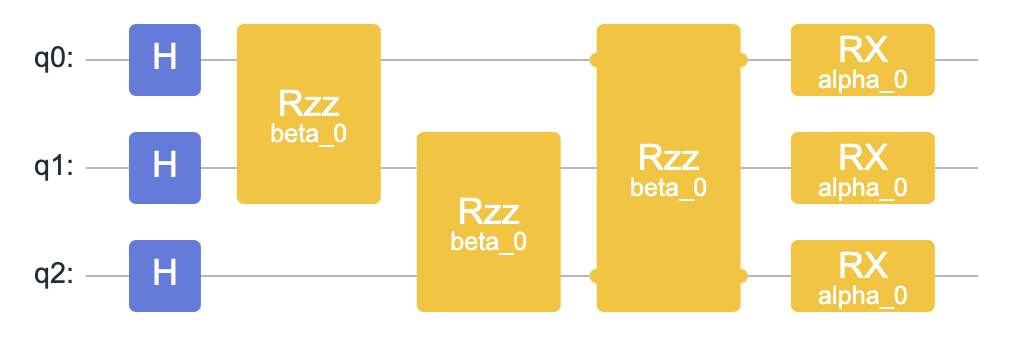
\includegraphics[width=0.49\textwidth]{5.2_figures/5.2_QAOA_ansatze}
    \caption{最大割问题 Ansatz}
    \label{5.1_QAOA_ansatz}
\end{figure}
同时，也可以获得哈密顿量：
\begin{lstlisting}
print(maxcut.hamiltonian)
\end{lstlisting}
\begin{lstlisting}
3/2 [] +
-1/2 [Z0 Z1] +
-1/2 [Z1 Z2] +
-1/2 [Z0 Z2]
\end{lstlisting}
最大割问题的切割方案以及该方案中的割边数量，可以通过函数 $get\_partition$ 和 $get\_cut\_value$ 获得。切割方案是由两个列表组成的列表数组，每个列表数组都包含被切分到对应部分的节点。
\begin{lstlisting}
partitions = maxcut.get_partition(5, np.array([4, 1]))
for i in partitions:
    print(f'partition: left: {i[0]}, right: {i[1]}, cut value: {maxcut.get_cut_value(i)}')
\end{lstlisting}
\begin{lstlisting}
partition: left: [0, 2],   right: [1], cut value: 2
partition: left: [1, 2],   right: [0], cut value: 2
partition: left: [1],   right: [0, 2], cut value: 2
partition: left: [0, 1, 2], right: [], cut value: 0
partition: left: [], right: [0, 1, 2], cut value: 0
\end{lstlisting}











\subsection{变分量子本征求解器}
%Pauli encoding
%Ansatz and initial trial function
%Measurement
%variational method and optimization
%classical optimization methods
% an example for simulating the ground energy of a Molecule

查看本节演示代码：\democode{05}{5.3_Variational_Quantum_Eigensolver} \ \democodegithub{05}{5.3_Variational_Quantum_Eigensolver}

\subsubsection{背景}

在量子计算中，变分量子本征求解器（Variational Quantum Eigensolver, VQE）是在近期量子计算机上求解本征问题的代表性算法。该算法最初由 Peruzzo 等人提出，其理论框架由 McClean 等人扩展并形式化 \cite{Peruzzo2014Peruzzo2014}。
VQE 被广泛用于计算分子和材料的能量性质，例如电子结构研究，这是量子化学和凝聚态物理中的关键应用。
传统计算化学为小规模系统提供了高效近似此类性质的方法，但随着系统规模增大，极高精度计算会变得难以处理且代价高昂。此外，电子之间的相互作用在形式上要求计算量随系统规模指数增长，使得精确量子化学方法通常无法通过传统计算有效处理。
这一瓶颈正是研究 VQE 等方法的动机，人们期待这些方法有朝一日能够在此类问题上超越传统计算范式。

从最一般的描述来看，VQE 旨在通过 Ritz 变分原理近似给定哈密顿量 $\hat{H}$ 的基态能量 $E_0$（指定 Hilbert 空间中的最小本征值）及其对应基态 $|E_0\rangle$。
给定复厄米矩阵 $M$ 和非零向量 $x$，Rayleigh 商定义为：
\begin{equation}
    R(M,x)=\frac{x^*Mx}{x^*x}.
\end{equation}
且 $R(M,x)$ 总满足 $E_0\leq R(M,x)\leq E_N$（分别为最小和最大本征值）。

也就是说，给定一个感兴趣的哈密顿量 $\hat{H}$ 和预设波函数 $|\psi\rangle$，$\hat{H}$ 的基态能量 $E_{0}$ 总满足
\begin{equation}
    E_0 \leq \frac{\langle \psi |\hat{H}| \psi \rangle}{\langle \psi |\psi\rangle}.
\end{equation}
因此，VQE 的主要目标是找到一个合适的 $|\psi^*\rangle$，使 $\hat{H}$ 的期望值最小。若基态能量非简并，则有 $|E_0\rangle = |\psi^*\rangle$ 且 $E_0 = \langle \psi^* |\hat{H}| \psi^* \rangle$。（如果基态能量简并，则 $|\psi^*\rangle$ 通常位于所有基态张成的空间中。）

然而，由于直接寻找 $|\psi^*\rangle$ 是一个难以处理的问题，VQE 首先定义所谓 ansatz 波函数 $|\psi(\vec{\theta})\rangle$。该波函数可以在量子设备上实现为一系列量子门，其行为由参数 $\vec{\theta}$ 描述。

VQE 的另一个特征是它是一种同时使用经典计算机和量子计算机的混合算法。
量子本征求解器旨在寻找给定哈密顿量 $\hat{H}$ 的本征值和本征态。
Ritz 变分原理告诉我们，对于给定 $\hat{H}$ 和任意态 $|\vec{\theta}\rangle$，
\begin{equation}
    \lambda_{\min}\leq \frac{\langle \vec{\theta} |\hat{H}| \vec{\theta}\rangle}{\langle \vec{\theta}|\vec{\theta}\rangle} \leq \lambda_{\max},
\end{equation}
其中 $\lambda_{\min, \max}$ 是 $\hat{H}$ 的最小（最大）本征值，并且在量子计算中有 $\langle \vec{\theta}|\vec{\theta}\rangle = 1, \forall \vec{\theta}$。
借助 Ritz 变分原理，VQE 将本征问题转换为迭代优化问题，其代价函数为 $\min_{\vec{\theta}}\hat{E}= \langle \vec{\theta} |\hat{H}| \vec{\theta}\rangle$。
如果 $\hat{H}$ 的基态非简并，通过经典优化器优化 $\vec{\theta}$ 的取值以最小化 $\hat{E}$，即可得到 $\hat{E}(\vec{\theta}^*)\approx E_{gs}$ 且 $|\langle \vec{\theta}^*|E_0\rangle| \approx 1$。

VQE 从一个初始化量子比特态开始。随后，对该态施加参数化量子线路，以建模电子波函数的物理性质和纠缠结构。

VQE 流程包括：
\begin{itemize}
    \item 哈密顿量构造与表示：从费米子空间到量子比特空间的变换、算符编码
    \item Ansatz 选择与态制备：硬件高效 ansatz、QubitUCCAnsatz、UCCAnsatz、Hartree-Fock 态
    \item 测量：期望值
    \item 参数优化：优化器、参数平移规则、有限差分、自动微分
          %\item Error mitigation
\end{itemize}

\subsubsection{实现}

在使用 VQE 研究任何物理模型或分子之前，考虑到当前主流量子平台以量子比特为基础，必须先将其转换为量子比特哈密顿量。
这里，我们展示 \MindQuantum\ 如何逐步模拟量子化学示例 LiH。
首先需要导入所需软件包。
\begin{lstlisting}
from openfermion.chem import MolecularData
from openfermionpyscf import run_pyscf
\end{lstlisting}
\code{openfermion} 和 \code{openfermionpyscf} 是开源软件包，可用于为给定化学分子构型构造对应哈密顿量。例如，可以按如下方式定义 LiH 分子几何结构：
\begin{lstlisting}
    dist=1.5
    geometry=[
    ["Li",[0.0,0.0,0.0*dist]],
    ["H",[0.0,0.0,1.0*dist]]
    ]
    basis="sto3g"
    spin = 0
    molecule = MolecularData(geometry,basis,multiplicity=2*spin+1)
    molecule = run_pyscf(molecule,run_scf=1,run_ccsd=1,run_fci=1)
\end{lstlisting}
基于 \code{molecule}，可以使用 \MindQuantum\ 中的函数获得对应量子比特哈密顿量表达式：
\begin{lstlisting}
    from mindquantum.algorithm.nisq import get_qubit_hamiltonian
    hamiltonian_QubitOP = get_qubit_hamiltonian(molecule)
\end{lstlisting}
至此，我们已经方便地完成了 LiH 哈密顿量表达式的构建。
VQE 的下一步是选择良好的波函数 ansatz。酉耦合簇单双激发（Unitary Coupled-Cluster Singles and Doubles, UCCSD）方法受量子化学中经典 CCSD 的启发。在 \MindQuantum\ 中，可以通过如下方式构建 LiH 的 UCCSD ansatz：
\begin{lstlisting}
    from mindquantum.algorithm.nisq import uccsd_singlet_generator, uccsd_singlet_get_packed_amplitudes
    ucc_fermion_ops = uccsd_singlet_generator(
    molecule.n_qubits, molecule.n_electrons, anti_hermitian=True)
    ucc_qubit_ops = Transform(ucc_fermion_ops).jordan_wigner()
    ansatz_circuit = TimeEvolution(ucc_qubit_ops.imag, 1.0).circuit
ansatz_parameter_names = ansatz_circuit.params_name
\end{lstlisting}
通常，对于该化学问题，VQE 的初态为 Hartree-Fock 态。我们施加 Pauli $X$ 门，以确保初态中 $|1\rangle$ 的数量等于分子中的电子数。
\begin{lstlisting}
    hartreefock_wfn_circuit = Circuit([X.on(i) for i in range(molecule.n_electrons)])
\end{lstlisting}
因此，用于求解 LiH 基态能量的 VQE 总量子线路为：
\begin{lstlisting}
    total_circuit = hartreefock_wfn_circuit + ansatz_circuit
\end{lstlisting}

在 VQE 中，通常选择梯度下降方法作为优化器，以获得能够输出最小期望值的最优参数。
在 \MindQuantum\ 中，可以方便地利用 MindSpore Quantum 获得梯度算符。
梯度算符是一个特殊函数：输入初始参数后，它可以输出对应梯度值。
在 \MindQuantum\ 中，VQE 的梯度算符可以通过如下方式获得：
\begin{lstlisting}
    grad_ops = Simulator('mqvector', total_circuit.n_qubits).get_expectation_with_grad(
    Hamiltonian(hamiltonian_QubitOp.real),
    total_circuit)
\end{lstlisting}
上述流程把费米子哈密顿量和 UCC ansatz 都转换到量子比特线路上，因此适合与真实量子芯片执行、线路编译以及通用模拟器保持一致。若研究目标是量子化学 VQE 的数值实验，且 ansatz 主要由 UCC 单、双激发构成，也可以使用第~\ref{sec:mqchem} 节介绍的 \texttt{mqchem} 后端。该后端直接在固定电子数 CI 子空间中保存波函数，并通过 \texttt{UCCExcitationGate} 与 \texttt{CIHamiltonian} 计算能量和梯度，从而避免把每个费米子激发先展开为 Pauli 演化线路。
通常，需要为线路提供合适的初始参数，以便更快收敛到最小值。对于 UCCSD ansatz，CCSD 值是一个很好的选择，可以通过如下方式获得：
\begin{lstlisting}
    init_amplitudes_ccsd = uccsd_singlet_get_packed_amplitudes(
    molecule_of.ccsd_single_amps, molecule_of.ccsd_double_amps, molecule_of.n_qubits, molecule_of.n_electrons)
init_amplitudes_ccsd = [init_amplitudes_ccsd[param_i] for param_i in ansatz_parameter_names]
\end{lstlisting}
至此，我们已经准备好了 VQE 所需的全部内容。
VQE 的最后一步是最小化代价函数以得到能量期望值，这可以使用 \textit{SciPy} 包完成。
\begin{lstlisting}
    from scipy.optimize import minimize

    def fun(theta, grad_ops, energy_list):
        energy, grad = grad_ops(theta)
        energy_list.append(energy)
        return np.squeeze(energy.real), np.squeeze(grad.real)

    energy_list = []
    res = minimize(fun, p0, args=(grad_ops, energy_list), method='bfgs', jac=True)
\end{lstlisting}
如果一切正常，将得到类似如下结果：
\begin{lstlisting}
    Step: 5,        energy: -7.878223282730547
    Step: 10,       energy: -7.880288481438961
    Step: 15,       energy: -7.882035668304055
    Step: 20,       energy: -7.882302370885741
    Step: 25,       energy: -7.882349803534313
    Step: 30,       energy: -7.882352702053751
    Step: 35,       energy: -7.8823527077335065
    Step: 40,       energy: -7.882352708347106
\end{lstlisting}
至此，我们已经使用 \MindQuantum\ 找到了基态能量的近似值。此外，我们还注意到一种新的量子本征求解器算法，即全量子本征求解器（Full Quantum Eigensolver, FQE）算法 \cite{wei2020full}。该算法不需要经典优化器，而是利用量子梯度下降直接在量子计算机上完成所有计算。


\subsection{DC-QAOA}


%To run this example, follow the link
查看本节演示代码：\demonotebook{05}{5.4_DC_QAOA} \ \demonotebookgithub{05}{5.4_DC_QAOA}

\subsubsection{背景}
在量子计算领域，研究人员持续寻求高效且鲁棒的方法来处理复杂问题。绝热量子计算（Adiabatic Quantum Computation, AQC）就是这样一种方法，其中量子系统从初始哈密顿量逐渐演化到编码目标解的最终哈密顿量。根据绝热定理，如果该演化足够缓慢，系统将在整个过程中保持在哈密顿量的基态：
\begin{equation}
    H(t) = (1-\lambda(t))H_{\text{initial}} + \lambda(t)H_{\text{final}},
\end{equation}
其中 \(\lambda(t) \in [0, 1]\)。然而，在实际场景中执行 AQC 会面临外部噪声、器件不完美以及需要长时间演化等挑战。为了克服这些限制并提升绝热演化效率，一个有前景的方案是量子近似优化算法（QAOA）。

QAOA 使用参数化量子线路制备试探态，以近似优化问题的解。通过优化 ansatz 参数，QAOA 寻找使目标函数最小的最优取值，而目标函数编码了问题的能量景观。这种方法能够缩短演化时间，并对噪声和不完美因素具有更强鲁棒性，因此在实际量子计算应用中可作为 AQC 的可行替代方案。

然而，QAOA 的硬件实现仍会受到噪声、退相干以及参数优化复杂性的挑战。为提升其性能和鲁棒性，数字化反绝热量子近似优化算法（Digitized Counterdiabatic Quantum Approximate Optimization Algorithm, DC-QAOA）引入了反绝热（counterdiabatic, CD）项：

\begin{equation}
    H_{\text{DC-QAOA}} = H_{\text{initial}}(\gamma) + H_{\text{final}}(\beta) + H_{\text{CD}}(\alpha),
\end{equation}

该方法结合了绝热量子计算（AQC）与 QAOA 的思想。与 QAOA 相比，它在每层中引入一个额外参数，从而在不牺牲精度的情况下得到更浅的量子线路：
\begin{equation}
    \label{eq:evo operator}
    U(\gamma, \beta) \to U(\gamma, \beta, \alpha), \quad F(\gamma, \beta) \to F(\gamma, \beta, \alpha),
\end{equation}
其中 \(\alpha\)、\(\beta\) 和 \(\gamma\) 表示数字化参数，\(F\) 为代价函数，\(U\) 为演化算符。

CD 项作为哈密顿量中的额外组成部分，基于演化哈密顿量的瞬时本征态和本征能量设计。它能够有效抑制误差并减少所需演化时间，从而提升量子计算的效率和可靠性。

为了推导反绝热项的精确形式，人们已经应用了多种技术，例如 Lewis-Riesenfeld 不变量和无跃迁量子驱动~\cite{PhysRevA.83.062116}。CD 项的实现会根据具体问题和量子系统动力学进行定制，并利用可用控制技术。当难以获得精确 CD 项时，可以采用一种近似 CD 驱动方法，即结合绝热规范势使用嵌套对易子方法~\cite{PhysRevResearch.4.013141}：

\begin{equation}
    A_{\lambda}^{(l)} = i \sum_{k=1}^{l} \alpha_{k}(t) [H_{a}, [H_{a}, \ldots, [H_{a}, \partial_{\lambda} H_{a}]]].
\end{equation}

DC-QAOA 有望用于求解广泛的优化问题，从组合优化到蛋白质折叠~\cite{PhysRevApplied.20.014024} 和金融投资组合优化~\cite{PhysRevResearch.4.043204}。随着量子计算技术持续发展，DC-QAOA 为利用反绝热项和参数空间数字化开拓量子优化新前沿提供了令人期待的途径。

\textbf{目标问题}
\begin{itemize}
    \item[1.] 学习如何寻找问题哈密顿量的基态
    \item[2.] 利用量子线路寻找优化参数
\end{itemize}
\textbf{所需 MindQuantum 功能}
\begin{itemize}
    \item[1.] 基于梯度的优化器
    \item[2.] 批量量子线路模拟器

\end{itemize}

\subsubsection{实现}
作为变分算法的一种成熟变体，该方法需要两个步骤：构建 ansatz 线路和执行优化。现在来看如何将 DC-QAOA 应用于 Ising 模型~\cite{PhysRevResearch.4.013141}。哈密顿量的一般形式由下式给出：

\begin{equation}
    H_{final} = H_{prob} = -J_{ij}\sum_{i=1}^{n-1}\sigma^z_i\sigma^z_{i+1}-h_{i}\sum_{i=1}^{n}{\sigma_i^z} + k_{i}\sum_{i=1}^{n}\sigma_{i}^{x}.
\end{equation}

初态选为 $H_{initial} = \sum_{i}\sigma_{i}^{x}$，它应当驱动不同态之间的跃迁，从而促进对解空间的探索。具体而言，我们选择纵场 Ising 模型（longitudinal field Ising model, LFIM）哈密顿量，其中 $J_{ij}=1,~h_{i}=1,~k_{i}=0$。
\begin{lstlisting}
# 生成作为 H_{mixer} 的 H_{initial}.
# n_qubits 是量子比特数量
def generate_h_mixer(n_qubits:int):
    h_mixer = QubitOperator()
    for i in range(n_qubits):
        h_mixer += QubitOperator(f'X{i}')
    return h_mixer

# 生成作为 H_{prob} 的 H_{final}.
def generate_h_prob(n_qubits:int, J:float, h:float):
    h_prob = QubitOperator()
    for i in range(n_qubits-1):
        h_prob += QubitOperator(f'Z{i} Z{i+1}', -J)
    for i in range(n_qubits):
        h_prob += QubitOperator(f'Z{i}', -h)
    return h_prob
\end{lstlisting}

在本例中，使用绝热规范势的嵌套对易子方法定义一个 CD 算符池~\cite{PhysRevResearch.6.013147}：
$$A = \{\sigma^{y},\sigma^{z}\sigma^{y}, \sigma^{y}\sigma^{z}, \sigma^{x}\sigma^{y}, \sigma^{y}\sigma^{x} \}.$$
这里给出一个 12 量子比特系统，并考虑 CD 项为 $A^{*} = \sum_{i=1}^{n}\sigma_{i}^{y}$。接下来构建 DC-QAOA 的 ansatz 层。
\begin{lstlisting}
def generate_h_cd(n_qubits:int):
    h_cd = QubitOperator()
    for i in range(n_qubits):
        h_cd += QubitOperator(f'Y{i}')
    return h_cd
\end{lstlisting}

\begin{lstlisting}
n_qubits = 12
J, h = 1, 1

h_prob = generate_h_prob(n_qubits, J, h)
h_mixer = generate_h_mixer(n_qubits)
h_cd = generate_h_cd(n_qubits)
\end{lstlisting}

为了制备 $H_{initial}$ 的本征态，我们首先构造 ${\rm prep\_circ}$，随后在其上施加演化算符。
\begin{lstlisting}
# 制备 $H_{mixer}$ 的本征态。
prep_circ = UN(H, n_qubits)
# 选择层数 p。
p = 1

ansatz_template =   u_p + u_m  + u_cd

ansatz = Circuit() + prep_circ

for i in range(p):
    ansatz += add_suffix(ansatz_template, str(i)) + BarrierGate()
\end{lstlisting}

只要设置好了 ansatz 线路，就可以改变层数或经典优化器类型，以寻找最优参数集合。我们定义代价函数为
\begin{equation}
    F(\alpha,~\beta,~\gamma) = \left<\psi_0\right|U^{\dagger}\ H_{prob} U\left|\psi_0\right>,
\end{equation}
其中 $U = \Pi_{i=0}^p U_{cd}(\alpha_i)U_m(\beta_i)U_p(\gamma_i)$，这正是式~\ref{eq:evo operator} 中的演化算符。
\begin{lstlisting}
def train(ham, ansatze, iteration):

    # 构建量子线路

    circ = ansatze
    sim = Simulator('mqvector', ansatze.n_qubits)

    grad_ops = sim.get_expectation_with_grad(ham, circ)
    net = MQAnsatzOnlyLayer(grad_ops)
    opti = nn.Adagrad(net.trainable_params(), learning_rate=0.05)
    train_net = nn.TrainOneStepCell(net, opti)

    result = []
    for i in range(iteration):
        train_net()
        result.append(np.array(train_net()[0]))
    pr = dict(zip(ansatze.params_name, net.weight.asnumpy()))

    return result
\end{lstlisting}

在本教程中，我们使用 Adam 优化器~\cite{PhysRevResearch.6.013147} 优化梯度，它能够给出足够好的结果。绘制平均能量图后可得到图~\ref{fig:dc}。其中，绿色虚线是 $H_{prob}$ 的精确本征值，蓝色实线是一层 DC-QAOA 在优化过程中的平均值，橙色实线是一层 QAOA 的结果。可以看到，DC-QAOA 在 20 步内已经收敛到精确值，而 QAOA 则陷入局部最小值。从估计基态的能力来看，DC-QAOA 相比 QAOA 具有优势。
\begin{figure}
    \centering
    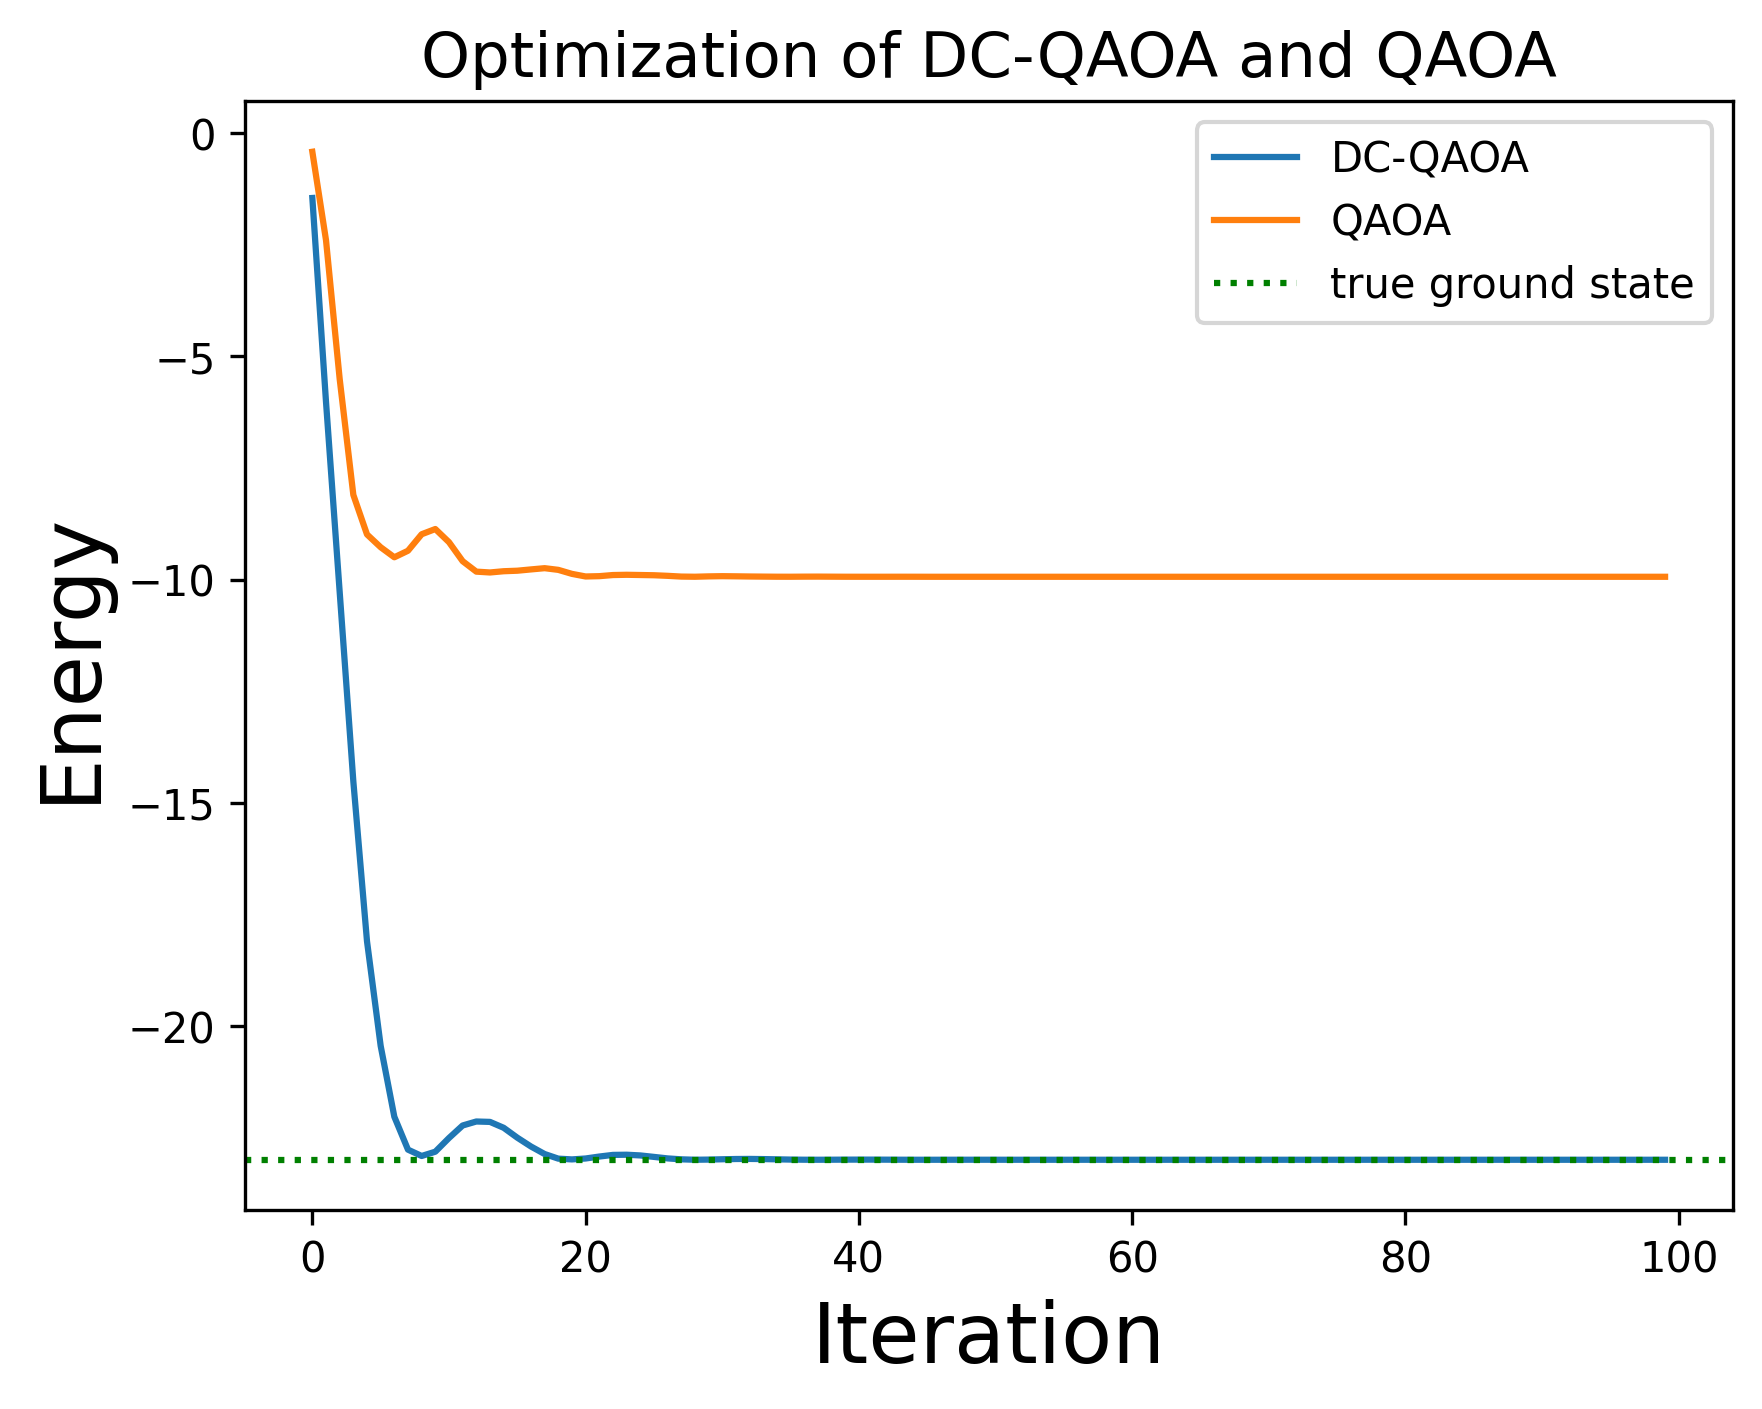
\includegraphics[width = 1 \linewidth]{5.4.1_figure/DC-QAOA.png}
    \caption{能量随迭代次数的变化。}
    \label{fig:dc}
\end{figure}


\subsection{对称增强 VQE}
查看本节演示代码：\demonotebook{05}{5.5_symmetry_enhanced_VQE} \ \demonotebookgithub{05}{5.5_symmetry_enhanced_VQE}

\subsubsection{背景}
变分量子算法主要聚焦于识别复杂多体系统的基态。在这一背景下，变分量子本征求解器（VQE）算法作为一种通过最小化平均能量来寻找多体系统基态的方法，已经成为强大工具。然而，物理中的若干关键现象（包括拓扑相）不仅需要了解基态，还需要了解多个低能本征态。因此，将 VQE 扩展到更高能量本征态具有重要意义。

加权 SSVQE 方法提供了另一种方案，用于生成给定哈密顿量 $H$ 的全部 $k$ 个最低能量本征态~\cite{nakanishi2019subspace}。该方法使用一组 $k$ 个正交初态，记为 $\{|\phi_{i}\rangle\}_{i=1}^{k}$（其中 $\langle \phi_{i} | \phi_{j} \rangle = \delta_{ij}$），作为单个参数化量子线路的输入，该线路由酉算符 $U(\vec{\theta})$ 描述。由于初态彼此正交，由同一线路生成的输出 $U(\vec{\theta})| \phi_{j} \rangle$ 也保持正交。在加权 SSVQE 中，目标是最小化代价函数
\begin{equation}
    \mathrm{cost} = \sum_{i=1}^{k} w_{i} \langle \phi_{i}| U^{\dagger}(\vec{\theta}) H U(\vec{\theta}) | \phi_{i} \rangle,
    \label{ssvqe_cost}
\end{equation}
其中 $w_1 > w_2 > \cdots > w_k$ 为正实数。最小化式~\eqref{ssvqe_cost} 中的代价函数会产生全部 $k$ 个最低能量本征态，使得 $|E_{i}\rangle = U(\vec{\theta}^{*})|\phi_{i}\rangle$。
加权 SSVQE 的一个显著优势是，它可以通过一次优化过程给出全部 $k$ 个最低能量本征态，而不需要评估量子态重叠。然而，随着目标本征态数量增加，该算法对资源的需求也会提高。

对称性是物理学，尤其是量子力学中最基本的概念之一。多数物理系统都表现出各种类型的对称性，并可通过数学方式准确描述。将这些对称性纳入 VQE 算法也能显著提升算法表现。将对称性引入 VQE 算法有两种方式：（i）设计能够自然生成具有相关对称性的量子态的线路~\cite{Lyu2020accelerated,Gard2020,barron2021preserving}；（ii）在代价函数中添加额外项，用于惩罚不具备相关对称性的量子态~\cite{mcclean2016theory,ryabinkin2018constrained}。

\subsubsection{实现}
利用 \MindQuantum\ 灵活且全面的功能，研究人员可以通过定义自定义目标函数来处理多种优化目标。本节演示如何使用 \MindQuantum\ 实现 SSVQE，并结合多种对称性策略，精确确定 Heisenberg 哈密顿量的四个最低态能量。

首先，需要构造保持对称性的 ansatz，详细内容见文献~\cite{Lyu2023symmetryenhanced}。
\begin{lstlisting}
def entangling_gate(parameter, qubits):
    circuit = Circuit()
    circuit += RZ(-np.pi / 2).on(qubits[1])
    circuit += CNOT.on(qubits[0], qubits[1])
    circuit += RZ({parameter: -2}).on(qubits[0])
    circuit += RZ(np.pi / 2).on(qubits[0])
    circuit += RY({parameter: 2}).on(qubits[1])
    circuit += RY(-np.pi / 2).on(qubits[1])
    circuit += CNOT.on(qubits[1], qubits[0])
    circuit += RY({parameter: -2}).on(qubits[1])
    circuit += RY(np.pi / 2).on(qubits[1])
    circuit += CNOT.on(qubits[0], qubits[1])
    circuit += RZ(np.pi / 2).on(qubits[0])
    return circuit

def ansatz(N, layers, local_rot=True):
    circuit = Circuit()
    params_index = 0
    for layer_index in range(layers):
        for i in range(2):
            for j in range(i, N - 1, 2):
                circuit += entangling_gate(str(params_index), [j, j + 1])
                params_index += 1
        if local_rot:
            for i in range(N):
                circuit += PhaseShift(params_index).on(i)
                params_index += 1
    return circuit
\end{lstlisting}

SSVQE 可以实现为多个 VQE 的组合，每个 VQE 具有不同初始化线路，但共享同一个参数化 ansatz。
对于多数 VQE 实例，具体任务由其对应测量函数定义。
使用 \getexpectationwithgrad\ 函数，可以方便地获得期望值及其关于可训练变量的对应梯度。这里以 Heisenberg 哈密顿量的第二和第三低能态能量为例，展示代码实现。在该具体实例中，
我们使用一个保持 $S_z$ 守恒的 ansatz，它保持总自旋的 $z$ 分量，并将总自旋算符作为惩罚项加入代价函数。代价函数随后修改为如下形式：
\begin{equation}
    \mathrm{cost} = \sum_{i=1}^{k} w_{i} \langle \phi_{i}| U^{\dagger}(\vec{\theta}) [H + \beta(\hat{O} - c)^2] U(\vec{\theta}) | \phi_{i} \rangle,
    \label{ssvqe_cost_pen}
\end{equation}
其中 $c$ 是表示目标子空间的常数，$\beta$ 是正的常数，其取值会根据惩罚项形式设置得足够大。这里展开 $(\hat{O} - c)^2 {=} \hat{O}^2 {-} c\hat{O} {+} c^2$。连同哈密顿量在内，我们现在有三个不同测量算符。Heisenberg 哈密顿量和总自旋算符情形下的相应测量算符可以通过以下代码生成。

\begin{lstlisting}
def s_alpha(N, alpha: str = 'X'):
    alpha = alpha.upper()
    out = QubitOperator()
    for i in range(N):
        out += QubitOperator(alpha + f'{i}')
    return out * 0.5

def s_tot_op(N):
    s_x_op = s_alpha(N, 'X')**2
    s_y_op = s_alpha(N, 'Y')**2
    s_z_op = s_alpha(N, 'Z')**2
    op = s_x_op + s_y_op + s_z_op
    op.compress()
    return op

def ham_heis(n_qubits, J):
    ham = QubitOperator()
    for i in range(1, n_qubits):
        ham += QubitOperator("X{} X{}".format(i - 1, i), J)
        ham += QubitOperator("Y{} Y{}".format(i - 1, i), J)
        ham += QubitOperator("Z{} Z{}".format(i - 1, i), J)
    ham.compress()
    return Hamiltonian(ham)
\end{lstlisting}

预先定义初始化线路、共享参数 ansatz、测量算符和常数 $\beta$ 等所有必要模块后，就可以继续实现 SSVQE 算法。以下代码片段展示了 SSVQE 类的实现。
\begin{lstlisting}
class SSVQE:
    def __init__(self, n_qubits, init_circuits, pqc, ops, beta):
        self.n_qubits = n_qubits
        self.circs = [circ + pqc for circ in init_circuits]
        self.sim = Simulator('mqvector', n_qubits)
        self.beta = beta
        self.grad_ops = [self.sim.get_expectation_with_grad(ops, circ) for circ in self.circs]

    def energy(self, params):
        if self.sim is None:
            self.sim = Simulator('mqvector', self.n_qubits)
        energies = []
        for i in range(len(self.grad_ops)):
            f, g = self.grad_ops[i](params)
            energies.append(f[0, 0].real)
        return energies

    def __call__(self, inputs):
        cost = 0
        cost_grad = 0
        for i in range(len(self.grad_ops)):
            f, g = self.grad_ops[i](inputs)
            f1, f2, f3 = f[0, 0].real, f[0, 1].real, f[0, 2].real
            g1, g2, g3 = np.array(g[0, 0, :].real), np.array(g[0, 1, :].real), np.array(g[0, 2, :].real)
            cost += (f1 + self.beta * (f2 + f3)) * (len(self.grad_ops) - i)
            cost_grad += (g1 + self.beta * (g2 + g3)) * (len(self.grad_ops) - i)
        return cost, cost_grad
\end{lstlisting}


完成算法实现后，重点转向 SSVQE 优化。经典优化器的选择仍然是灵活的。在本例中，选择 SciPy 中的 \code{"L-BFGS-B"} 优化器。


\begin{lstlisting}
initial_parameter = (np.random.rand(len(ssvqe.circs[0].params_name)) - .5) * np.pi
res = scipy.optimize.minimize(ssvqe,
                    initial_parameter,
                    method='l-bfgs-b',
                    jac=True,
                    options={'disp': False})
\end{lstlisting}

\begin{figure}
	\centering
	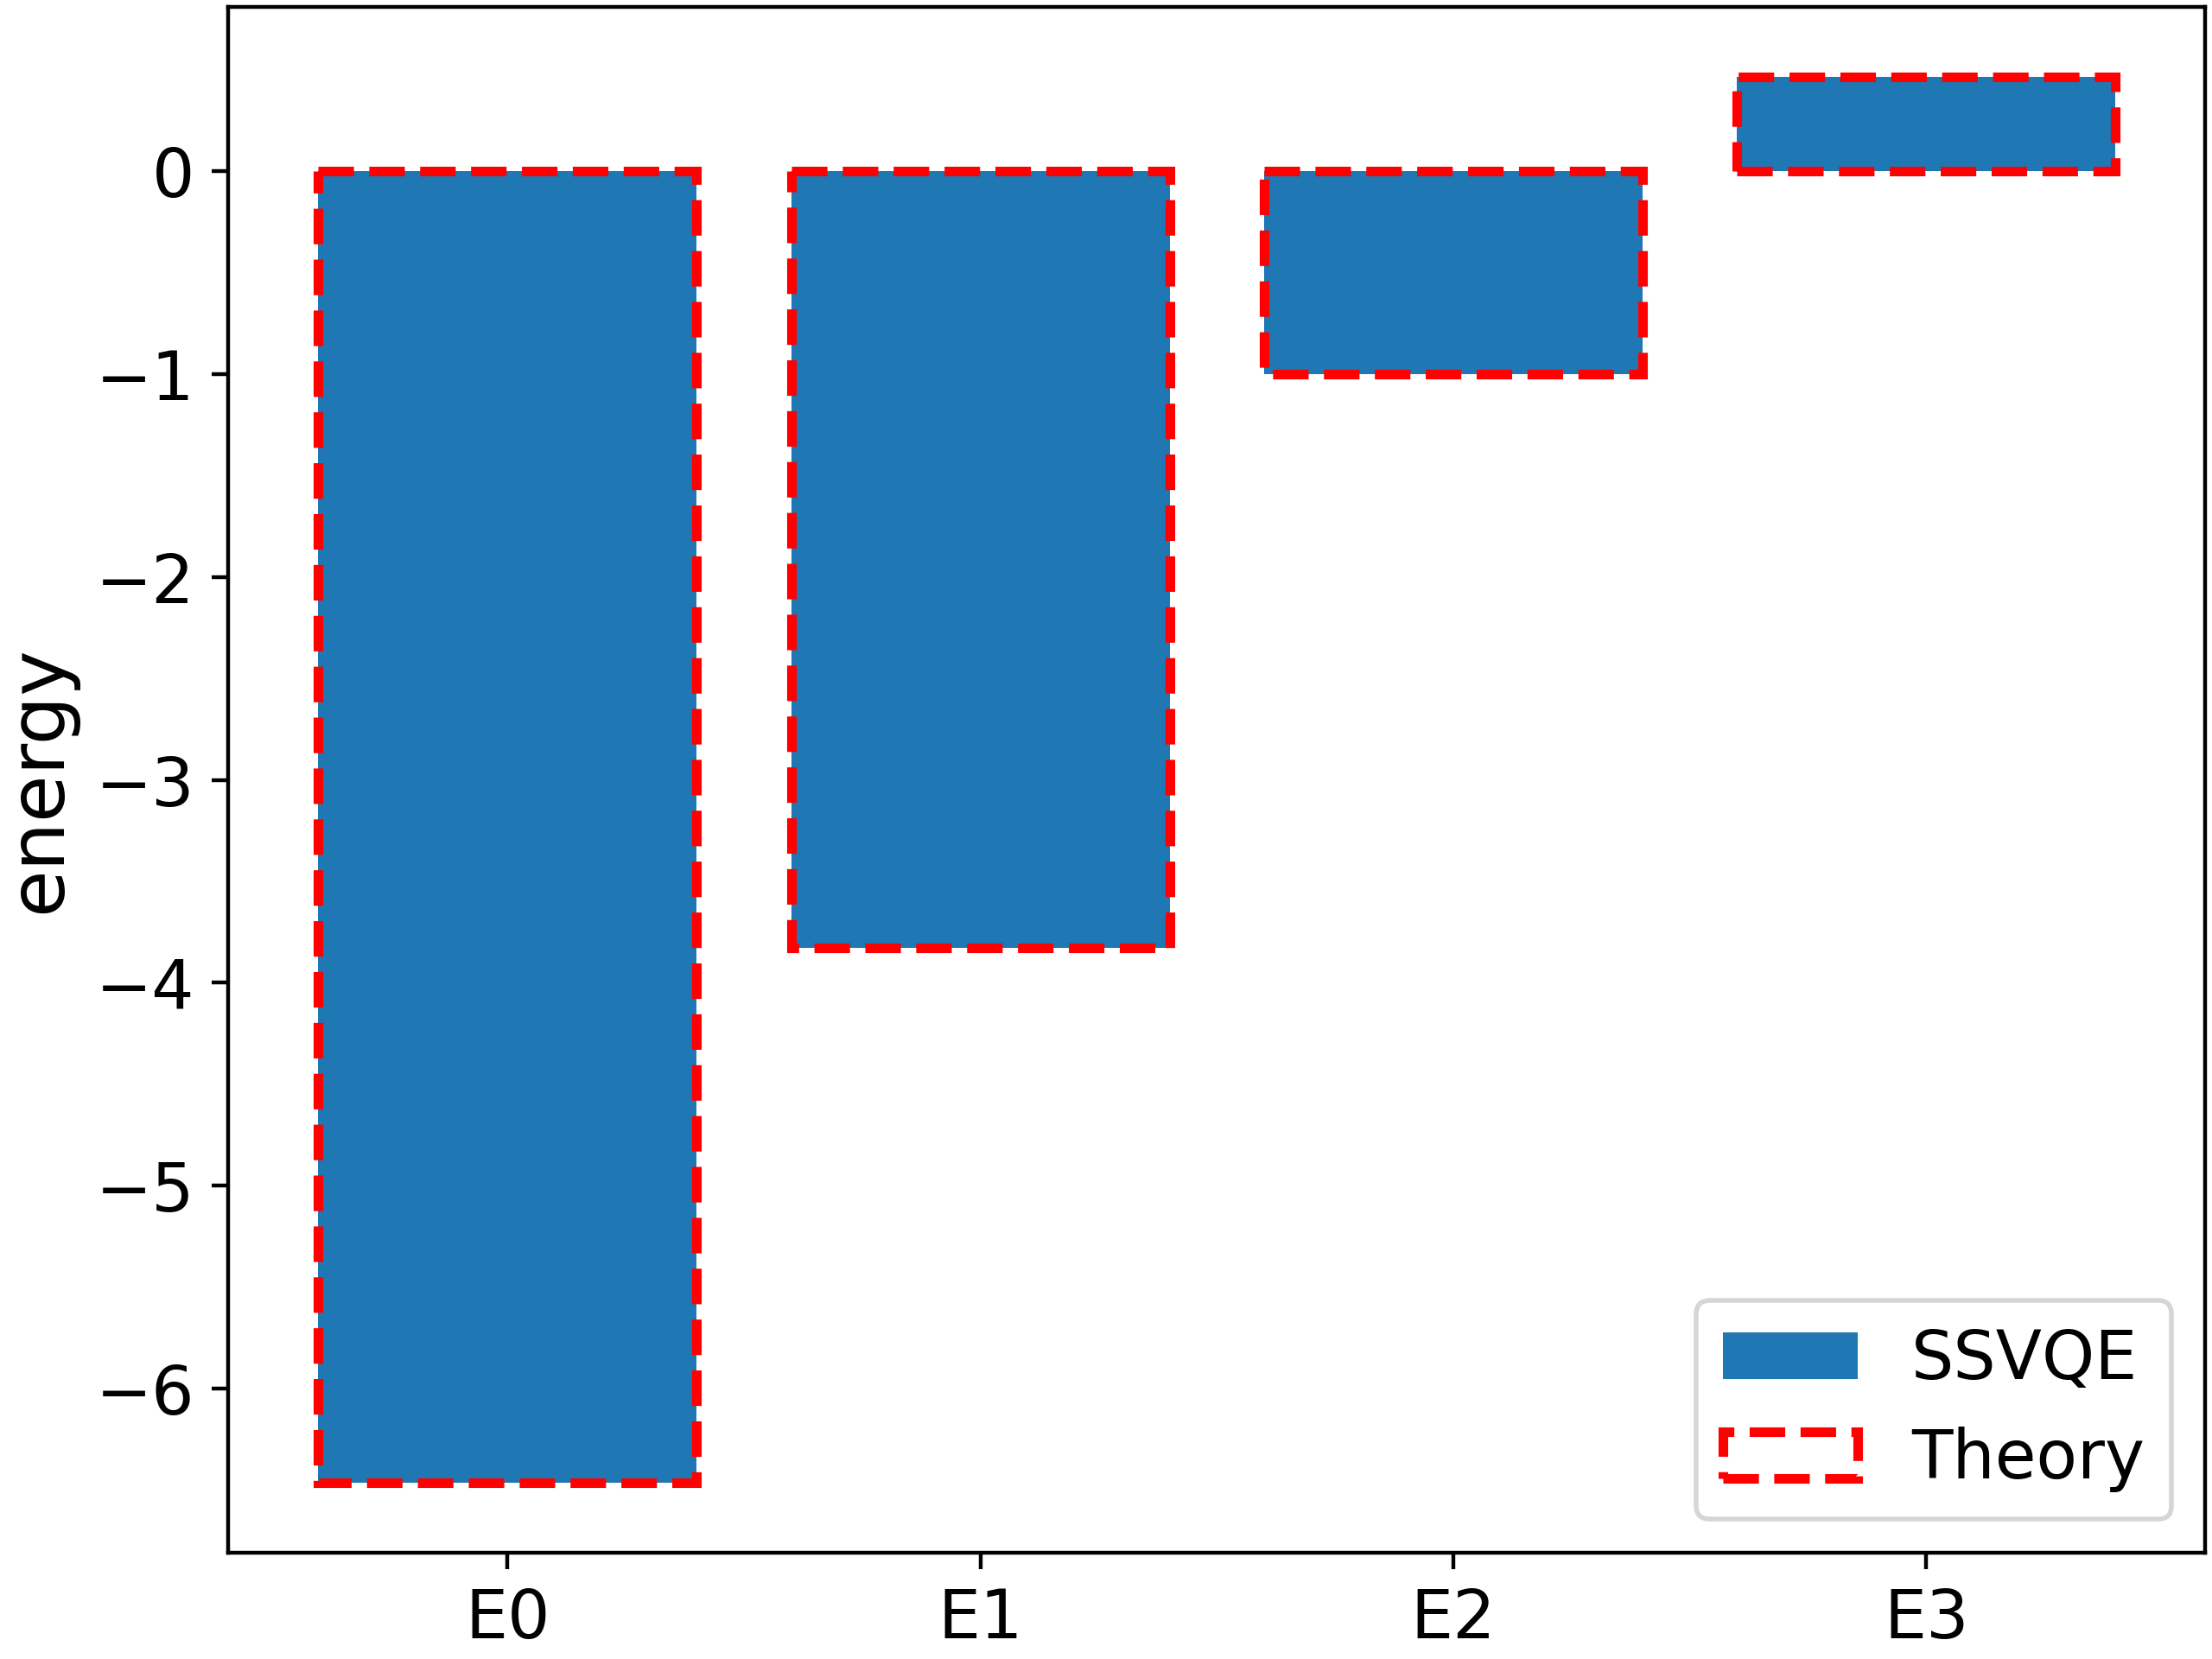
\includegraphics[width=1\linewidth]{5.4.2_figure/result.png}
	\caption{结合对称性的 SSVQE 在 4 量子比特 Heisenberg 哈密顿量上的模拟结果}
	\label{fig:SSVQE_result}
\end{figure}

该实现只需数秒即可完成 4 量子比特 Heisenberg 哈密顿量的训练。可以查看最终结果，并生成图像比较近似结果与理论能量。图~\ref{fig:SSVQE_result} 展示了 $4$ 量子比特 Heisenberg 哈密顿量四个最低态能量的模拟结果。显然，通过在 SSVQE 中纳入内在对称性，可以以资源高效的方式精确近似基态和激发态能量。


\subsection{数据重上传分类器}
\input{5.4.3_Data-reuploading_Classifier}

\subsection{Q-GAN}
查看本节演示代码：\href{https://gitee.com/mindspore/mindquantum/blob/research/paper_with_code/variational_quantum_circuits_enhanced_generative_adversarial_network/QGAN.py}{\color{ceruleanblue}{Gitee}} \ \href{https://github.com/donghufeng/mindquantum_tutorial_code/blob/master/whitepaper/code/chapt05/5.7_Q-GAN/QGAN.py}{\color{ceruleanblue}{GitHub}}

\subsubsection{背景}
生成对抗网络（Generative Adversarial Network, GAN）是 Goodfellow 提出的一类著名机器学习模型。它在多种具有挑战性的任务中表现突出，尤其适用于图像生成和视频生成。一般的 GAN 由生成器 ${G}$ 和判别器 ${D}$ 组成，并通过 ${G}$ 与 ${D}$ 之间的对抗博弈完成生成任务。在训练过程中，${G}$ 的目标是最大化 ${D}$ 将生成数据误判为真实数据的概率；相应地，${D}$ 的目标是最大化其正确识别真实数据的概率，同时最小化其将生成数据误判为真实数据的概率。GAN 的目标函数可概括为
\begin{equation}
  \begin{split}
    \mathop {\min }\limits_G \mathop {\max }\limits_D V(D,G) = {\rm{ }}{{\rm{E}}_{x\sim{p_r}(x)}}[\log D(x)]
    \\+ {{\rm{E}}_{z\sim{p_z}(z)}}[\log (1 - D(G(z)))]. \label{eq1}
  \end{split}
\end{equation}

QGAN 作为 GAN 的量子版本，在采样和生成离散数据方面比经典对应模型具有更多优势。此外，理论上已经证明其具备潜在的指数加速能力 \cite{lloyd2018quantum}。这些优势推动了围绕 QGAN 的大量研究，例如经典或量子数据学习 \cite{benedetti2019adversarial, zeng2019learning, zoufal2019quantum,ahmed2021quantum}、利用量子线路纠缠能力克服非凸性和模式崩塌问题 \cite{niu2022entangling}、小分子药物发现 \cite{li2021quantum}、数据增强 \cite{nakaji2021quantum}，以及基于 QGAN 的异常检测 \cite{herr2021anomaly}。

\subsubsection{实现}
本节展示如何使用 \MindQuantum\ 构建一个混合量子-经典生成对抗网络（QC-GAN）\cite{shu2024variational}，并通过训练学习一个概率分布，从而生成手写数字。具体而言，QC-GAN 使用一个变分量子线路和一层神经网络组成 ${G}$，并使用经典神经网络组成 ${D}$。其训练方式与经典 GAN 类似：将噪声向量 ${z}$ 输入 ${G}$，随后通过 ${G}$ 和 ${D}$ 的对抗训练实现图像生成。
不同之处在于，生成图像由量子线路演化、测量以及神经网络的非线性映射共同得到。QC-GAN 的整体结构和训练过程如图 \ref{qc-gan} 所示。

\begin{figure}[ht]
  \centering
  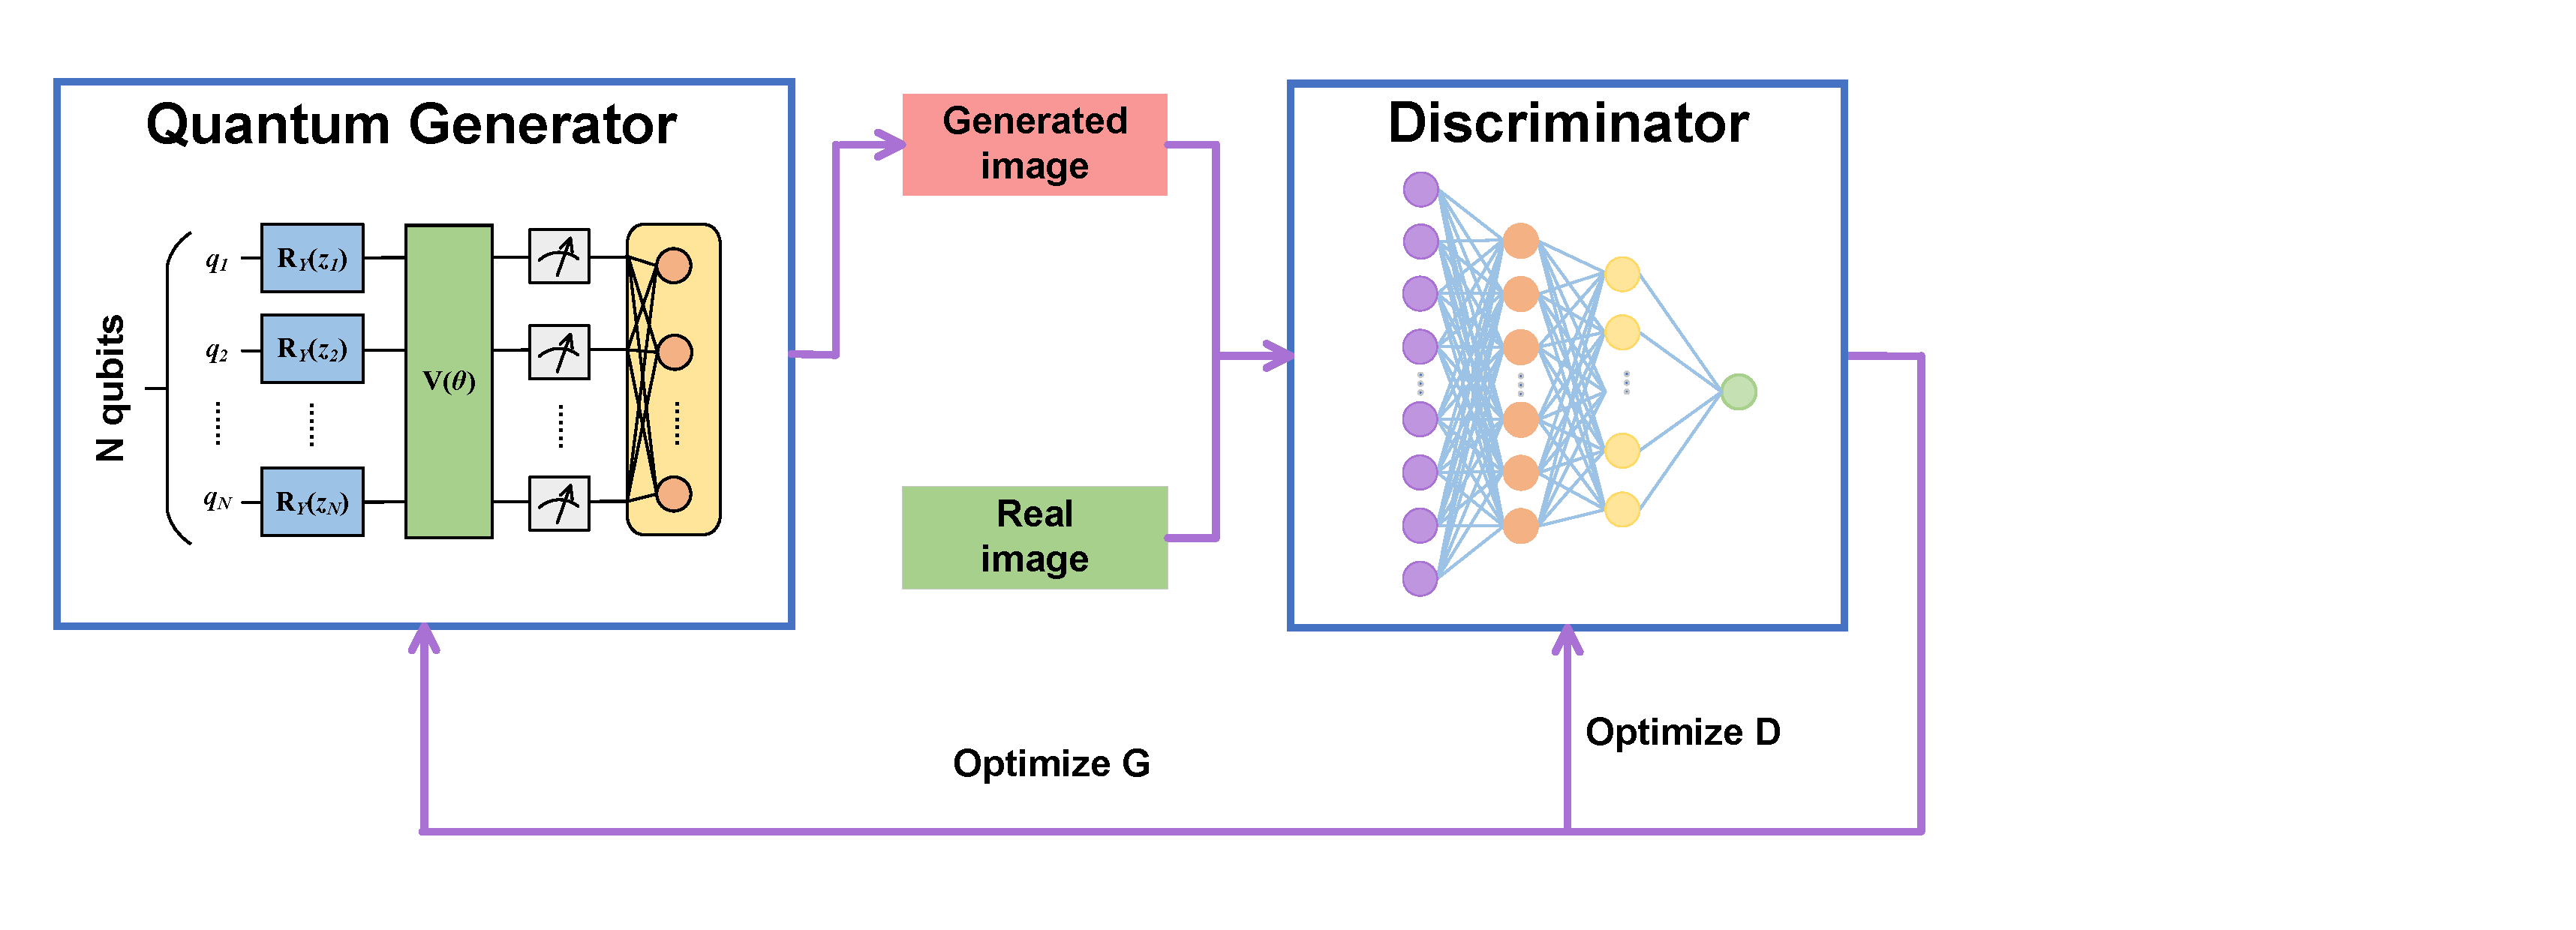
\includegraphics[scale=0.2]{5.4.4_figures/qc-gan.pdf}
  \caption{\label{qc-gan} QC-GAN 的整体架构与训练过程。}
\end{figure}

第一步是加载数据集。实验使用手写数字数据集，该数据集共有 70,000 张手写数字图像，其中包含 60,000 个训练样本和 10,000 个测试样本；图像尺寸为 28*28，且为单通道图像。加载数据集后，需要执行一系列预处理操作，为后续训练做准备。模型构建部分由两个网络组成，即生成器 ${G}$ 和判别器 ${D}$。判别器部分采用常规全连接网络结构。生成器则分为量子部分和经典部分。量子线路通过调用 \MindQuantum\ 的参数化旋转门构建，具体如下。量子线路结构可以通过 \Circuit\ 的 \methodsummary 方法展示。
\begin{figure*}[htbp]
  \centering
  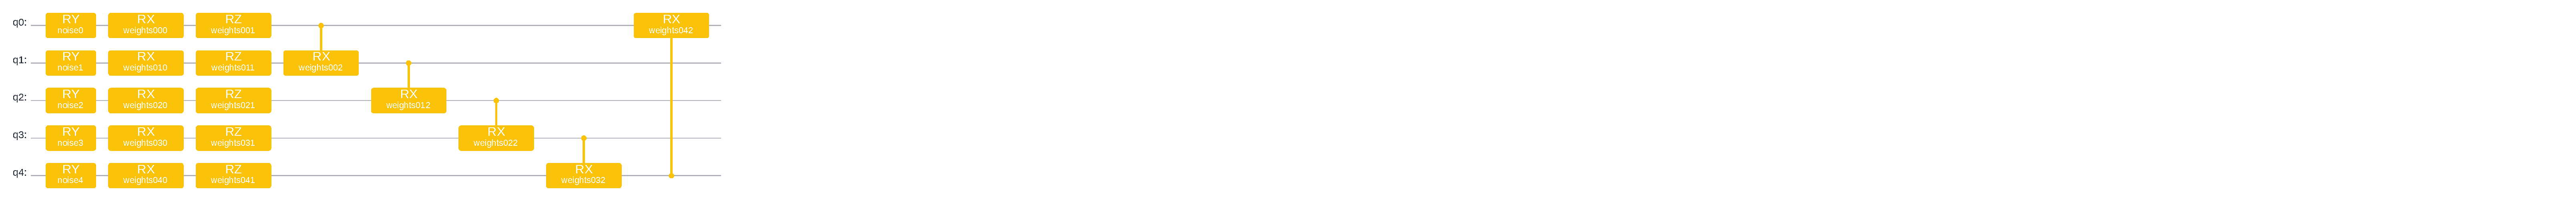
\includegraphics[scale=0.5]{5.4.4_figures/circuit.pdf}
  \caption{\label{quantum-circuit} 量子线路。}
\end{figure*}

\begin{lstlisting}
def quantum_circuit():
  encoder = Circuit()
  for i in range(qubits):
      encoder += RY(f'noise{i}').on(i)
  encoder = encoder.no_grad()
  ansatz = Circuit()
  for i in range(depth):
      for k in range(gate):
          for j in range(qubits):
              if k == 0:
                  ansatz += RX(f'weights{i}{j}{k}').on(j)
              elif k == 1:
                  ansatz += RZ(f'weights{i}{j}{k}').on(j)
              elif k == 2:
                  if j < 4:
                      ansatz += RX(f'weights{i}{j}{k}').on(j + 1, j)
                  else:
                      ansatz += RX(f'weights{i}{j}{k}').on(0, j)
  circuit = encoder.as_encoder() + ansatz.as_ansatz()
  return circuit
\end{lstlisting}
将量子线路按层堆叠并测量输出，即可构成一个量子层。
\begin{lstlisting}
def quantum_layer(qubits):
    circuit = quantum_circuit()
    circ_l = Circuit()
    hams = quantum_measure(qubits)
    sim = Simulator('mqvector', circuit.n_qubits)
    sim_l = Simulator('mqvector', qubits)
    grad_ops = sim.get_expectation_with_grad(hams, circuit, circ_l, sim_l, parallel_worker=4)

    QuantumNet = MQLayer(grad_ops,
                         weight=ms.Tensor(np.random.uniform(-np.pi, np.pi, len(circuit.ansatz_params_name)),
                         dtype=ms.dtype.float32))
    return QuantumNet
\end{lstlisting}

随后，与构建经典神经网络类似，定义网络的各个层并设置前向传播过程，即可组成量子生成器模型。反向传播过程会自动求导并更新参数。
\begin{lstlisting}
  class QuantumGenerator(nn.Cell):
    def __init__(self):
        super(QuantumGenerator, self).__init__()
        self.quantumlayer = quantum_layer(qubits)
        self.linear = nn.Dense(2**qubits, img_size * img_size, weight_init='uniform')
        self.relu = nn.ReLU()
        self.sigmoid = nn.Sigmoid()
        self.tanh = nn.Tanh()

    def construct(self, x):
        x = self.quantumlayer(x)
        x = x/(abs(x).max())
        x = self.linear(x)
        out = self.sigmoid(x)
        return out
\end{lstlisting}

量子线路参数会依据所设计的代价函数进行优化。生成器需要生成尽可能接近真实样本的概率分布，判别器则需要尽可能区分真实分布与生成分布。二者的代价函数分别设计如下。
\begin{equation}
  {L_G} =  - {{\rm E}_{x\sim{p_f}(x)}}\left[ {\log D(x)} \right],
\end{equation}
\begin{equation}
  {L_D} =  - {{\rm E}_{x\sim{p_r}(x)}}\left[ {\log D(x)} \right] - {{\rm E}_{x\sim{p_f}(x)}}\left[ {\log D(x)} \right].
\end{equation}

根据设计好的损失函数和模型，生成器与判别器会交替训练并更新参数。训练完成后，将噪声向量作为生成器输入，即可输出生成的手写数字，结果如图 \ref{qgan-result} 所示。可以看到，随着迭代次数增加，输入噪声逐渐能够生成清晰的数字图像。需要注意的是，训练迭代次数必须谨慎设计，并非越多越好。
\begin{figure}[htbp]
  \centering
  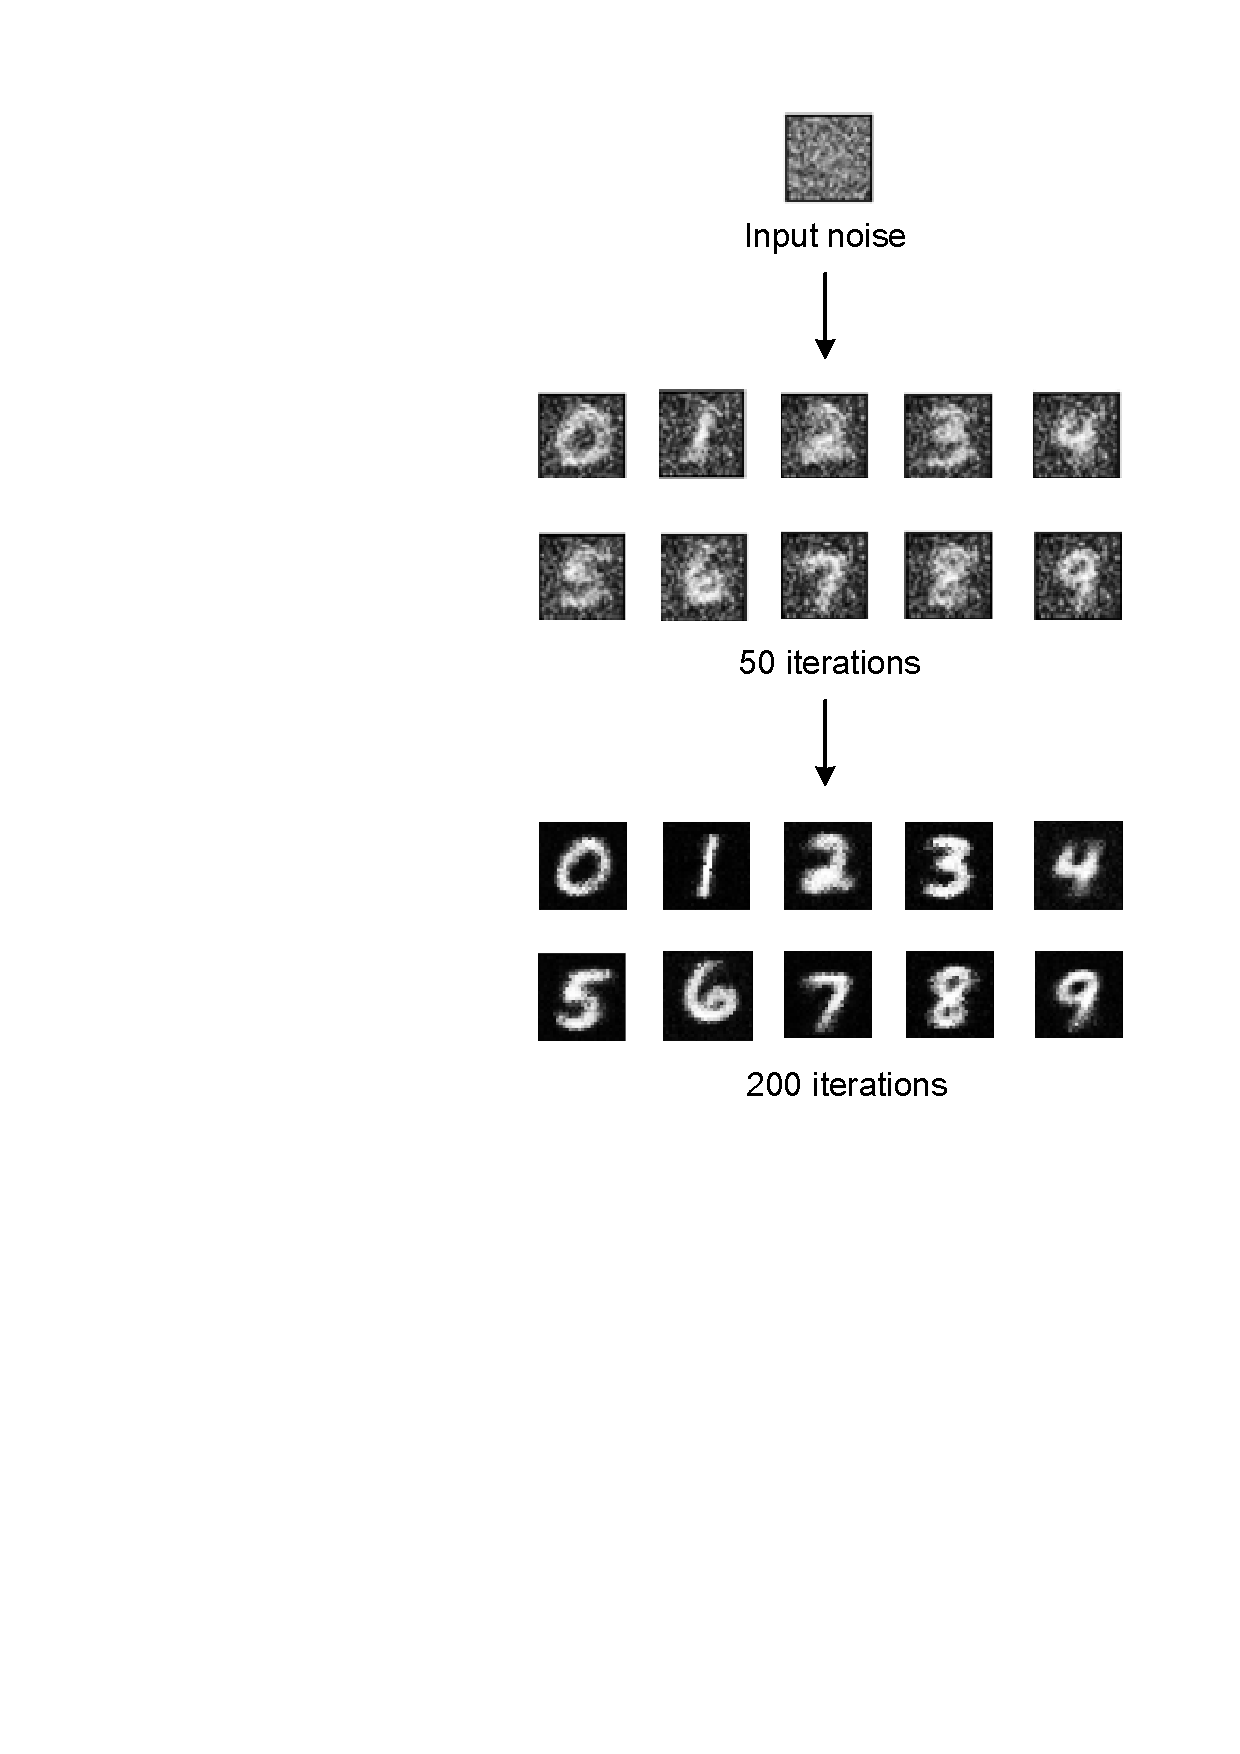
\includegraphics[scale=0.5]{5.4.4_figures/qgan-result.pdf}
  \caption{\label{qgan-result} QC-GAN 在不同训练阶段生成的手写数字结果。}
\end{figure}


\subsection{强化学习}
查看本节演示代码：\democode{05}{5.8_Reinforcement_Learning} \ \democodegithub{05}{5.8_Reinforcement_Learning}

\subsubsection{背景}

一个完整的强化学习算法（Reinforcement Learning, RL）由智能体（Agent）、环境（Environment）、状态（State）、动作（Action）和奖励（Reward）组成。智能体执行一个动作后，环境会根据该动作转移到新的状态，并依据一定规则给出奖励。随后，智能体根据获得的新状态和奖励更新其决策过程并给出新的动作，如此循环，直到整个控制过程完成 \cite{kaelbling1996reinforcement}。我们用 $\pi_{\theta}$ 表示策略函数，$s$ 表示环境的每个状态，$r$ 表示每个状态中的奖励，$a$ 表示智能体的动作。RL 的架构如图 \ref{RL_frame} 所示。
\begin{figure}[ht]
  \centering
  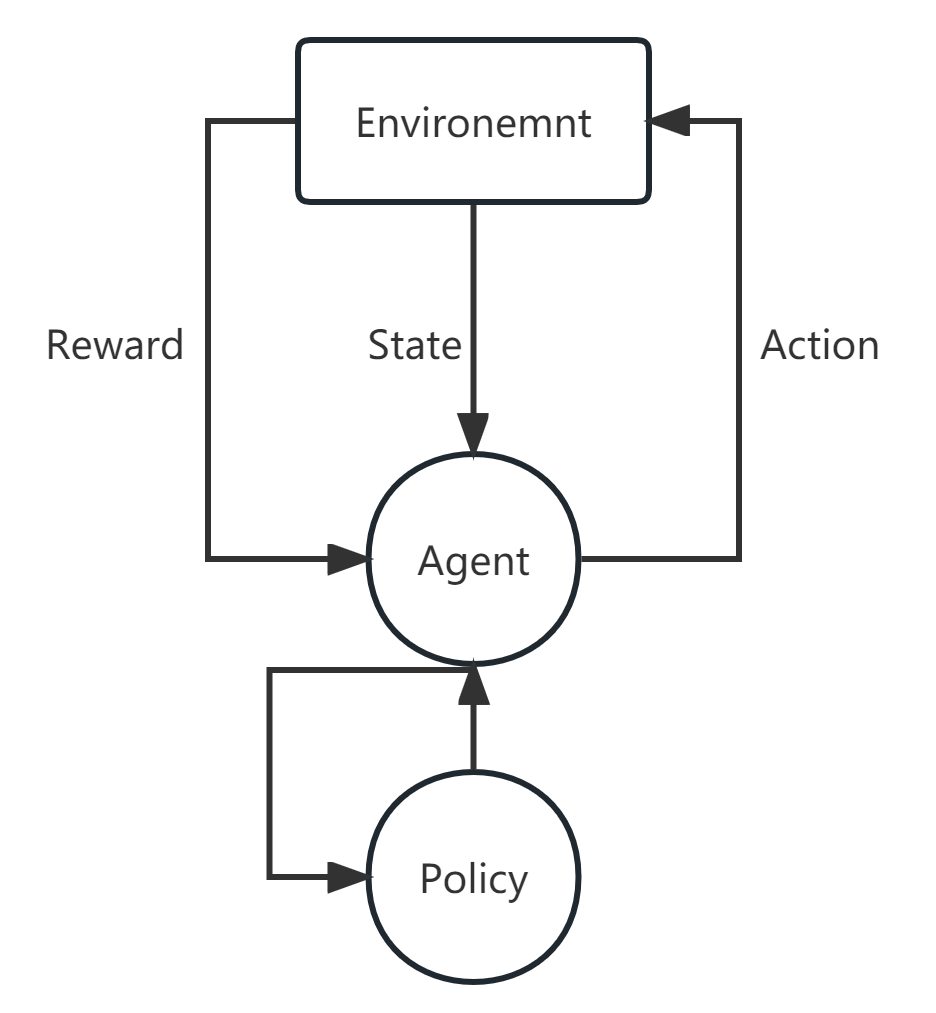
\includegraphics[scale=0.4]{5.4.5_RL/RL.png}
  \caption{\label{RL_frame} RL 工作流程示意图。}
\end{figure}

假设一个环境包含 $N$ 个不同状态。我们在状态 $s_{i-1}$ 上执行动作 $a_{i-1}$，并得到结果状态 $s_i$。从状态 $s_i$ 在动作 $a_i$ 下转移到状态 $s_{i+1}$ 的转移概率函数可以写为 $P(s_{i+1}|s_i,a_i)$。同时，每个状态中都有一个由奖励函数 $R_i=R(a_i,s_i,s_{i-1})$ 计算得到的奖励 $r_i$。在环境变化过程中，如果奖励期望只由最新的 $state$ 决定，则称其为马尔可夫决策过程。因此，智能体选择每条 $T$ 步轨迹的概率为：

\begin{equation}
    \begin{split}
        &P(\tau|\pi_{\theta})=\\
        &\rho(s_0)\prod_{k=0}^{k=T-1}P(s_{k+1}|s_{k},a_{k})\pi_{\theta}(a_{k}|s_{k}),
    \end{split}
\end{equation}
其中 $\rho$ 是初始状态分布。于是，$T$ 步轨迹奖励的期望为：
\begin{equation}
    \eta(\pi_{\theta})=\int_{\tau}P(\tau|\pi_{\theta})R(\tau)d\tau.
\end{equation}
为了得到最优策略函数 $\pi_{\theta}$，需要训练智能体来最大化期望 $\eta$，即：
\begin{equation}
    \pi_{\theta}^{opt}=\mathrm{argmax}_{\theta}\eta(\pi_{\theta}).
\end{equation}
在后续部分中，我们将展示如何在量子设备上训练智能体。

\subsubsection{混合深度 Q 网络}

用量子变分线路替换经典深度 Q 网络智能体中的神经网络，即可得到混合深度 Q 网络（Hybrid Deep Q-Network, HDQN）\cite{Q_rl}。HDQN 的架构如图 \ref{HDQN} 所示。

\begin{figure*}[ht]
    \centering
    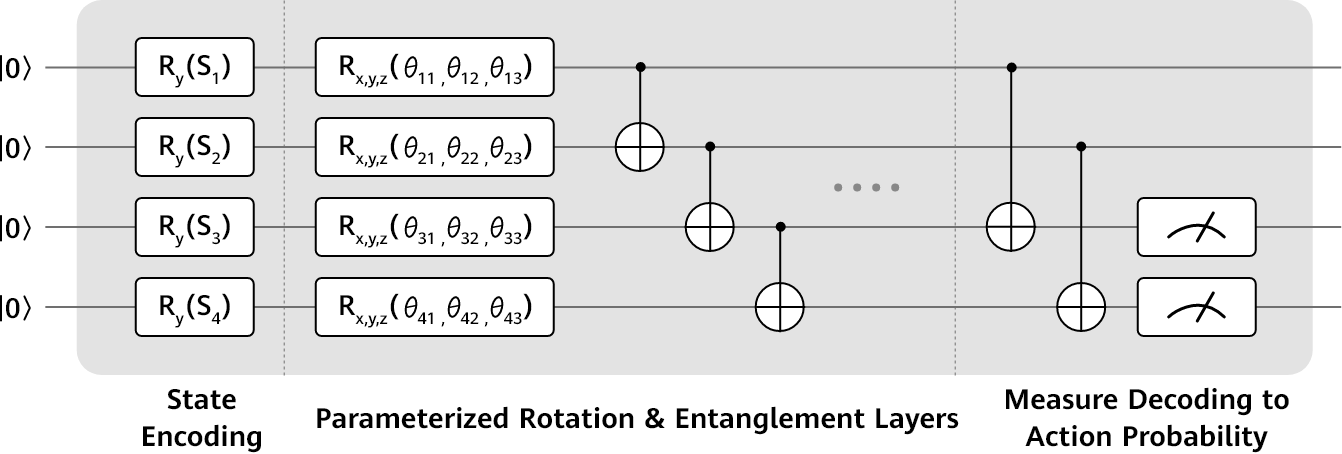
\includegraphics[width=0.9\linewidth]{5.4.5_RL/HDQN.png}
    \caption{\label{HDQN} HDQN 架构。}
  \end{figure*}

我们通过经典神经网络计算参数 $\theta$，并用这些参数构造量子变分线路。最终，量子部分会向环境施加动作，同时环境返回奖励 $r_i$。记 $e_i=(s_i,a_i,r_{i+1},s_{i+1})$ 为一条经验。在训练阶段，我们会把这些经验作为训练样本，并依据损失函数 $L(\theta)$ 调整经典部分和量子部分中的参数：
\begin{equation}
\begin{split}
    L(\theta_{j})=&E[R_{i+1}+\\
    &\gamma \max_{\alpha^{'}}Q(s_{i+1},a^{'},\theta_{j}^{-})-Q(s_{i},a_{i},\theta_{i})^2].
\end{split}
\label{loss func}
\end{equation}

\textit{变分量子线路} -- 变分量子线路是一类使用可调参数的量子线路，这些参数可以随外部环境改变。在这里，我们根据文献 \cite{Q_rl} 中的架构，采用 encoder 与 ansatz 组合的方式构造量子线路。其中，ansatz 采用 Hardware Efficient 线路。整体量子线路如图 \ref{Agent_qc} 所示。

\begin{figure*}[ht]
  \centering
  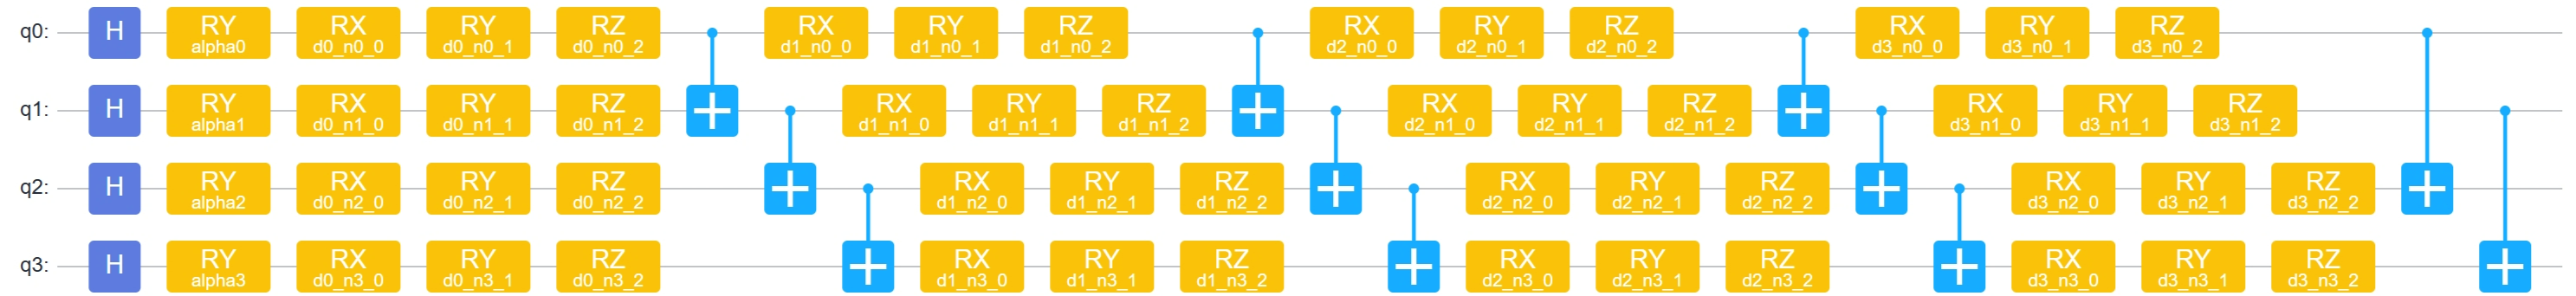
\includegraphics[scale=0.5]{5.4.5_RL/Circuit.png}
  \caption{\label{Agent_qc} RL 智能体的整体量子线路。}
\end{figure*}

\textit{MindQuantum 中的实现} -- 这里给出使用 \MindQuantum\ 实现 HDQN 的示例。第一步是构造包含 encoder 和 ansatz 的量子变分线路。
\begin{lstlisting}
def __get_encoder(self):
    encoder = Circuit()
    encoder += UN(H, 4)
    for i in range(4):
        encoder += RY(f'alpha{i}').on(i)
    encoder = encoder.no_grad()
    # 无梯度量子线路: no_grad()
    encoder.summary()
    return encoder
def __get_ansatz(self):
    ansatz = HardwareEfficientAnsatz\\
        (4, single_rot_gate_seq=[RX,RY,RZ],\\
        entangle_gate=X, depth=3).circuit
    ansatz += X.on(2,0)
    ansatz += X.on(3,1)
    ansatz.summary()
    return ansatz
self.circuit = self.encoder + self.ansatz
\end{lstlisting}

经过量子线路处理后，我们需要构造一个可观测量哈密顿量作为测量基。这里仅在 $\sigma_y$ 基上测量第二个和第三个量子比特。哈密顿量如下：
\begin{equation}
    H=I\otimes I\otimes\sigma_y\otimes\sigma_y.
\end{equation}
我们可以用 \MindQuantum\ 按如下方式构造该哈密顿量：
\begin{lstlisting}
def __get_observable(self):
    hams=[Hamiltonian(QubitOperator(f'Y{i}'))\\
        for i in [2, 3]]
    return hams
\end{lstlisting}
此外，通过 \getexpectationwithgrad 函数可以方便地获得期望值并计算期望值梯度，该梯度可用于优化参数。

接下来，需要实现经典部分，即一个带激活函数的三层全连接神经网络。
\begin{lstlisting}
class Critic(nn.Cell):
    def __init__(self):
        super(Critic, self).__init__()
        self.relu = nn.ReLU()
        self.fc1 = nn.Dense(4, 64)
        self.fc2 = nn.Dense(64, 256)
        self.fc3 = nn.Dense(256, 1)

    def construct(self, x):
        x = self.relu(self.fc1(x))
        x = self.relu(self.fc2(x))
        x = self.fc3(x)
        return x
\end{lstlisting}

\textit{环境} -- 这里关注 gym 游戏 \code{"CartPole-v0"}。该游戏中有一辆在轨道上运动、上方竖立着摆杆的小车。游戏有两个输入 $0$ 和 $1$，分别对应向左和向右两个方向。用户需要控制小车沿这两个方向移动，并尽可能长时间地保持摆杆平衡。

第一步是通过 gym 创建环境。
\begin{lstlisting}
import gym
env = gym.make('CartPole-v0')
\end{lstlisting}
\textit{记忆缓冲区} -- 在训练过程中，训练样本会从之前的经验 $e_i$ 中随机选取。因此，需要构造一个缓冲区来存储并采样经验 $e_i$。
\begin{lstlisting}
class Memory(object):
    ......
\end{lstlisting}

完整实现可见于本节开头给出的示例代码。

\subsubsection{训练}
最后一步是模型训练。首先，用随机参数初始化 HDQN，并让 actor 与环境交互。然后，将交互结果存入记忆缓冲区，作为训练样本。最后，从记忆缓冲区采样，并利用损失函数（\ref{loss func}）同时调整经典部分和量子部分的参数。受篇幅限制，这里不再给出详细代码。

\textit{数值模拟结果} -- 为了评估 HDQN 的效果，我们进行了若干实验。图 \ref{stochastic} 展示了多次实验的平均结果与随机策略实验之间的比较。结果表明，以量子线路作为智能体的强化学习模型确实学习到了策略。
\begin{figure}[ht]
  \centering
  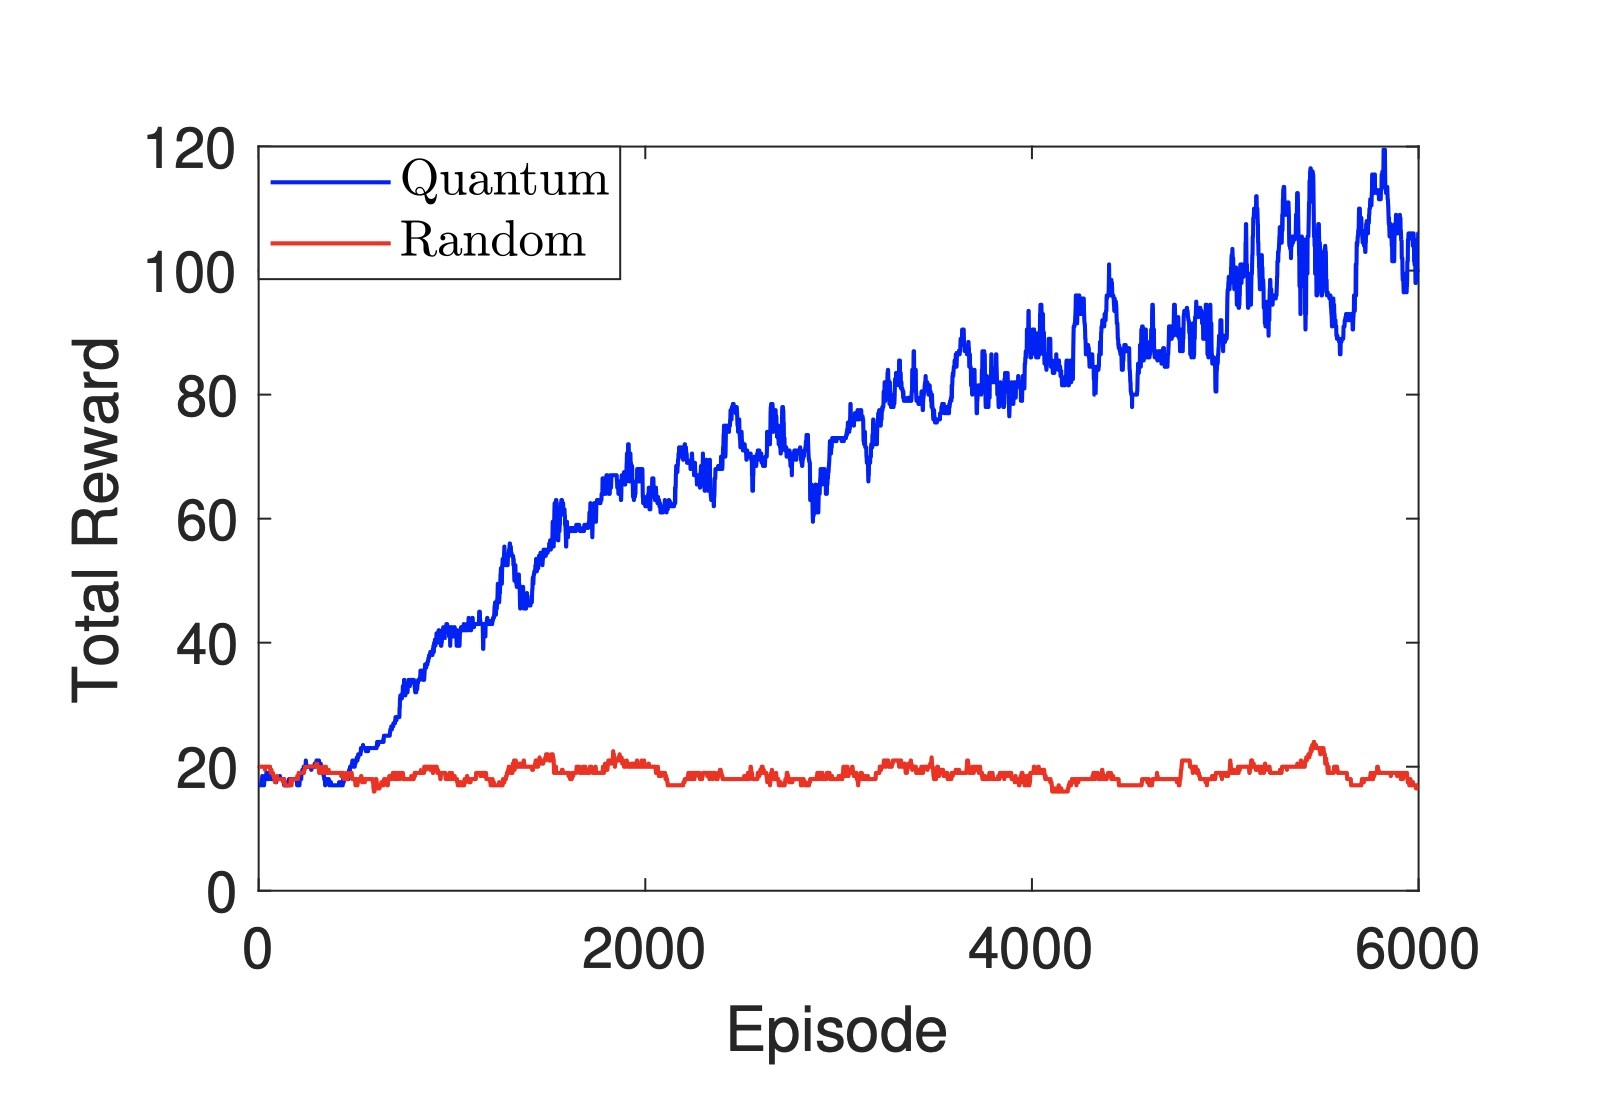
\includegraphics[scale=0.3]{5.4.5_RL/result_paper.jpg}
  \caption{\label{stochastic} RL 与随机策略的比较。}
\end{figure}


\subsection{量子奇异值分解}
查看本节演示代码：\democode{05}{5.9_Quantum_Singular_Value_Decomposition} \ \democodegithub{05}{5.9_Quantum_Singular_Value_Decomposition}

\subsubsection{背景}
奇异值分解（Singular Value Decomposition, SVD）是线性代数中一种重要的矩阵分解。作为任意维矩阵上特征分解的推广，SVD 被广泛用于机器学习领域，包括矩阵压缩、推荐系统和自然语言处理等。其定义如下：
给定复矩阵 $M \in \mathbb{C}^{m \times n}$，矩阵 $M$ 的 SVD 定义为 $M = UDV^\dagger$。其中，$U$ 是 $m \times m$ 酉矩阵，$V$ 是 $n \times n$ 酉矩阵，即满足 $UU^\dagger = I$、$VV^\dagger = I$。$D$ 是一个 $m \times n$ 对角矩阵，其主对角线元素通常按从大到小排列，每个元素称为矩阵 $M$ 的一个奇异值。


已有工作提出了用于 SVD 的量子算法 \cite{kerenidis2016quantum, rebentrost2018quantum}，并进一步带来了求解线性方程组 \cite{wossnig2018quantum} 和开发量子推荐系统 \cite{kerenidis2016quantum} 等应用。然而，这些算法的资源开销过高，难以在近期量子设备上得到有说服力的验证。当前使用含噪中等规模量子（NISQ）设备求解各类问题的主流策略称为变分量子算法。

针对奇异值分解，文献 \cite{wang2021variational} 提出了一种变分量子算法（VQSVD），其思想是把 SVD 任务表述为一个优化问题。VQSVD 算法的详细流程如下：
\begin{enumerate}
    \item 准备 VQSVD 算法的输入：
        \begin{itemize}
            \item 将矩阵 $M$ 分解为 $K$ 个酉矩阵的线性组合，形式为 $M = \sum_{k=1}^K c_k A_k$，其中 $c_k$ 为实数。
            \item 正权重 $q_1 > \cdots > q_r > 0$。
            \item 计算基 {$\ket{\psi_1}, \cdots, \ket{\psi_T}$}，其中 $T$ 是期望秩。
            \item 参数化线路 $U(\theta)$、$V(\phi)$ 及其初始参数 $\theta, \phi$。
        \end{itemize}
    \item 进入混合量子-经典优化循环，训练参数化量子线路 $U(\theta)$ 和 $V(\phi)$ 中的参数 $\theta$ 与 $\phi$，并计算 $M$ 的奇异值：$m_j = \text{Re}\langle\psi_j|U(\theta)^{\dagger} M V(\phi)\ket{\psi_j}$。优化目标是最大化设计好的损失函数 $L(\theta, \phi)$：
    \begin{equation}
        L(\theta, \phi) = \sum_{j=1}^T q_j \times \text{Re} \langle\psi_j| U(\theta)^{\dagger} M V(\phi)\ket{\psi_j},
    \end{equation}
    其中引入权重是为了使计算得到的奇异值按降序排列。
    \item 获得最优参数 $\alpha^ \star$ 和 $\beta^\star$，并计算 $U(\alpha^\star)$ 与 $V(\beta^\star)$。
    \item 获得近似奇异值 ${m_1, \cdots, m_r}$，以及奇异向量 $U(\alpha^\star)$ 和 $V(\beta^\star)$。
\end{enumerate}

\subsubsection{实现} -- 本节展示如何使用 \MindQuantum\ 分解一个随机生成的 $8 \times 8$ 复矩阵。

首先需要引入所需软件包，定义必要常数并设置权重，然后使用 \code{numpy.random.randint} 函数随机生成一个 $8 \times 8$ 复矩阵 $M$：
\begin{lstlisting}
from mindquantum import Simulator, MQAnsatzOnlyLayer, add_prefix
from mindquantum import Hamiltonian, Circuit, RY, RZ, X
import mindspore as ms
import numpy as np
from scipy.sparse import csr_matrix
from scipy.linalg import norm
from matplotlib import pyplot
import tqdm

n_qubits = 3  # 量子比特数
cir_depth = 20  # 线路深度
N = 2**n_qubits
rank = 8  # 学习秩
step = 3
ITR = 200  # 迭代次数
LR = 0.02  # 学习率

# 设置等间隔学习权重
if step == 0:
    weight = ms.Tensor(np.ones(rank))
else:
    weight = ms.Tensor(np.arange(rank * step, 0, -step))

# 定义随机种子
np.random.seed(42)

def mat_generator():
    '''
    生成随机复矩阵
    '''
    matrix = np.random.randint(
        10, size=(N, N)) + 1j * np.random.randint(10, size=(N, N))
    return matrix

# 生成待分解矩阵 M
M = mat_generator()
# 生成 m_copy 用于误差分析
m_copy = np.copy(M)
print('Random matrix M is: ')
print(M)
# 获得 SVD 结果
U, D, v_dagger = np.linalg.svd(M, full_matrices=True)
\end{lstlisting}

接下来，定义仿真中用于 $U(\theta)$ 和 $V(\phi)$ 的硬件高效 ansatz，即论文 \cite{wang2021variational} 中使用的变分 ansatz。由于这里只涉及实矩阵，旋转门与 CNOT 的组合已经足够。在该 ansatz 中，每个相同模块（虚线框所示）由一列绕 $y$ 轴和 $z$ 轴的单量子比特旋转门，以及随后一层只连接相邻量子比特的 CNOT 门组成。
\begin{lstlisting}
class Ansatz:
    def __init__(self, n, depth):
        self.circ = Circuit()
        num = 0
        for _ in range(depth):
            for i in range(n):
                self.circ += RY('theta' + str(num)).on(i)
                num += 1
            for i in range(n):
                self.circ += RZ('theta' + str(num)).on(i)
                num += 1
            for i in range(n - 1):
                self.circ += X.on(i + 1, i)
            self.circ += X.on(0, n - 1)
\end{lstlisting}

然后使用给定的哈密顿量定义一个量子网络。仿真器的 \setqs 函数用于将仿真器状态设置为给定计算基，从而获得该基下的测量结果，即对应的奇异值。\getexpectationwithgrad 函数用于计算线路中参数的梯度，以及下列表达式的值：$E(\theta) = \langle\phi| U_l^{\dagger}(\theta) H U_r(\theta)\ket{\psi}$。随后可以使用 \MQAnsatzOnlyLayer 基于给定基构建量子网络层，其输出为：$\text{Re}\langle\psi_j|U(\theta)^{\dagger} M V(\phi)\ket{\psi_j}$。
\begin{lstlisting}
def quantnet(qubits_num, hams, circ_right, circ_left=None, base=None):
    sim = Simulator('mqvector', qubits_num)
    if base is None:
        pass
    else:
        sim.set_qs(base)
    grad_ops = sim.get_expectation_with_grad(hams, circ_right, circ_left)

    quantumnet = MQAnsatzOnlyLayer(grad_ops, 'ones')
    return quantumnet
\end{lstlisting}

在将待分解的 $8 \times 8$ 矩阵 $M$ 稀疏化并生成对应哈密顿量 $H$ 后，可以实例化 ansatz $U_\text{ansatz}$ 和 $V_\text{ansatz}$，并构建所需的量子网络层。该网络层可用于计算 $M$ 的奇异值 $\{m_j\}_{j=1}^T$。
\begin{lstlisting}
u_ansatz = add_prefix(Ansatz(n_qubits, cir_depth).circ, 'u')
v_ansatz = add_prefix(Ansatz(n_qubits, cir_depth).circ, 'v')
ham = Hamiltonian(csr_matrix(M))
i_matrix = np.identity(N)
quantum_models = dict()
quantum_models['net_0'] = quantnet(n_qubits, ham, v_ansatz, u_ansatz, i_matrix[0])
for s in range(1, rank):
    quantum_models["net_" + str(s)] = quantnet(n_qubits, ham, v_ansatz, u_ansatz, i_matrix[s])
    quantum_models["net_" + str(s)].weight = quantum_models['net_0'].weight
\end{lstlisting}

此外，我们还可以使用 MindSpore 构建一个混合量子-经典网络，实现量子网络层的加权求和，并计算 $L(\theta,\phi) = \sum_{j=1}^T q_j \times \text{Re} \langle\psi_j| U(\theta)^{\dagger} M V(\phi)\ket{\psi_j}$。
\begin{lstlisting}
class MyNet(ms.nn.Cell):
    '''
    定义量子-经典网络
    '''
    def __init__(self):
        super(MyNet, self).__init__()

        self.build_block = ms.nn.CellList()
        for j in range(rank):
            self.build_block.append(quantum_models["net_" + str(j)])

    def construct(self):
        x = self.build_block[0]() * weight[0]
        k = 1
        for layer in self.build_block[1:]:
            x += layer() * weight[k]
            k += 1
        return -x
\end{lstlisting}
现在可以实例化混合量子-经典网络，并使用 MindSpore 开始训练：
\begin{lstlisting}
net = MyNet()
# 定义优化器
opt = ms.nn.Adam(net.trainable_params(), learning_rate=LR)
# 简单梯度下降
train_net = ms.nn.TrainOneStepCell(net, opt)
# 开始训练
loss_list = list()
for itr in tqdm.tqdm(range(ITR)):
    res = train_net()
    loss_list.append(res.asnumpy().tolist())
\end{lstlisting}

最后，读取训练结果（奇异值），并将其与经典奇异值分解的结果进行比较：
\begin{lstlisting}
singular_value = list()
for _, qnet in quantum_models.items():
    singular_value.append(qnet().asnumpy()[0])

print('Predicted singular values from large to small:', singular_value)
print("True singular values from large to small:", D)
\end{lstlisting}
输出：
\begin{lstlisting}
Predicted singular values from large to small: [54.83174, 19.169168, 14.88653, 11.093878, 10.533753, 7.648352, 5.5560594, -0.3320913]
True singular values from large to small: [54.83484985 19.18141073 14.98866247 11.61419557 10.15927045  7.60223249 5.81040539  3.30116001]
\end{lstlisting}

直观来看，使用混合量子-经典网络学习得到的奇异值与真实奇异值较为接近。




\section{基准测试}
\label{sec:benchmark}

查看基准测试代码：\href{https://gitee.com/mindspore/mindquantum/blob/research/whitepaper/code/benchmark}{\color{ceruleanblue}{CPU}} \href{https://gitee.com/mindspore/mindquantum/blob/research/whitepaper/code/benchmark_gpu}{\color{ceruleanblue}{GPU}}

\MindQuantum\ 非常重视 NISQ 算法的模拟效率，尤其是变分量子算法的模拟效率。本节将 \MindQuantum\ 与其他量子计算框架进行基准测试。首先，我们使用随机线路模拟来评估框架的基础性能。其次，我们使用量子近似优化算法（QAOA）进行基准测试，以展示 MindQuantum 解决实际问题的能力。下表列出了参与基准测试的框架。

\begin{table}[ht]
    \begin{tabular}{cc}
        \toprule
        框架          & 版本    \\
        \midrule
        MindQuantum        & 0.9.0      \\
        Qiskit             & 0.45.0     \\
        Projectq           & 0.8.0      \\
        Pennylane          & 0.33.0     \\
        PyQpanda           & 3.8.0      \\
        Qulacs             & 0.6.2      \\
        Tensorflow Quantum & 0.7.2      \\
        Intel-QS           & 2.0.0-beta \\
        Cuquantum          & 23.10.0    \\
        \bottomrule
    \end{tabular}
    \caption{基准测试所用的软件版本。}
    \label{tab:software version}
\end{table}

基准测试使用的硬件平台为 Intel$^\circledR$ Xeon$^\circledR$ CPU E5-2620 v3 @ 2.40GHz（基准测试中使用 16 个线程），启用 SIMD；GPU 为 NVIDIA-V100。基准测试框架为 pytest-benchmark。

\begin{figure*}
    \centering
    \begin{subfigure}{0.45\textwidth}
        \centering
        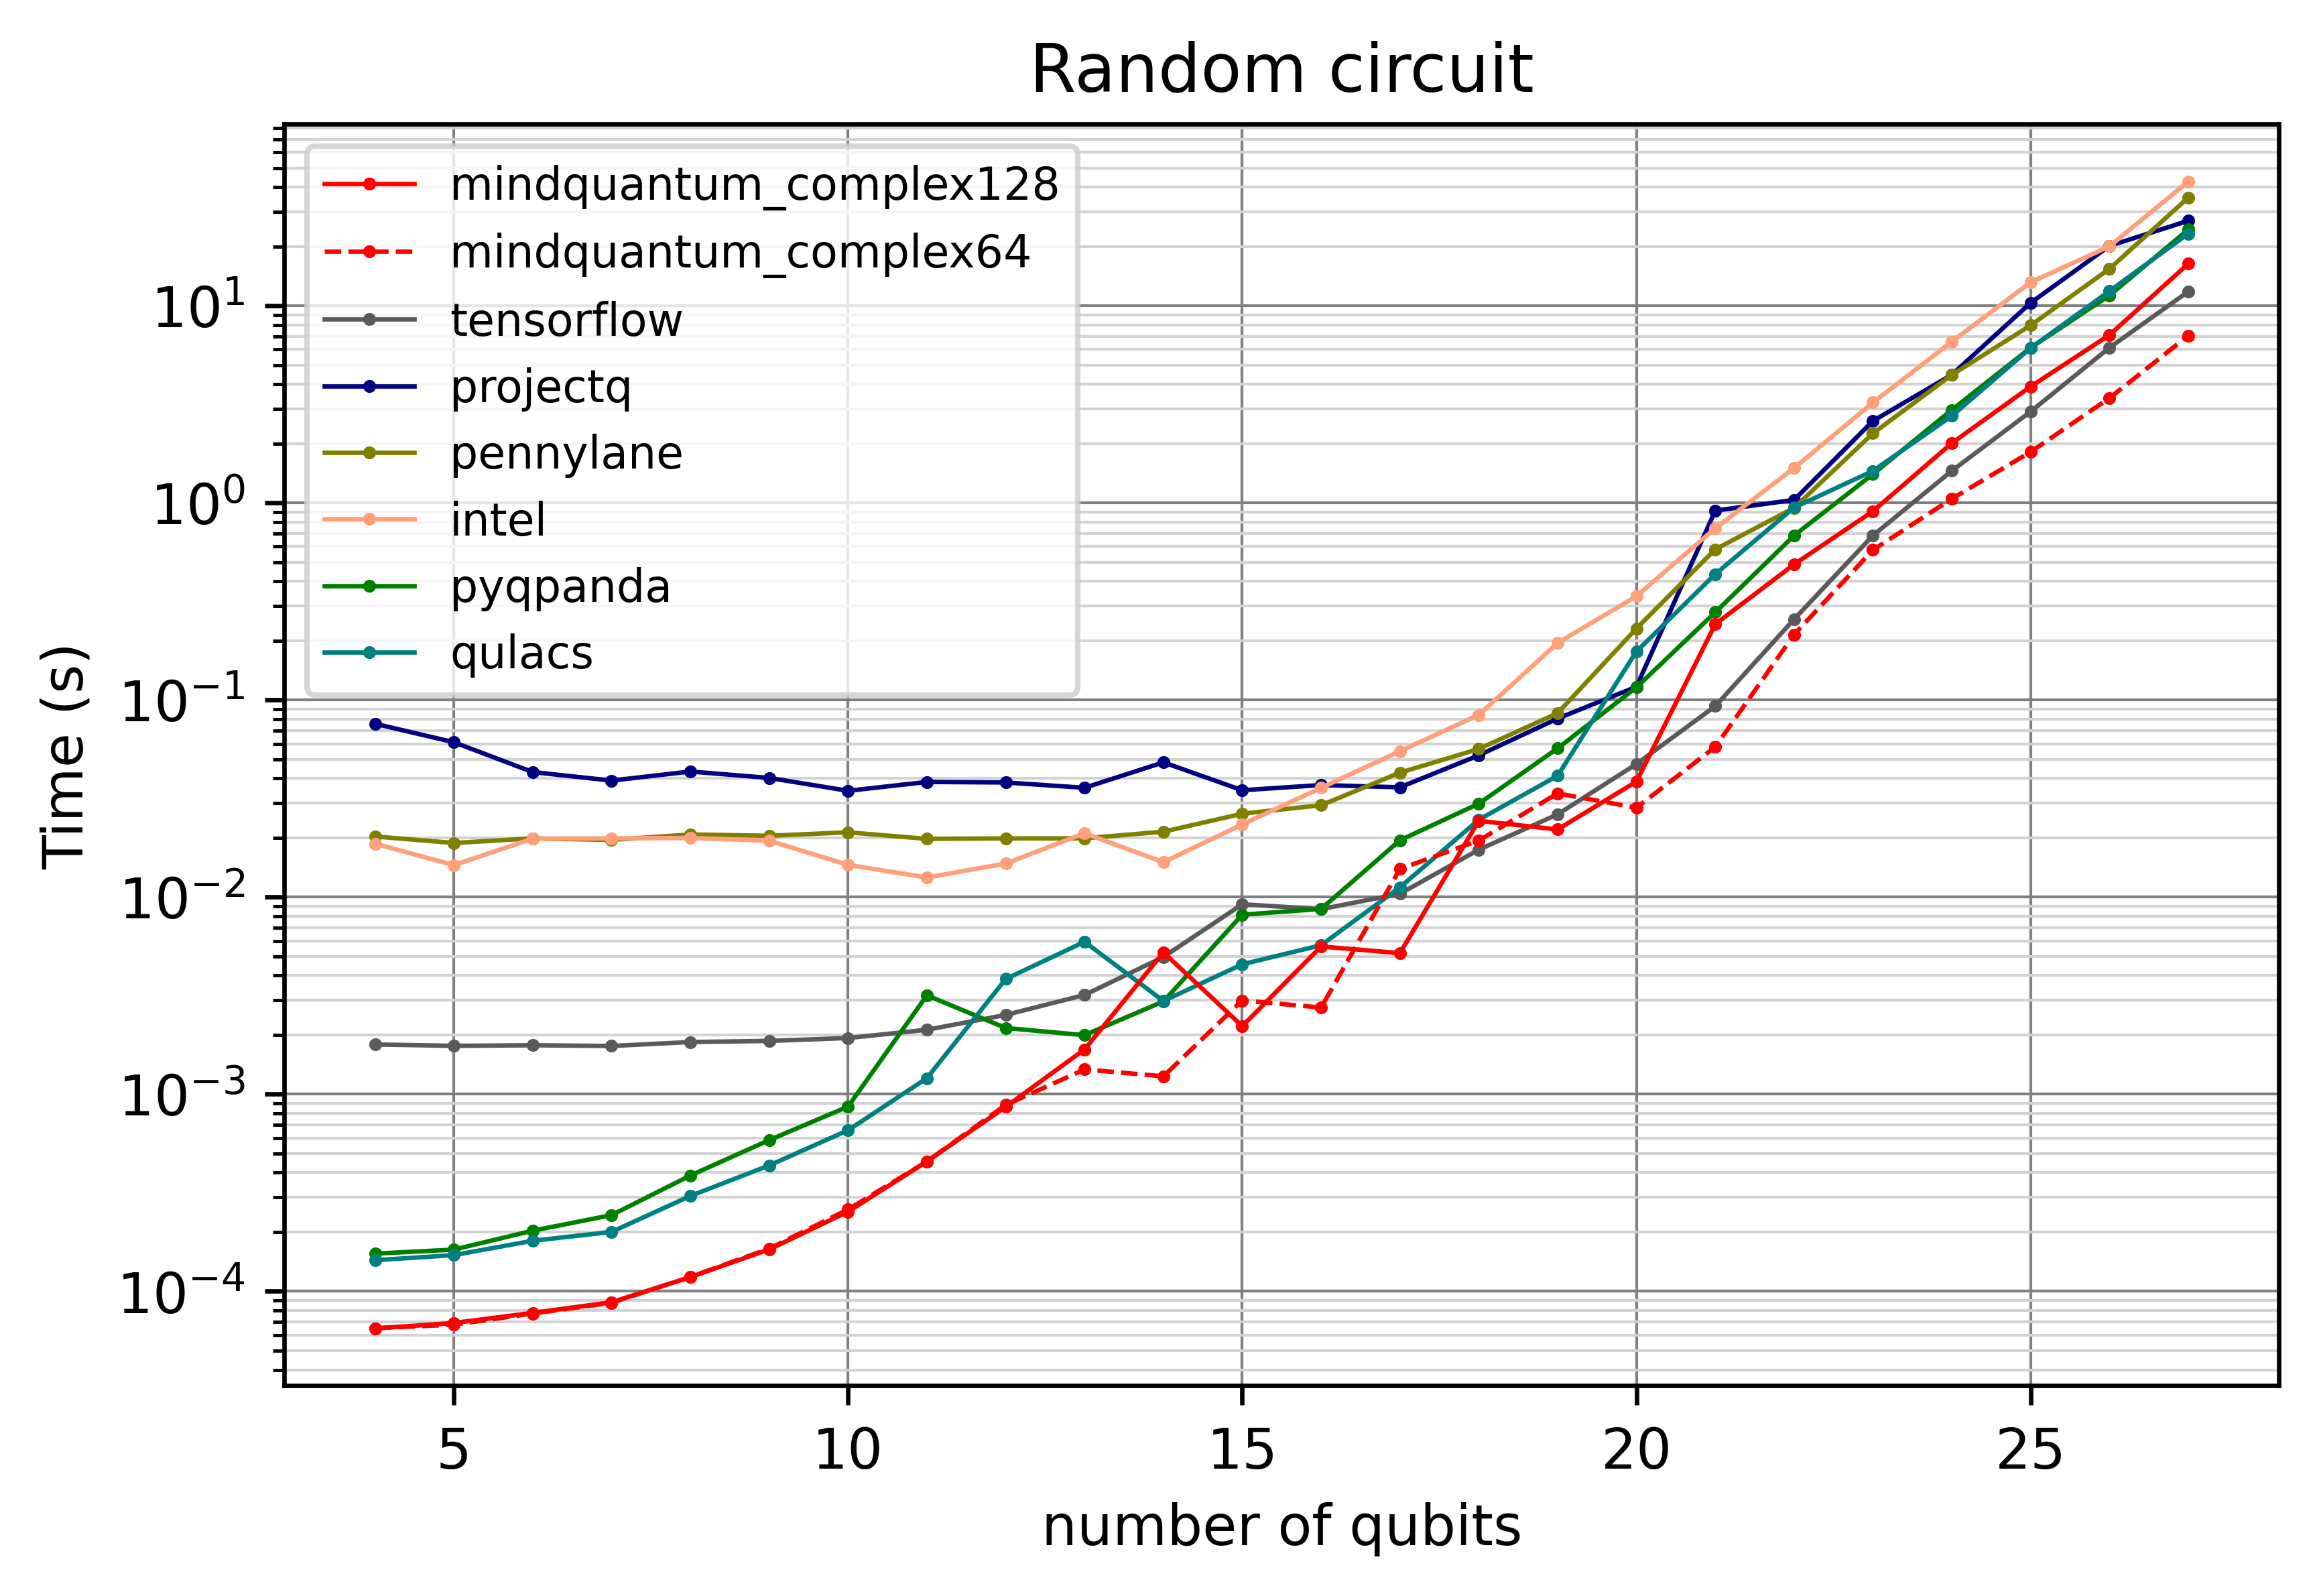
\includegraphics[width=\textwidth]{images/7_Random_circuit_CPU.png}
        \caption{CPU 后端上的随机线路基准测试。}
        \label{7_random_circ_cpu}
    \end{subfigure}
    \begin{subfigure}{0.45\textwidth}
        \centering
        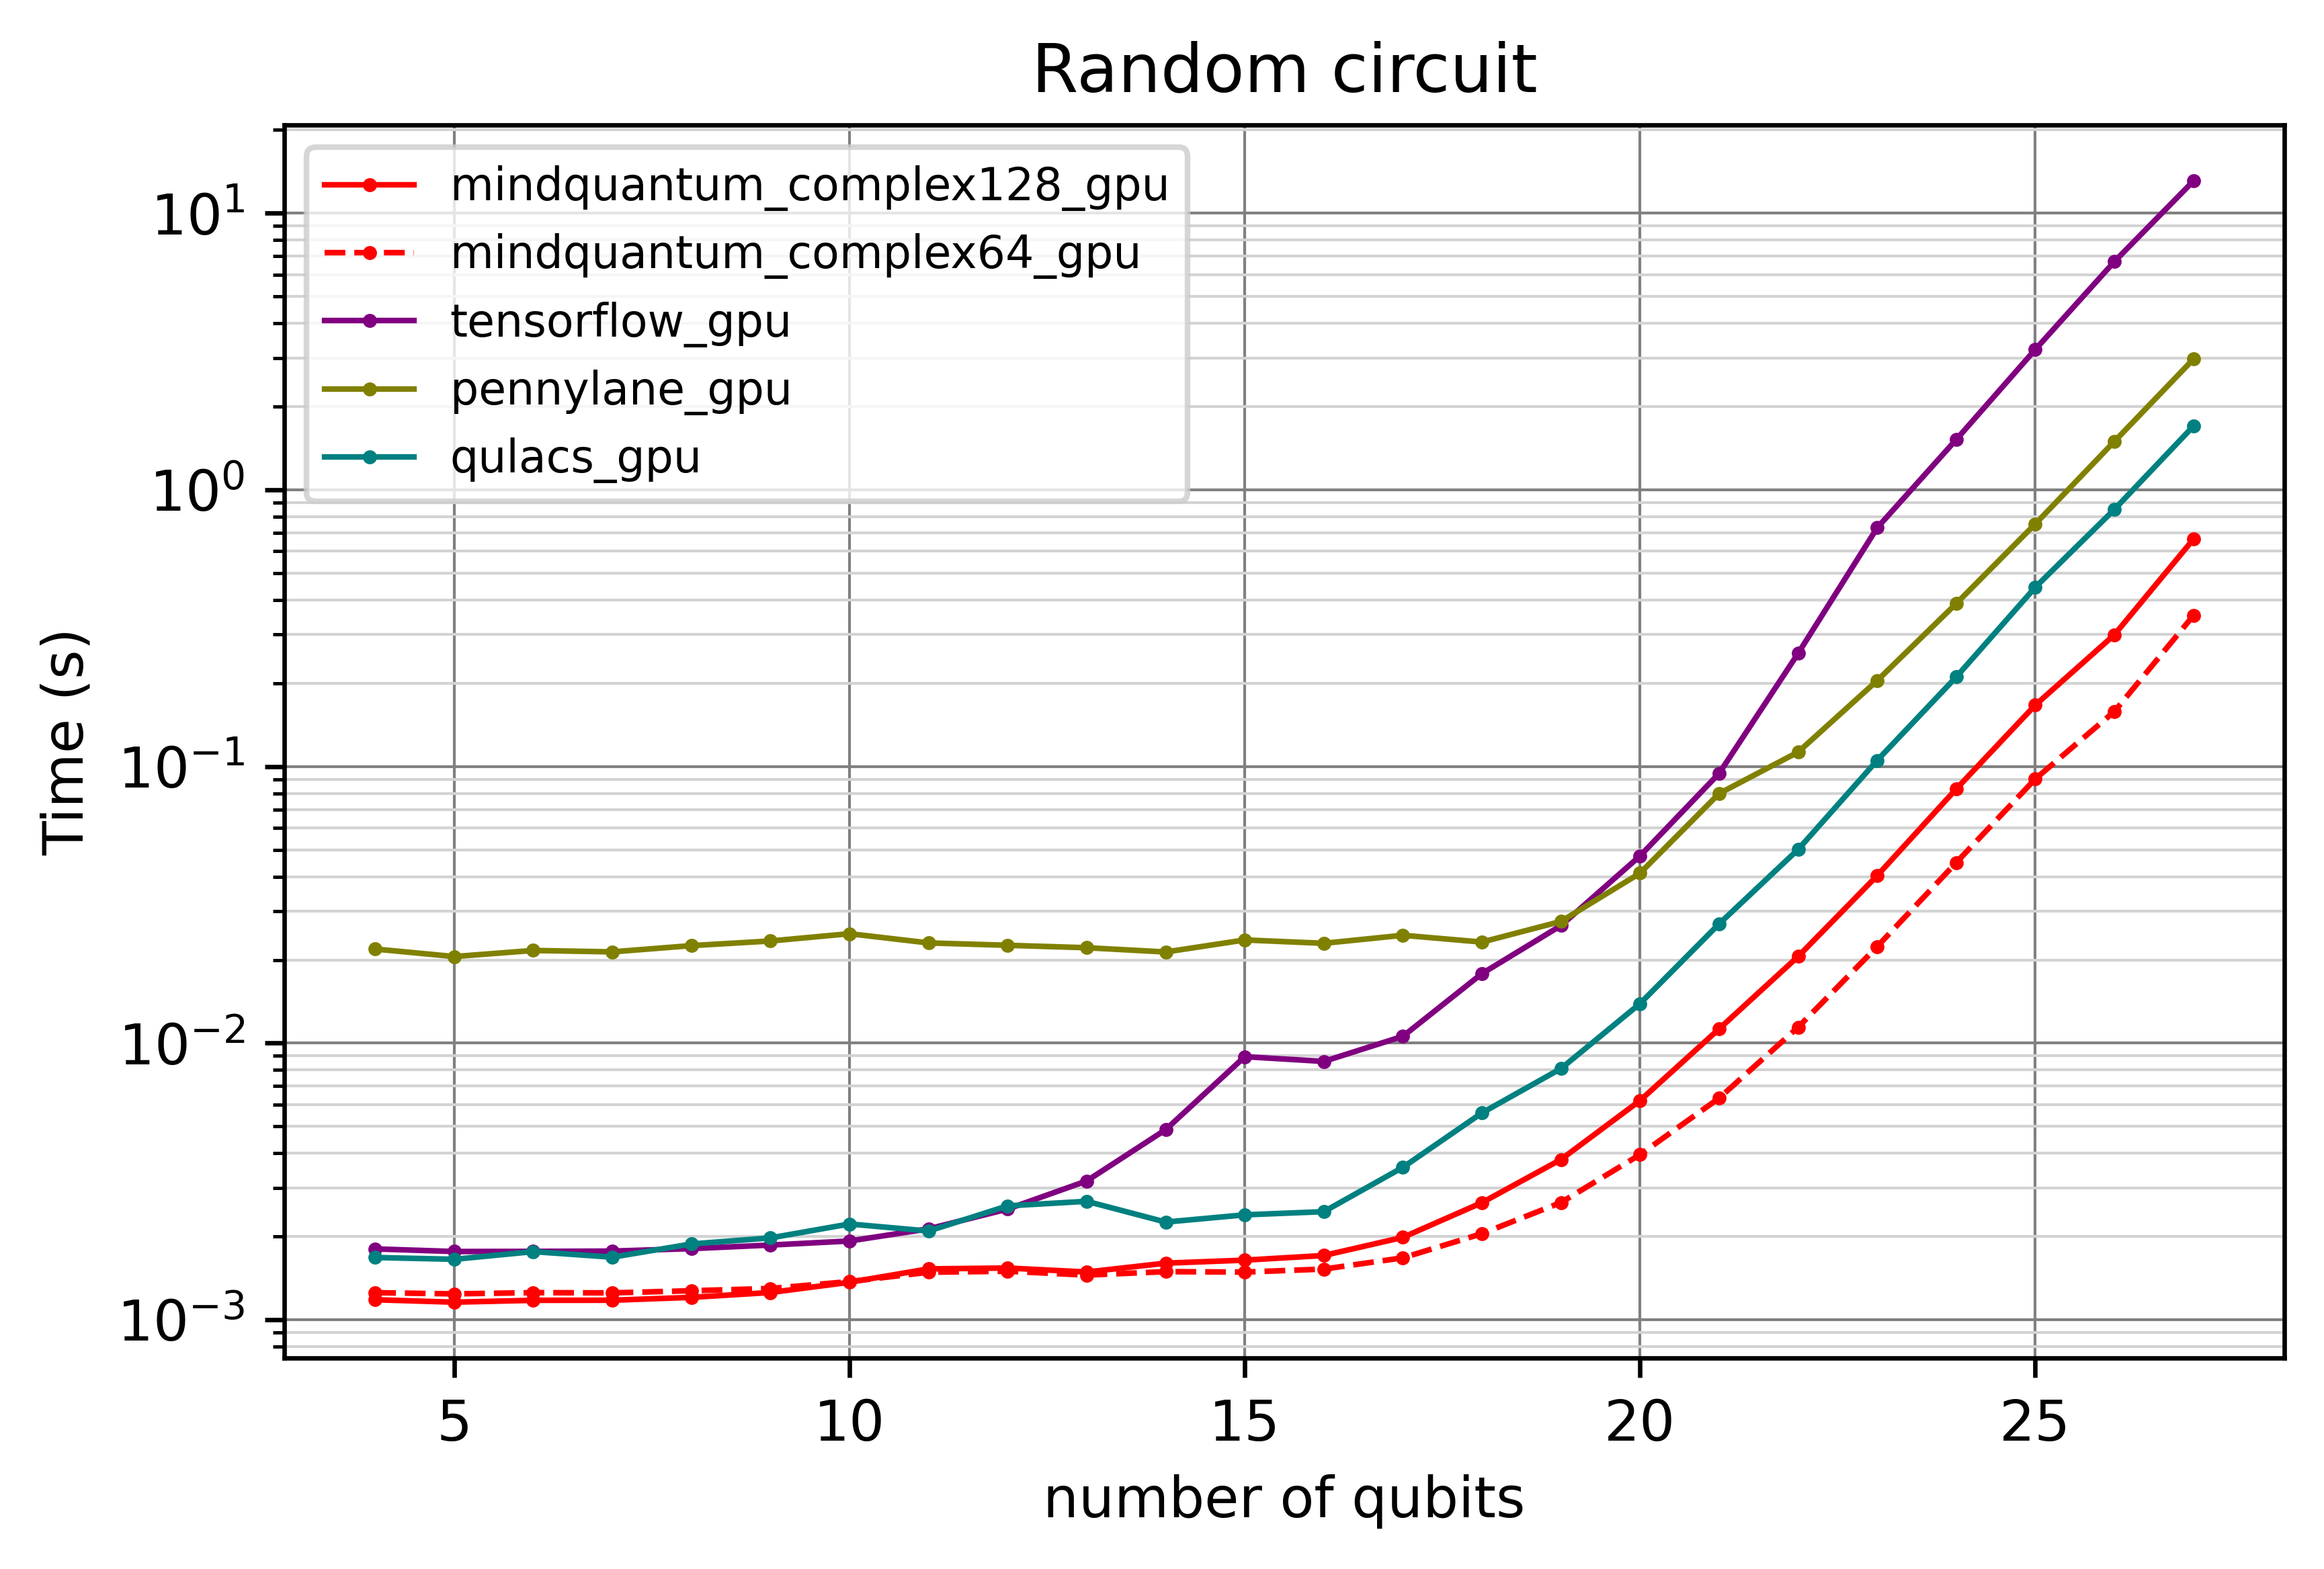
\includegraphics[width=\textwidth]{images/7_Random_circuit_GPU.png}
        \caption{GPU 后端上的随机线路基准测试。}
        \label{7_random_circ_gpu}
    \end{subfigure}
    \begin{subfigure}{0.45\textwidth}
        \centering
        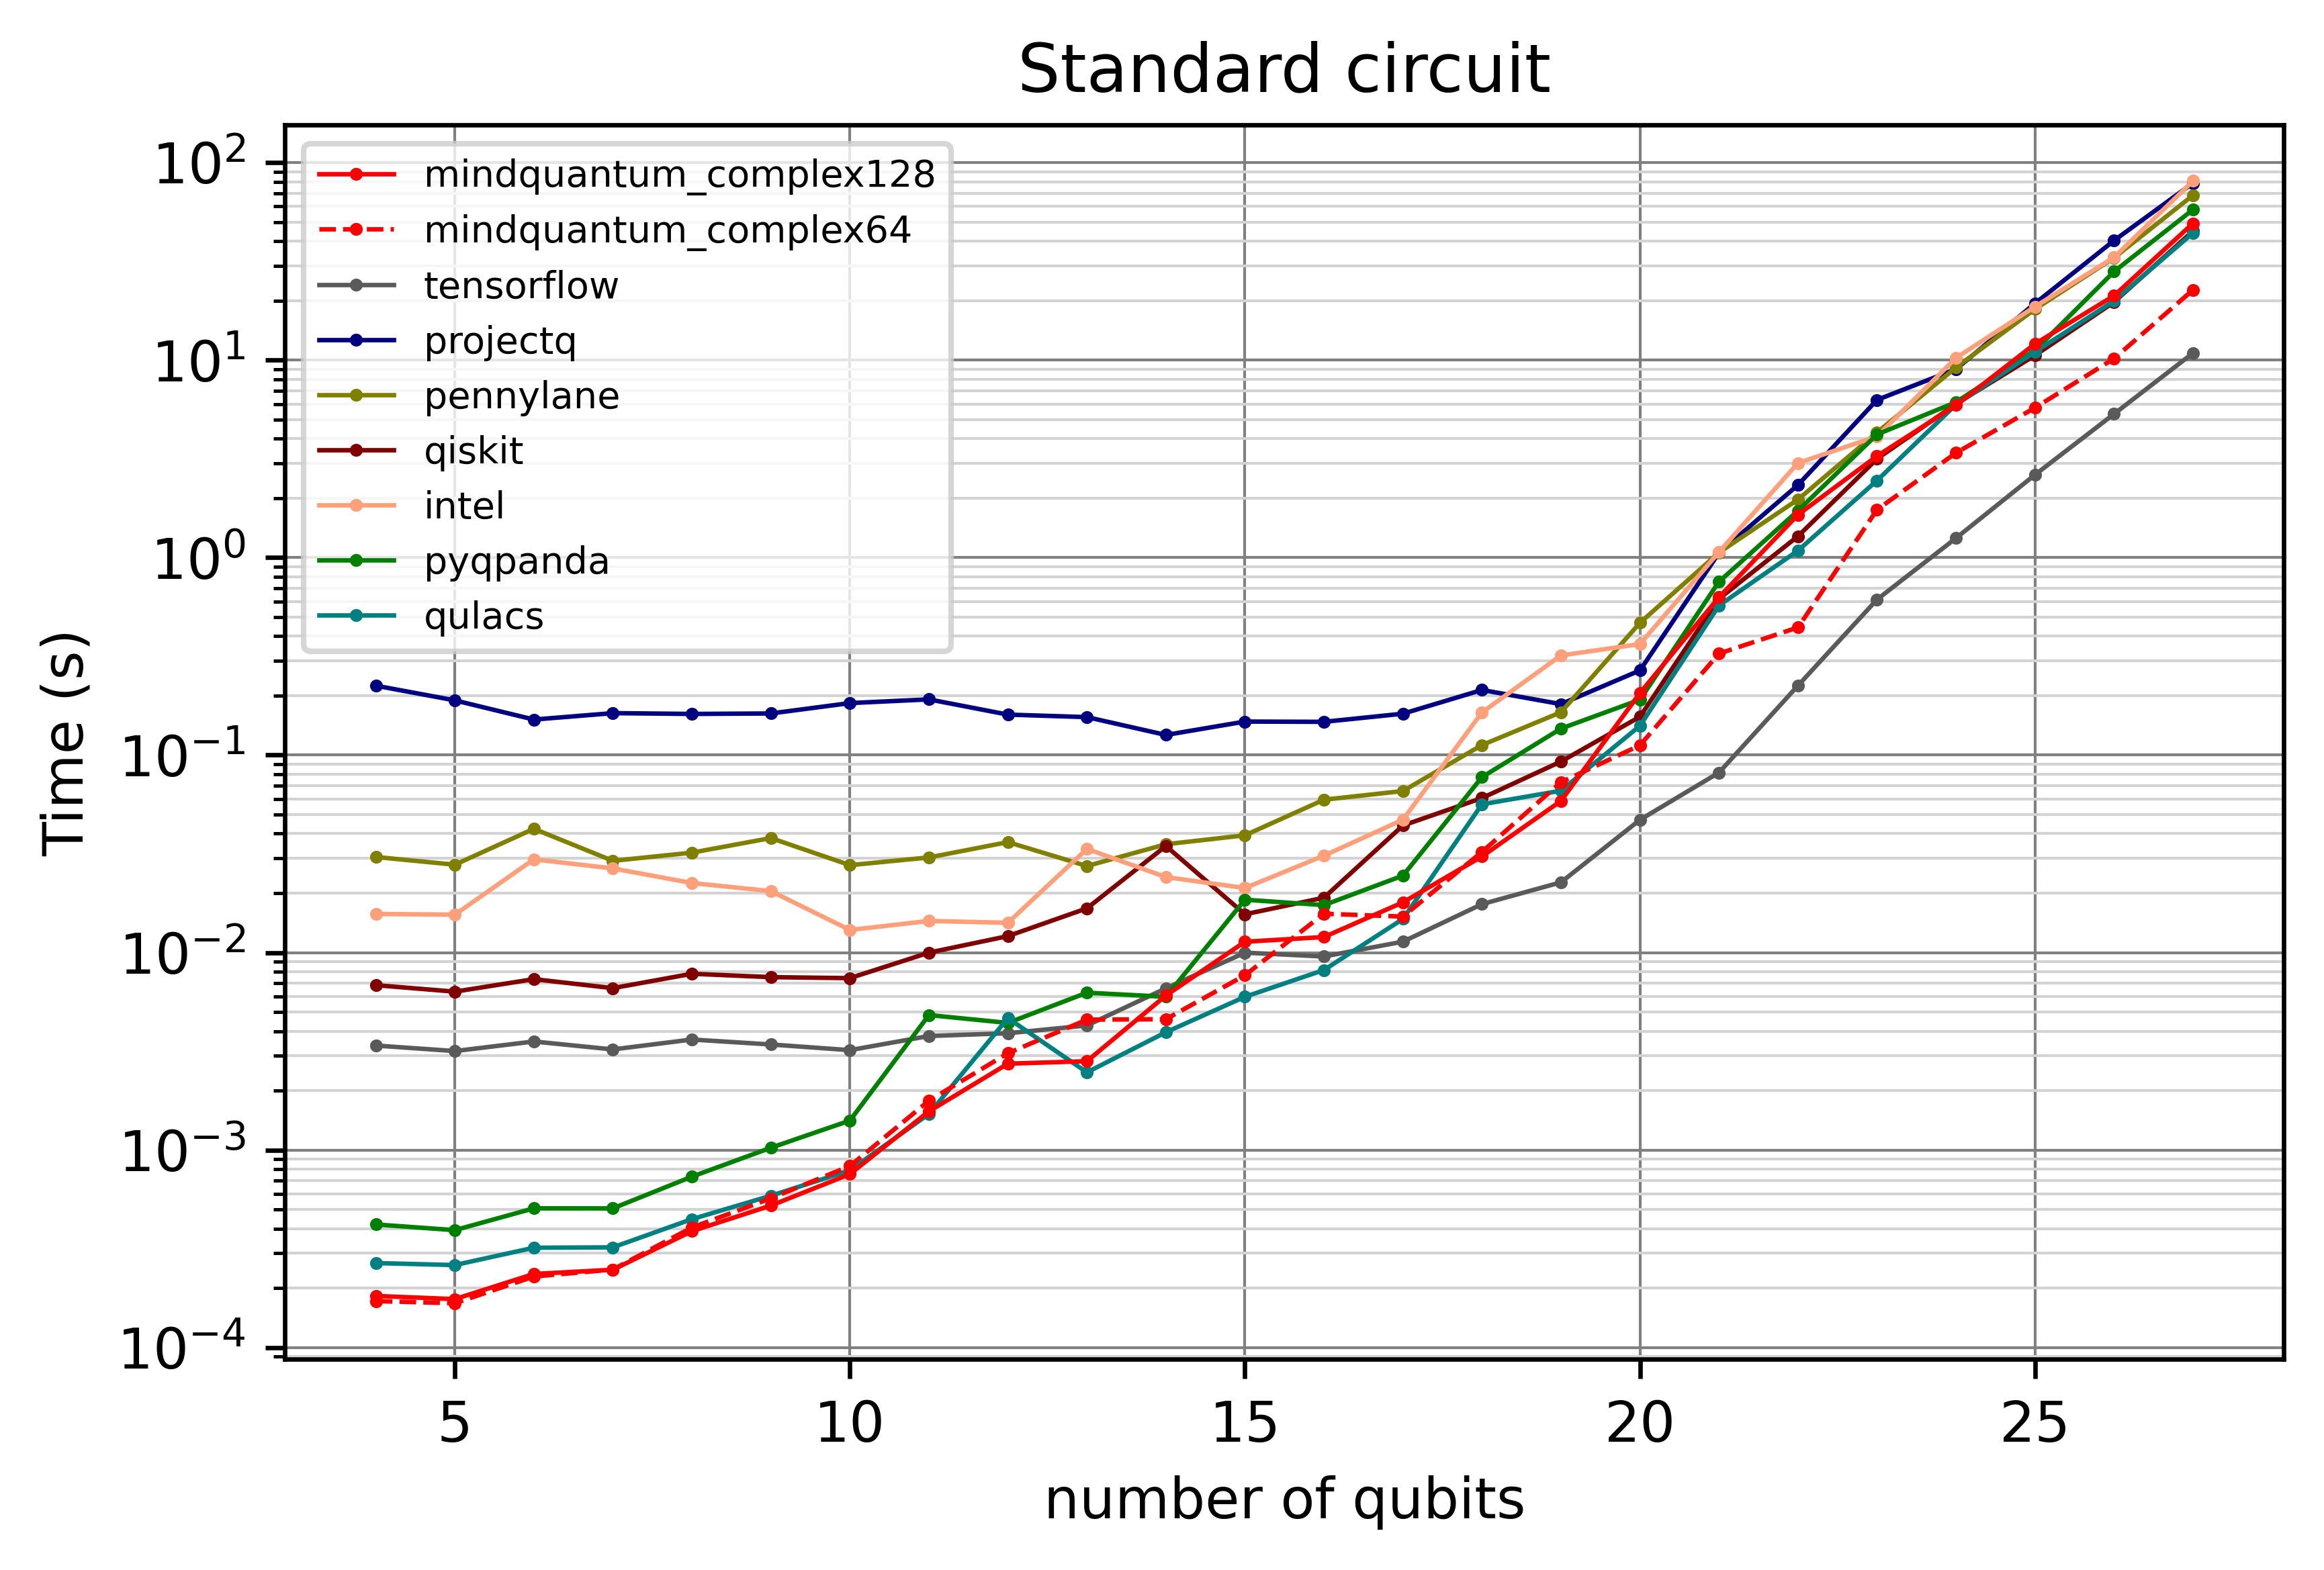
\includegraphics[width=\textwidth]{images/7_Simple_circuit_CPU.png}
        \caption{CPU 后端上的标准线路基准测试。}
        \label{7_simple_circ_cpu}
    \end{subfigure}
    \begin{subfigure}{0.45\textwidth}
        \centering
        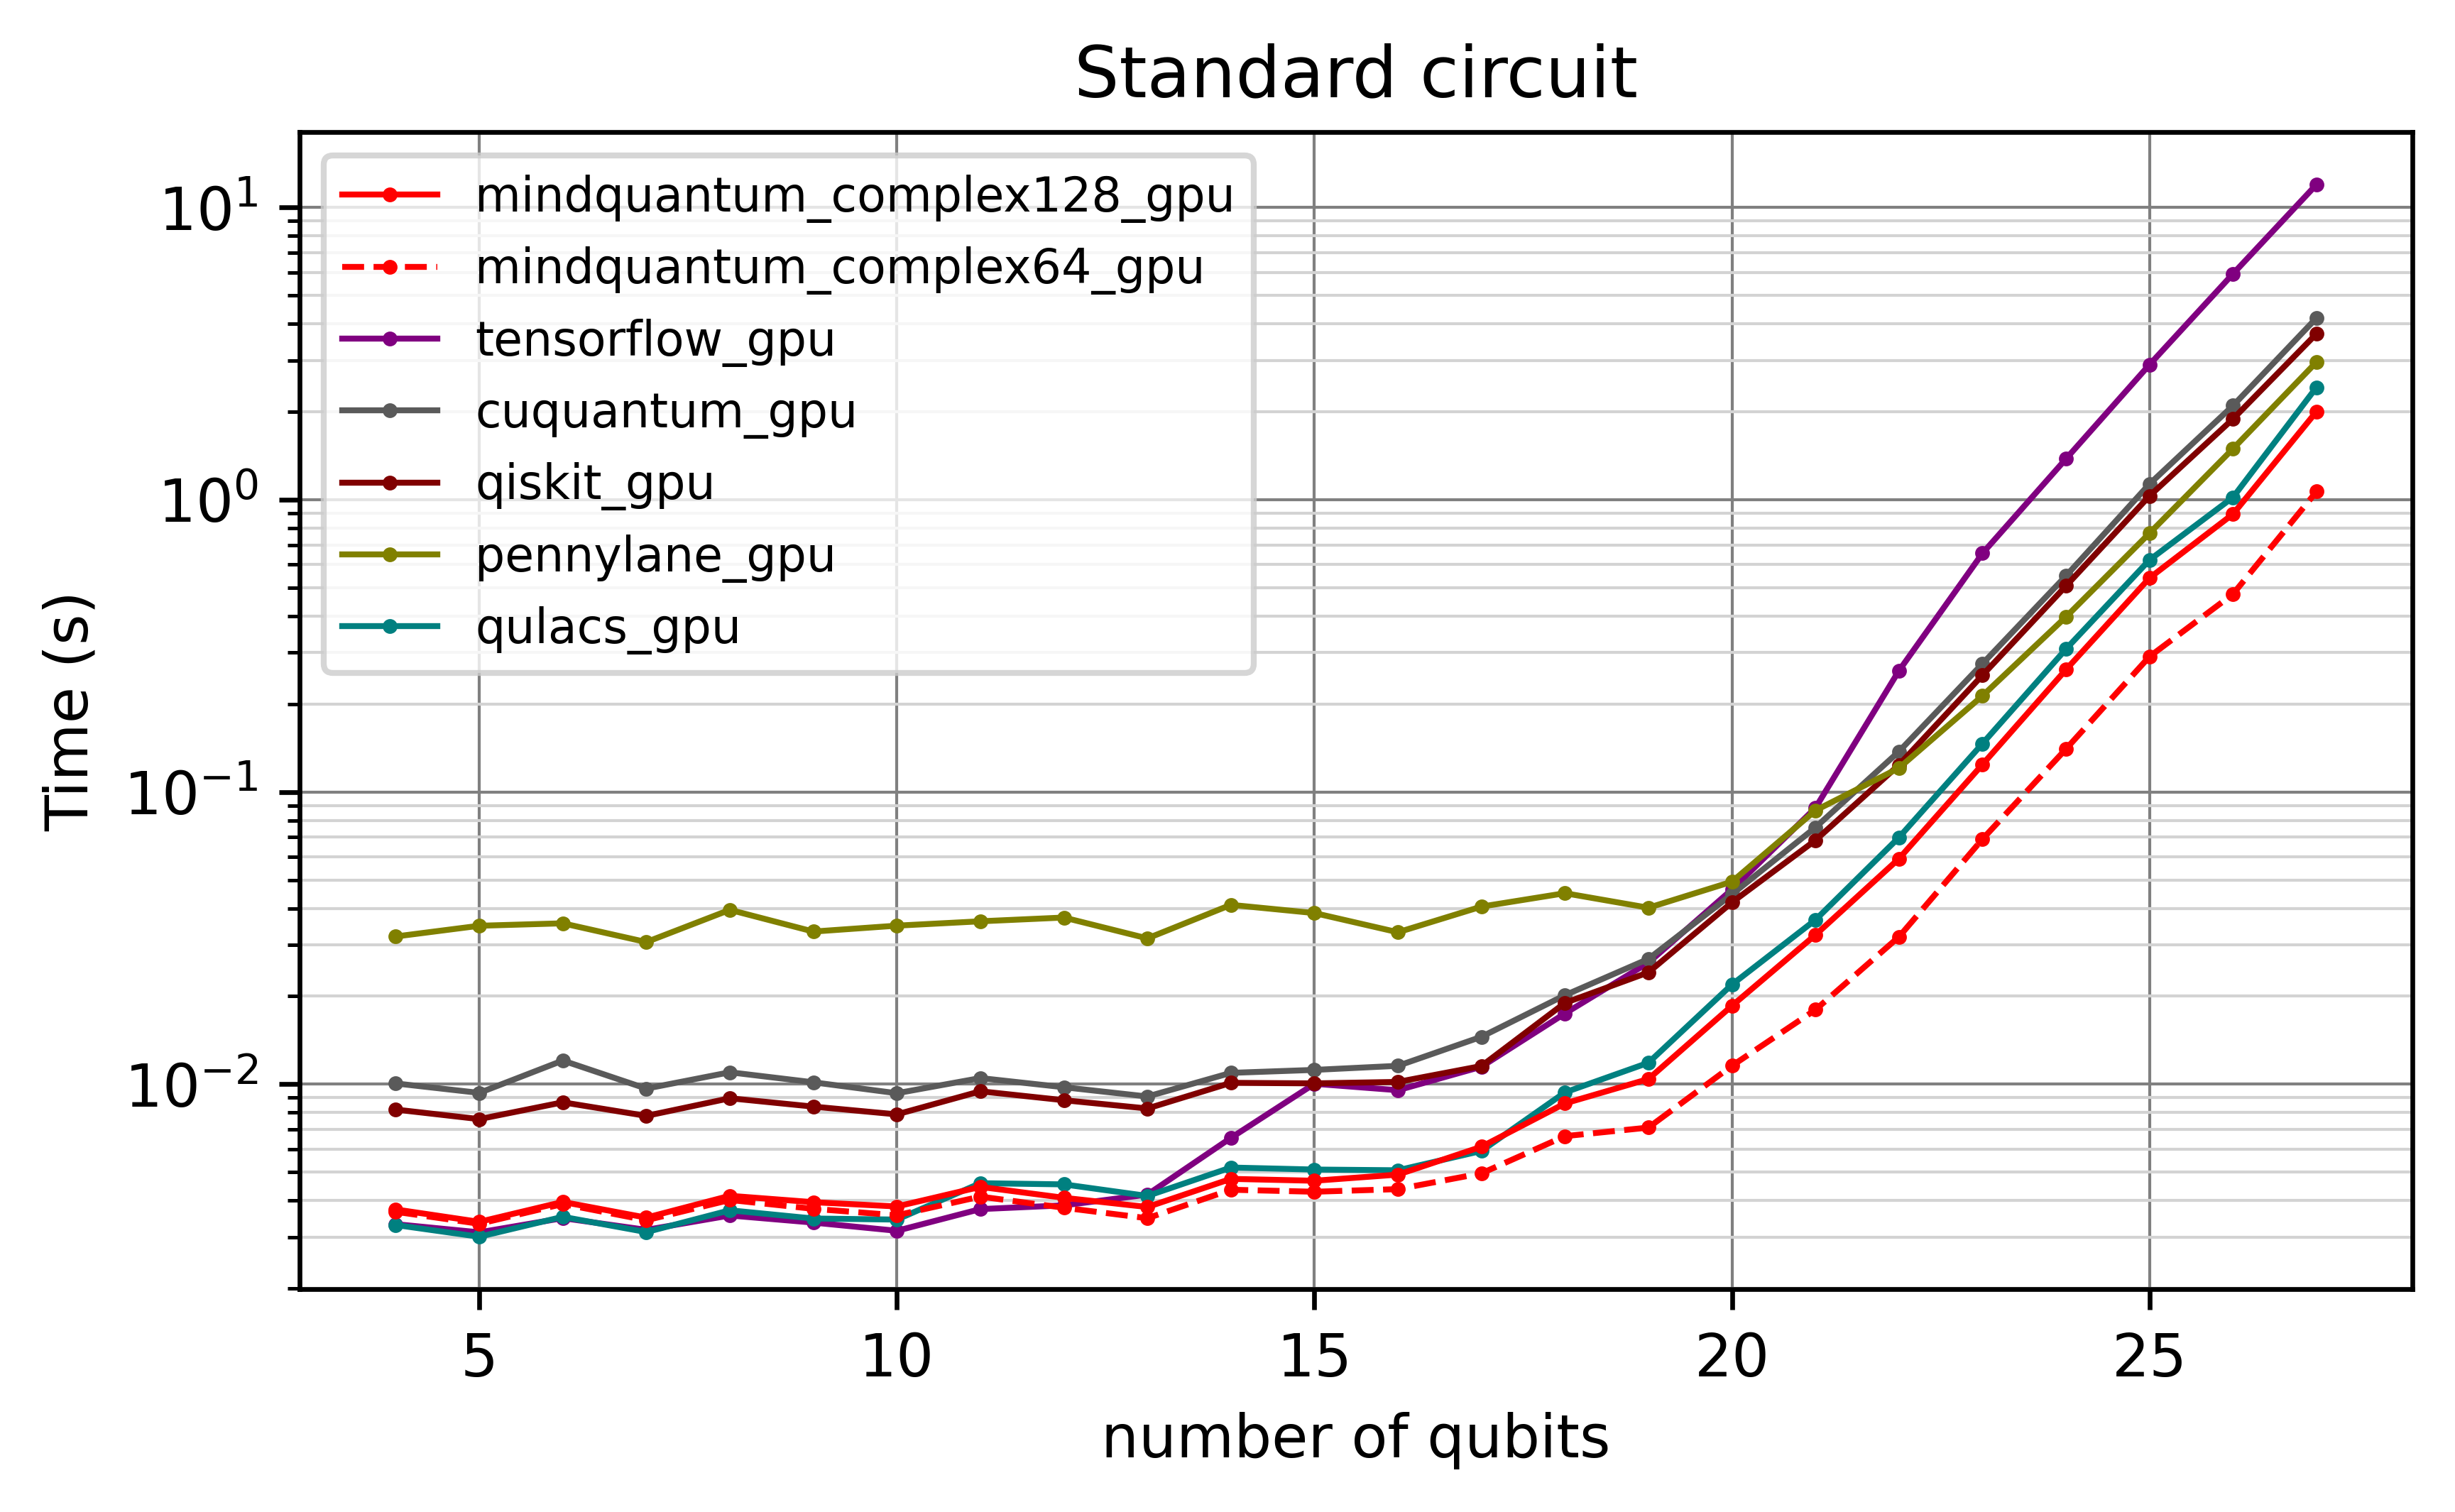
\includegraphics[width=\textwidth]{images/7_Simple_circuit_GPU.png}
        \caption{GPU 后端上的标准线路基准测试。}
        \label{7_simple_circ_gpu}
    \end{subfigure}
    \caption{不同后端上随机复杂线路与随机简单线路的基准测试。}
    \label{fig:benchmark_circ}
\end{figure*}

\subsection{运行随机线路任务}

在随机线路基准测试中，我们选择两类不同线路。第一类任务是复杂随机线路，量子比特数从 4 到 27 不等。复杂随机线路包含 X、Y、Z、H、CNOT、S、T、RX、RY、RZ、Rxx、Ryy、Rzz、SWAP 门及其受控版本。第二类任务是由对应复杂随机线路分解得到的简单随机线路，其中仅包含基础门集合。除 TensorFlow Quantum 外，基准测试中各模拟器均采用双精度。基准测试结果如图 \ref{fig:benchmark_circ} 所示。


总体而言，模拟时间会随线路规模呈指数增长。然而，当量子比特数较小时，\MindQuantum、Qulacs 和 Qpanda 在耗时方面相较其他框架具有明显优势，这主要来自 API 调用开销的差异。值得注意的是，在 13 量子比特位置附近出现了轻微下降，这是因为 \MindQuantum\ 以 13 个量子比特作为阈值；当量子比特数大于 13 时，会启用 OpenMP 进行多线程并行计算，否则使用单线程模拟。这样设计的原因是，当量子比特数较小时，多线程计算反而会降低运行速度。随着线路规模继续增大，\MindQuantum\ 和 Qulacs 保持了良好的速度优势，可以判断这两个框架在底层实现上已经优化到接近极限。在处理大比特数简单线路时，TensorFlow Quantum 表现出优势，原因有两点：第一，它采用单精度计算；第二，它针对基础量子门加入了更多专门优化。

\begin{figure*}
    \centering
    \begin{subfigure}{0.9\textwidth}
        \centering
        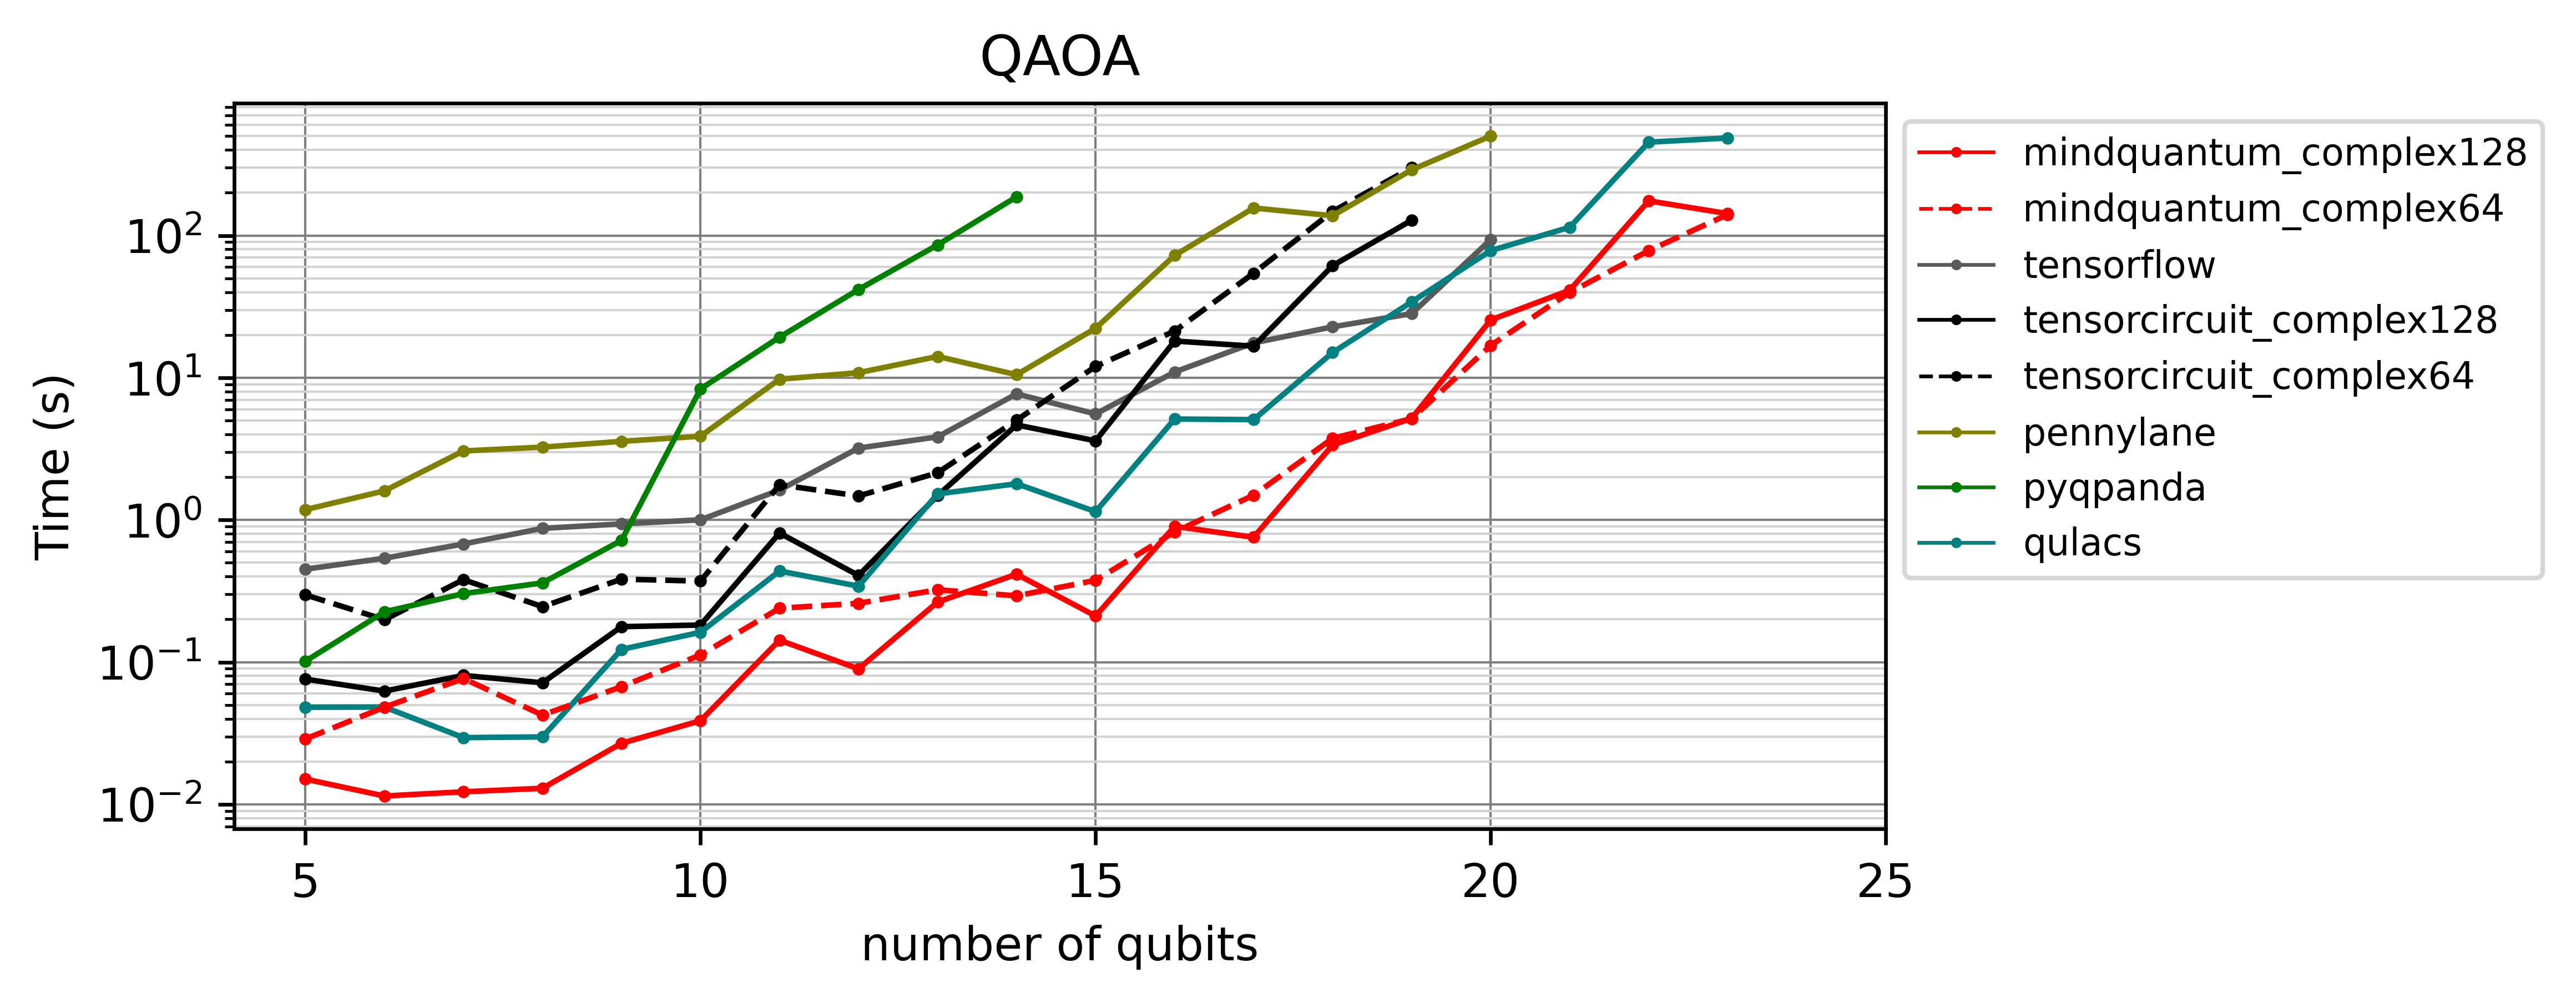
\includegraphics[width=\textwidth]{images/7_QAOA_CPU.png}
        \caption{CPU 上 4-正则图 QAOA 端到端优化基准测试。}
        \label{7_regular_4_cpu}
    \end{subfigure}
    \begin{subfigure}{0.9\textwidth}
        \centering
        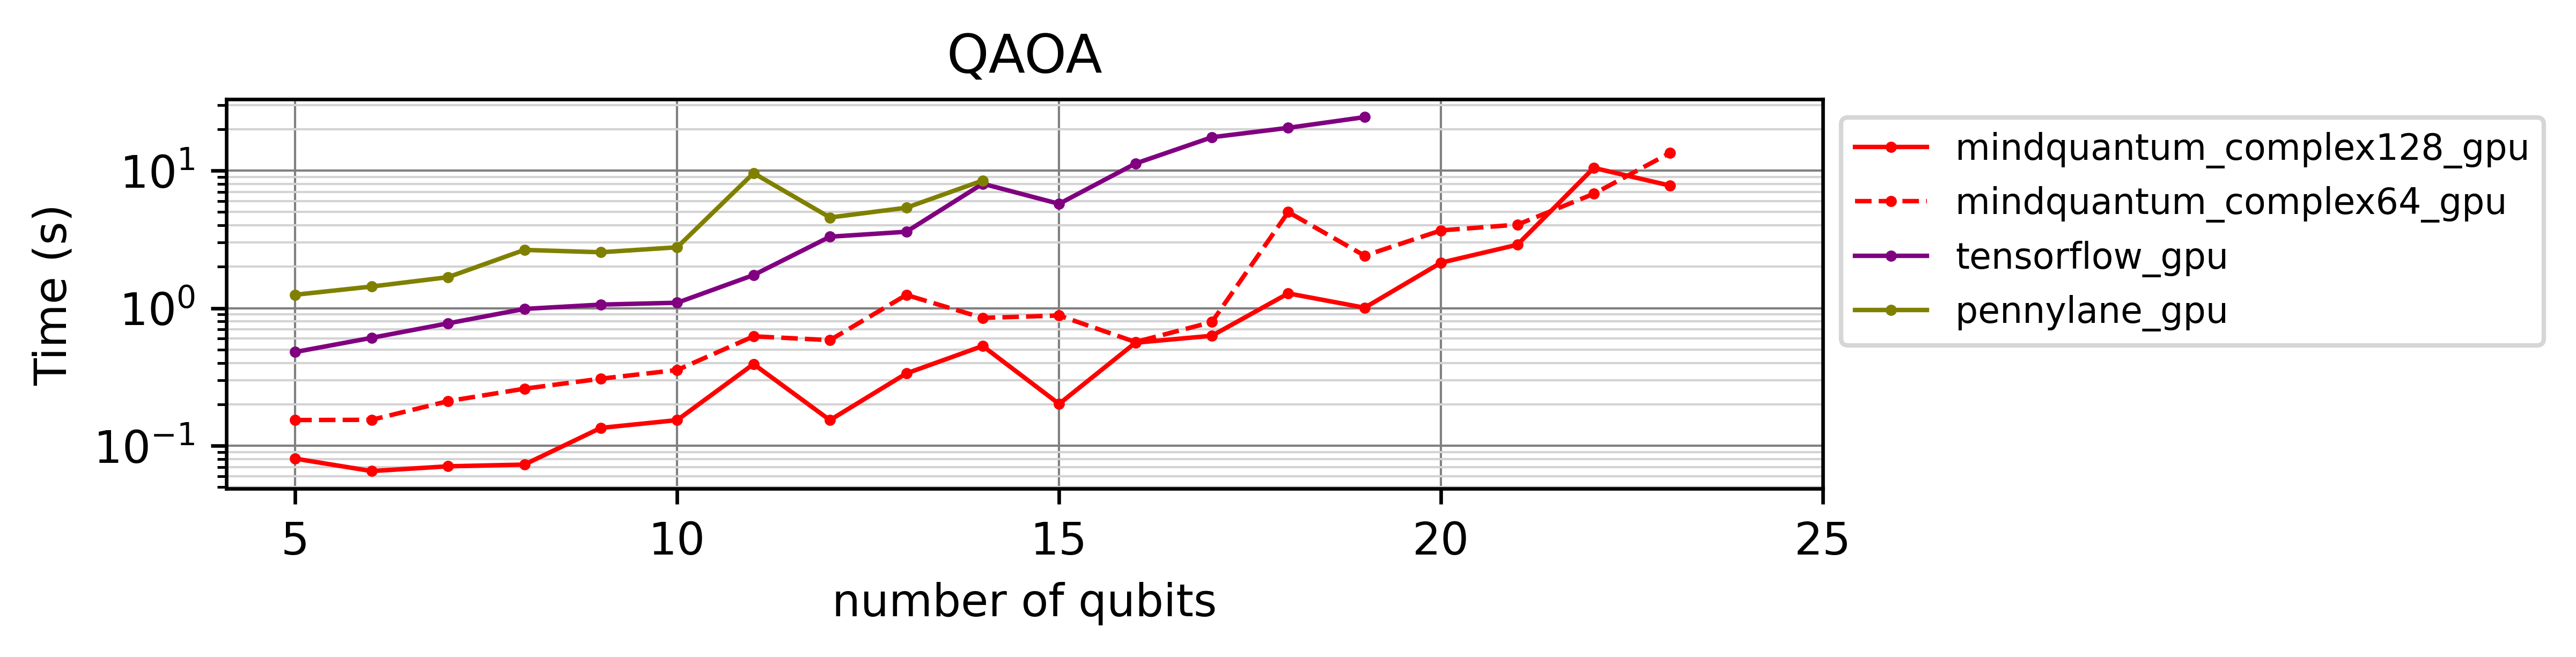
\includegraphics[width=\textwidth]{images/7_QAOA_GPU.png}
        \caption{GPU 上 4-正则图 QAOA 端到端优化基准测试。}
        \label{7_regular_4_gpu}
    \end{subfigure}
    \caption{不同后端上的 QAOA 基准测试。}
    \label{fig:benchmark_qaoa}
\end{figure*}

\subsection{QAOA 任务}

变分量子算法也是 NISQ 阶段非常重要的一类算法。在本部分中，我们选择量子近似优化算法进行基准测试，以进一步展示框架在求解实际问题时的性能。我们使用 QAOA 求解 4-正则图的最大割问题，问题规模从 5 个节点到 23 个节点不等。ansatz 线路通过一步 Trotter 分解得到。优化器采用 \code{scipy.optimize.minimize()} 中的 BFGS 方法。由于大规模 QAOA 任务耗时较长，当某个框架的运行时间达到指定阈值时，我们会停止其执行。因此，在结果图中，各框架数据点所能达到的最大量子比特数并不一致。基准测试结果如图 \ref{fig:benchmark_qaoa} 所示。

总体来看，随着问题规模增加，所有框架的求解时间都呈指数增长。然而，对于这些问题，\MindQuantum\ 相比其他框架至少快一个数量级。这主要得益于 MindQuantum 中针对参数化量子线路梯度计算优化过的伴随方法，以及高效的线路演化实现。



\section{在量子芯片上执行}
\label{sec:chip}
\subsection{量子线路编译与优化}
在 \Simulator\ 上模拟量子线路时，通常不需要考虑该量子线路是否真的能在量子芯片上执行；我们的关注点仅在于研究算法本身的可行性。然而，当考虑真实量子芯片时，芯片上可执行的量子门集合是有限的。此外，由于量子噪声的存在，我们也希望尽可能降低量子线路深度。因此，需要对量子线路进行编译和优化。本节将说明 \MindQuantum\ 如何完成量子线路的编译与优化。

这里，我们使用 DAG（Directed Acyclic Graph，有向无环图）作为量子线路编译工具。如图 \ref{fig:compiler} 所示，量子线路会被转换为 DAG。基于该 DAG，可以应用 \MindQuantum\ 中内置的编译规则，例如 \BasicDecompose、\FullyNeighborCanceler 和 \GateReplacer，以完成量子编译和优化。此外，我们还提供了两个稳健的管理器来组织这些编译规则，分别是 \SequentialCompiler 和 \KroneckerSeqCompiler。\SequentialCompiler 中的规则会按顺序各执行一次，而 \KroneckerSeqCompiler 中的规则会持续执行，直到无法进一步编译为止。

\begin{figure}
    \centering
    \begin{subfigure}{0.25\textwidth}
        \centering
        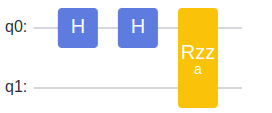
\includegraphics[width=\textwidth]{images/8_1_ori_circ.png}
        \caption{原始量子线路。}
        \label{fig:compiler_a}
    \end{subfigure}
    \begin{subfigure}{0.3\textwidth}
        \centering
        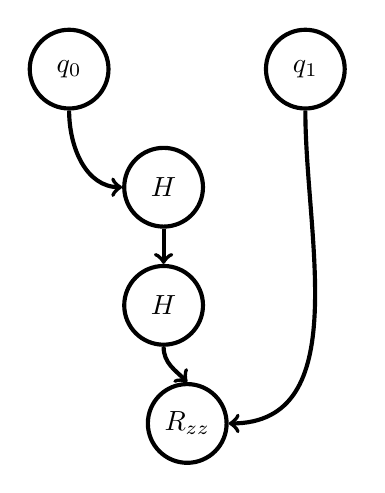
\begin{tikzpicture}[
                transparent/.style={circle, draw=black, fill=none, font=\sffamily, text centered, line width=1.5pt, minimum size=1cm}
            ]
            \node (q0) at (0, 0) [transparent] {$q_0$};
            \node (q1) at (3, 0) [transparent] {$q_1$};
            \node (H1) at (1.2, -1.5) [transparent] {$H$};
            \node (H2) at (1.2, -3) [transparent] {$H$};
            \node (Rzz) at (1.5, -4.5) [transparent] {$R_\text{zz}$};
            \draw [->, line width=1.5pt] (q0.south) to[out=270, in=180] (H1.west);
            \draw [->, line width=1.5pt] (H1.south) to[out=270, in=90] (H2.north);
            \draw [->, line width=1.5pt] (H2.south) to[out=270, in=135] (Rzz.north);
            \draw [->, line width=1.5pt] (q1.south) to[out=270, in=0] (Rzz.east);
        \end{tikzpicture}
        \caption{量子线路的 DAG 表示。}
    \end{subfigure}
    \begin{subfigure}{0.45\textwidth}
        \centering
        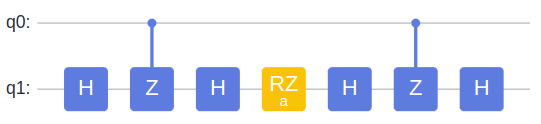
\includegraphics[width=\textwidth]{images/8_1_compiled_circ.png}
        \caption{编译和优化后的线路。}
        \label{fig:compiler_c}
    \end{subfigure}
    \caption{将量子线路转换为 DAG，并依据给定编译规则完成编译。}
    \label{fig:compiler}
\end{figure}

作为示例，我们将使用不同规则来编译并优化图 \ref{fig:compiler_a} 中的线路。首先，使用 \BasicDecompose 和 \FullyNeighborCanceler 构建一个 \KroneckerSeqCompiler，以便将 $R_\text{zz}$ 门分解为基础量子门，并抵消两个 Hadamard 门。接下来，假设芯片只能执行 CZ 门，则将 CNOT 门替换为 CZ 门。
\begin{lstlisting}
from mindquantum.core.circuit import Circuit
from mindquantum.algorithm.compiler import *

circ = Circuit().h(0).h(0).rzz('a', [0, 1])

compiler = SequentialCompiler([
    KroneckerSeqCompiler([
        BasicDecompose(),
        FullyNeighborCanceler()
    ]),
    CXToCZ()
])

new_circ = compile_circuit(compiler, circ)
\end{lstlisting}


\subsection{量子比特映射}

受量子硬件实现中的若干物理限制影响，当前量子计算机通常被归类为含噪中等规模量子（Noisy Intermediate-Scale Quantum, NISQ）硬件。NISQ 硬件的典型特征是量子比特数量有限（约 50 到数百个）且操作含噪。此外，当前超导量子芯片的实现并不具备理想的量子比特全连接结构，而通常至多支持近邻连接。由于这些约束，大多数量子算法无法直接在 NISQ 设备上执行。为了实现算法中的双量子比特门，需要将逻辑量子比特动态重映射到物理量子比特上。这一问题称为量子比特映射问题 \cite{10323857}。

量子比特映射问题已被证明是 NP-Complete 问题 \cite{siraichi2018qubit}。考虑到时间复杂度，\MindQuantum\ 选择了一种基于 SWAP 的双向启发式算法，名为 SABRE \cite{li2019tackling}。

图 \ref{fig:qubit-mapping-sample} 给出了一个量子比特映射示例。
物理硬件有自身的物理连接图。当我们将逻辑量子比特映射到物理量子比特上时，由于两个量子比特在物理连接图中可能并不相连，某些双量子比特门可能无法直接实现。最直接的解决方案是使用 SWAP 门。通过若干 SWAP 操作，即可实现逻辑线路。

\begin{figure}
	\centering
	\begin{subfigure}{0.1\textwidth}
		\centering
		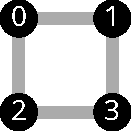
\includegraphics[width=\textwidth]{8.2_figures/example_topo}
		\caption{物理拓扑图。}
	\end{subfigure}
	\begin{subfigure}{0.3\textwidth}
		\centering
		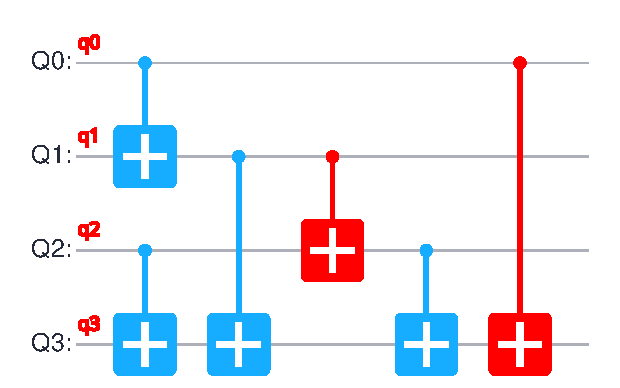
\includegraphics[width=0.9\textwidth]{8.2_figures/example_original}
		\caption{逻辑线路。}
	\end{subfigure}

	\begin{subfigure}{0.45\textwidth}
		\centering
		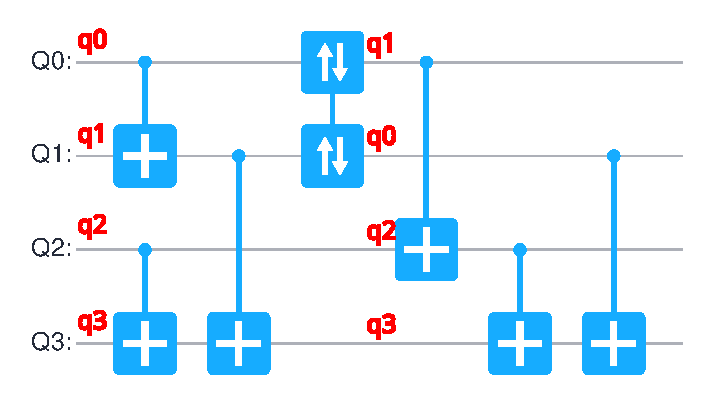
\includegraphics[width=\textwidth]{8.2_figures/example_updated}
		\caption{修正后的线路。}
	\end{subfigure}

	\caption{量子比特映射示例。}
	\label{fig:qubit-mapping-sample}
\end{figure}

该算法的目标是减少 SWAP 门数量和线路深度。

首先，可以生成一个有向无环图（DAG）来表示给定量子线路中双量子比特门之间的约束关系。单量子比特门总是可以执行，因此无需考虑。可以将每个双量子比特门标记为 $g_i(q_j, q_k)$，表示 $g_i$ 作用在 $q_j$ 和 $q_k$ 上。如果 $g_x(q_i, q_j)$ 后面跟着 $g_y(q_j, q_k)$，则向 DAG 中加入一条边 $(g_x, g_y)$。图 \ref{fig:qubit-mapping-dag} 展示了一个 DAG 生成示例。

\begin{figure}
	\centering
	\begin{subfigure}{0.49\textwidth}
		\centering
		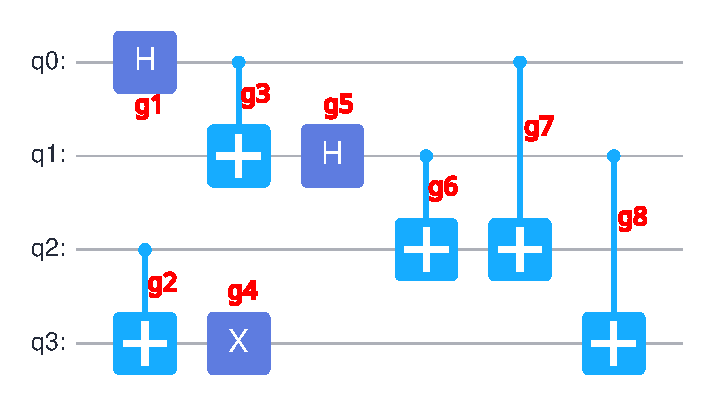
\includegraphics[width=\textwidth]{8.2_figures/dag_circuit}
		\caption{量子线路。}
	\end{subfigure}
	\begin{subfigure}{0.49\textwidth}
		\centering
		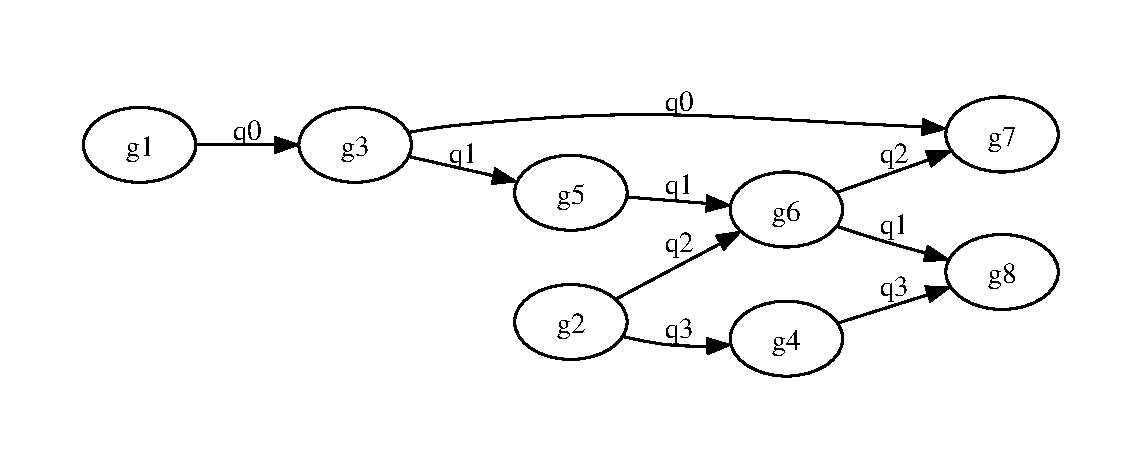
\includegraphics[width=\textwidth]{8.2_figures/dag_dag}
		\caption{生成的 DAG。}
	\end{subfigure}
	\caption{DAG 生成示例。}
	\label{fig:qubit-mapping-dag}
\end{figure}

该算法的核心思想十分直接。类似于拓扑排序，我们可以构造一个当前需要执行的前沿层。如果某个门在当前映射下可以执行，则执行该门并更新前沿层。当没有门可以执行时，计算可用的 SWAP。最后，选择启发式函数值最小的 SWAP。

基础启发式函数来自最近邻代价函数。对于两个物理量子比特 $Q_i$ 和 $Q_j$，$D[Q_i][Q_j]$ 表示二者在物理连接图中的最短距离。对于给定前沿层 $F$ 和当前映射 $\pi$，基础函数定义见式 \eqref{eq:qubit-mapping-h-basic}。
\begin{equation} \label{eq:qubit-mapping-h-basic}
	H_{\text{basic}} = \sum_{g \in F} D[\pi (g.q_1)][\pi (g.q_2)].
\end{equation}

$H_{\text{basic}}$ 只考虑前沿层。如果希望进行前瞻，可以加入一个扩展集合 $E$，其中包含来自 $F$ 的若干最近后继门。$E$ 的大小是灵活的，取决于所需的前瞻能力。同时，$F$ 中的门应具有比 $E$ 更高的优先级。因此，引入权重参数 $0 \leq W < 1$。

到目前为止，该启发式函数倾向于减少 SWAP 门数量。我们还希望降低线路深度，二者之间存在权衡。为此，为每个量子比特加入一个 $decay$ 参数。如果某个量子比特上已经执行了很多操作，则它会具有更大的 $decay$。借助 $decay$，算法会倾向于选择操作较少的量子比特，从而提高线路并行度。修正后的启发式函数见式 \eqref{eq:qubit-mapping-h}。
\begin{equation} \label{eq:qubit-mapping-h}
	\begin{aligned}
		H =    & \max \left( \rm{decay}(\rm{SWAP.q_1}), \rm{decay}(\rm{SWAP.q_2}) \right)                \\
		\times & \Big\lbrace \frac{1}{|F|} \sum_{g \in F} D[\pi(g.q_1)][\pi(g.q_2)]  \\
		+      & \frac{W}{|E|} \sum_{g \in E} D[\pi(g.q_1)][\pi(g.q_2)] \Big\rbrace.
	\end{aligned}
\end{equation}

最后，还需要处理初始映射问题。已有研究表明，初始映射会对最终结果产生巨大影响。这里我们采用文献 \cite{li2019tackling} 中介绍的方法。图 \ref{fig:qubit-mapping-initial-mapping} 展示了更新初始映射的过程。

\begin{figure}
	\centering
	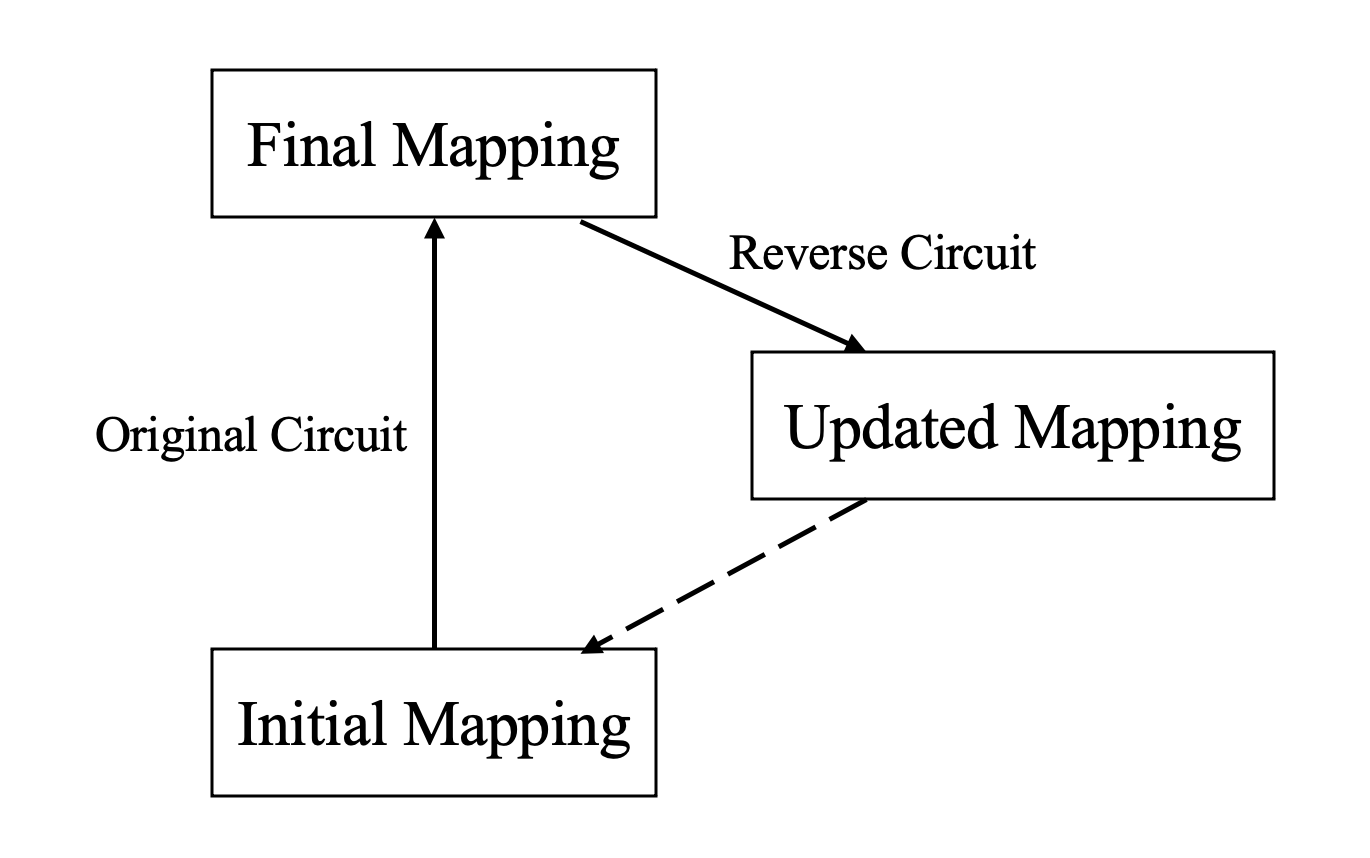
\includegraphics[width=0.45\textwidth]{8.2_figures/initial_mapping.png}
	\caption{初始映射更新过程。}
	\label{fig:qubit-mapping-initial-mapping}
\end{figure}

下面介绍如何在 \MindQuantum\ 中使用 SABRE。可以使用 \code{QubitNode} 和 \code{QubitsTopology} 生成物理拓扑图。

\begin{lstlisting}
from mindquantum.device import QubitNode, QubitsTopology
from mindquantum.io.display import draw_topology

n: int = 5
topology = QubitsTopology([QubitNode(i, poi_x=i) for i in range(n)])
draw_topology(topology)
\end{lstlisting}

上述代码定义了一个包含 5 个节点的拓扑图。\code{QubitNode(i, poi_x=i)} 定义了一个 ID 为 \code{i}、x 轴坐标为 \code{i} 的 \code{QubitNode}。\code{draw_topology} 用于绘制图 \ref{fig:qubit-mapping-topo1} 所示的 SVG。

\begin{figure}
	\centering
	\begin{subfigure}{0.2\textwidth}
		\centering
		
\includegraphics[width=0.8\textwidth]{8.2_figures/topo_1}
		\caption{非连通图。}
		\label{fig:qubit-mapping-topo1}
	\end{subfigure}
	\begin{subfigure}{0.2\textwidth}
		\centering
		
\includegraphics[width=0.8\textwidth]{8.2_figures/topo_2}
		\caption{连通图。}
		\label{fig:qubit-mapping-topo2}
	\end{subfigure}
	\caption{定义一个包含 5 个节点的拓扑图。}
\end{figure}

也可以使用 \code{q1 >> q2} 或 \code{q1 << q2} 连接不同节点，并使用 \code{q1 > q2} 或 \code{q1 < q2} 断开节点连接。下面的代码连接图 \ref{fig:qubit-mapping-topo1}，并生成图 \ref{fig:qubit-mapping-topo2}。

\begin{lstlisting}
for i in range(n-1):
    topology[i] << topology[i+1]
draw_topology(topology)
\end{lstlisting}

\MindQuantum\ 还定义了一些有用的结构。下面的代码定义了图 \ref{fig:qubit-mapping-linear} 所示的线性拓扑，以及图 \ref{fig:qubit-mapping-grid1} 所示的网格拓扑。

\begin{lstlisting}
from mindquantum.device import LinearQubits, GridQubits

t1 = LinearQubits(3)
t2 = GridQubits(3,4)
draw_topology(t1)
draw_topology(t2)
\end{lstlisting}

也可以修改已有图。下面的代码会删除一个节点、孤立一个节点、改变一个节点的颜色、改变一个节点的位置，并添加一条新边。图 \ref{fig:qubit-mapping-grid2} 展示了修改后的图。

\begin{figure}[H]
	\centering

	\begin{subfigure}{0.1\textwidth}
		
\includegraphics[width=0.9\textwidth]{8.2_figures/linear}
		\caption{线性拓扑。}
		\label{fig:qubit-mapping-linear}
	\end{subfigure}
	\begin{subfigure}{0.15\textwidth}
		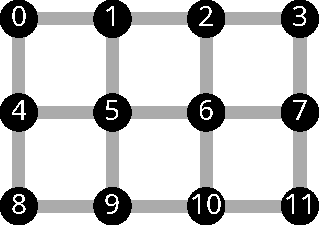
\includegraphics[width=0.9\textwidth]{8.2_figures/grid1}
		\caption{网格拓扑。}
		\label{fig:qubit-mapping-grid1}
	\end{subfigure}
	\begin{subfigure}{0.2\textwidth}
		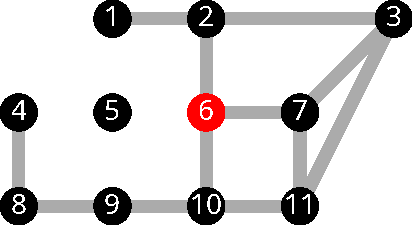
\includegraphics[width=0.9\textwidth]{8.2_figures/grid2}
		\caption{修改后拓扑。}
		\label{fig:qubit-mapping-grid2}
	\end{subfigure}

	\caption{若干常用结构与修改后的拓扑图。}
\end{figure}

\begin{lstlisting}
t2.remove_qubit_node(0)
t2.isolate_with_near(5)
t2.set_color(6, "#ff0000")
t2.set_position(3, 4, 0)
t2[3] << t2[11]
draw_topology(t2)
\end{lstlisting}

结合给定拓扑图，可以使用 SABRE 算法为任意逻辑量子线路生成量子比特映射。下面的代码定义了一个拓扑图 \code{topo} 和一个逻辑线路 \code{circ}。SABRE 求解器需要 4 个参数：
\begin{itemize}
	\item \code{iter_num}：生成初始映射的迭代次数。
	\item \code{w}：式 \eqref{eq:qubit-mapping-h} 中的 $W$ 参数。
	\item \code{delta1}：单量子比特门的衰减参数。
	\item \code{delta2}：CNOT 门的衰减参数。
\end{itemize}
求解器返回三部分：
\begin{itemize}
	\item \code{new_circ}：物理线路。
	\item \code{initial_mapping}：表示初始映射的列表。这里，小写 $q$ 表示逻辑量子比特，大写 $Q$ 表示物理量子比特。例如，\code{[3, 2, 0, 1]} 表示逻辑 $q_0$ 存储在物理 $Q_3$ 上，$q_1$ 存储在 $Q_2$ 上，$q_2$ 存储在 $Q_0$ 上，$q_3$ 存储在 $Q_1$ 上。
	\item \code{final_mapping}：表示最终映射的列表。
\end{itemize}
图 \ref{fig:qubit-mapping-physical-circuit} 展示了一种可能的解。

\begin{lstlisting}
topo = GridQubits(2, 2)
display_svg(draw_topology(topo))

from mindquantum.core.circuit import Circuit
from mindquantum.algorithm.mapping import SABRE

circ = Circuit().h(0).h(1).h(2).x(1, 0).x(2, 1).x(0, 2)
print("Logical circuit:")
display_svg(circ.svg())

solver = SABRE(circ, topo)
new_circ, init_mapping, final_mapping = solver.solve(5, 0.5, 0.3, 0.2)
print("Physical circuit:")
print(f"initial mapping: {init_mapping}")
print(f"  final mapping: {final_mapping}")
display_svg(new_circ.svg())
\end{lstlisting}

\begin{figure}
	\centering
	\begin{subfigure}{0.1\textwidth}
		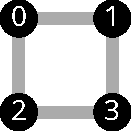
\includegraphics[width=0.8\textwidth]{8.2_figures/topo_3}
		\caption{物理拓扑图。}
		\label{fig:qubit-mapping-physical-topo}
	\end{subfigure}
	\begin{subfigure}{0.35\textwidth}
		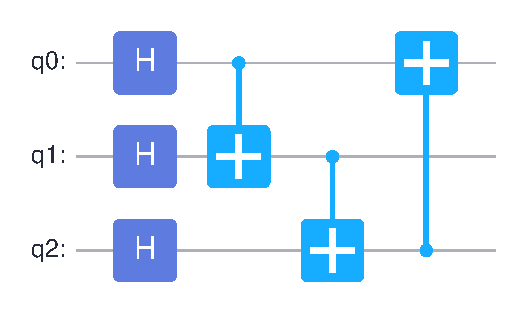
\includegraphics[width=\textwidth]{8.2_figures/logical}
		\caption{逻辑线路。}
		\label{fig:qubit-mapping-logical-circuit}
	\end{subfigure}
	\begin{subfigure}{0.45\textwidth}
		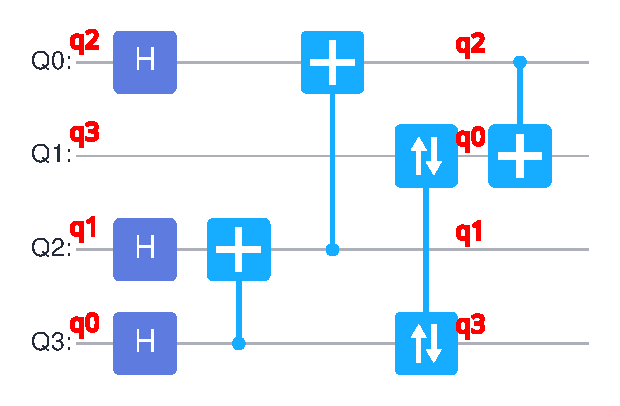
\includegraphics[width=0.9\textwidth]{8.2_figures/physical}
		\caption{一种可能的物理线路。初始映射为 \code{[3, 2, 0, 1]}，最终映射为 \code{[1, 2, 0, 3]}。}
		\label{fig:qubit-mapping-physical-circuit}
	\end{subfigure}

	\caption{SABRE 算法示例。}
\end{figure}

该实现也存在一些不足。目前 \MindQuantum\ 仅支持连通拓扑图。如果物理拓扑不连通，用户必须手动将逻辑量子比特分配到物理连通子图中。
另一个限制是门类型。当前版本只支持单量子比特门和 CNOT 门。由于任意量子线路都可以由单量子比特门和 CNOT 门实现，因此这并不是严重问题。

% Test \code{hello world} .
% - Eq.~\eqref{}
% - Fig.~\ref{}
% - \code{}


% \subsection{Quantum Virtual Machine}
% 设计原理：说明 \MindQuantum\ 如何基于噪声模拟、线路编译和量子比特映射完成量子芯片仿真任务。

使用方法：介绍已定义 QVM 的调用方式，以及如何连接真实量子硬件并执行任务。


% \subsection{Third-party Quantum Chip}
% 概述第三方量子芯片接入方式。

通过示例展示如何配置后端、提交线路任务并获取运行结果。


\section{总结}
\label{sec:summary}
\MindQuantum\ 是一个量子-经典混合框架，聚焦于 NISQ 算法，尤其是变分量子算法的设计与实现。本文首先展示了用于操作量子门、量子线路和可观测量的 eDSL（嵌入式领域专用语言）。\MindQuantum\ 支持在任意量子门上设置任意控制量子比特，并基于 JIT 支持高性能的自定义参数化或非参数化量子门。随后，本文说明了状态矢量、密度矩阵、含噪量子模拟器以及面向量子化学 VQE 的 \texttt{mqchem} CI 子空间模拟器的实现方式，并说明如何通过基于量子门的优化结合 SIMD、OpenMP、鲲鹏和 GPU 加速来优化模拟性能。此外，本文提供了大量应用示例，帮助读者快速掌握 \MindQuantum\ 的用法；这些应用包括 VQE、QAOA 和 QNN。在第~\ref{sec:benchmark} 章中，我们展示了与其他量子框架的性能基准对比，结果表明 \MindQuantum\ 在多个场景下具有优势。最后，本文还展示了我们在真实量子芯片上快速编译并执行量子线路方面所完成的工作。

\section{致谢}
\label{sec:acknowledgement}
我们诚挚感谢本文作者及其各自贡献，具体如表 \ref{tab:contributions} 所示。

\begin{table}[ht]
    \begin{tabular}{|p{3cm}|p{3cm}|}
        \toprule
        作者          & 章节                                           \\
        \midrule
        Qingyu Li     & 2.1, 2.2, 5.3                                  \\
        Qiang Zheng   & 2.3                                            \\
        Jiale Liu     & 2.4                                            \\
        Yanling Lin   & 2.5, 5.9                                       \\
        Xusheng Xu    & 1, 2.6, 3.1, 3.2, 3.3, 4.1, 6.1, 7, 8.1, 9, 10 \\
        Zuoheng Zou   & 6.2, 6.3, 7                                    \\
        Junyuan Zhou  & 3.3, 4.2, 4.3, 7                               \\
        Xu Zhou       & 5.1                                            \\
        Jialiang Tang & 5.2                                            \\
        Ruoqian Xu    & 5.4                                            \\
        Chufan Lyu    & 5.5                                            \\
        Runhong He    & 5.6                                            \\
        Runqiu Shu    & 5.7                                            \\
        Zidong Cui    & 5.8, 6.4                                       \\
        Yikang Zhu    & 8.2                                            \\
        \bottomrule
    \end{tabular}
    \caption{作者贡献}
    \label{tab:contributions}
\end{table}

感谢 Shu Xu、Maolin Luo、Shijie Pan 和 Mosharev Pavel 对本文进行审阅。我们也感谢 Damien Ngyuen、Kai Zhang、Qin Li、Jinlin Zeng、Qi Yan、FangFang Yi、Youkun Ren、Hui Yang、Jiwei Xie、Ting Wang、Haoran Yang、YiXing Feng、Ting Wang、Han Yu、Xiaoling Huan、Jianing Luo 以及许多其他成员在持续集成与文档方面作出的贡献，并感谢 Shenyu Huang、Xiaopeng Cui、Bowen Liu、Yao Wang 在推广方面作出的贡献。我们向 \MindQuantum\ 的所有贡献者和用户致以感谢。正是大家共同的努力与关注，推动着这个项目持续前进。
本工作受到国家自然科学基金项目（批准号：62273154）、中国博士后科学基金项目（批准号：2023M740874）以及国家留学基金委（CSC）项目（批准号：202206890003 和 202306890004）的支持。
\bibliography{lib.bib}

\end{document}
